
%% bare_jrnl.tex
%% V1.3
%% 2007/01/11
%% by Michael Shell
%% see http://www.michaelshell.org/
%% for current contact information.
%%
%% This is a skeleton file demonstrating the use of IEEEtran.cls
%% (requires IEEEtran.cls version 1.7 or later) with an IEEE journal paper.
%%
%% Support sites:
%% http://www.michaelshell.org/tex/ieeetran/
%% http://www.ctan.org/tex-archive/macros/latex/contrib/IEEEtran/
%% and
%% http://www.ieee.org/



% *** Authors should verify (and, if needed, correct) their LaTeX system  ***
% *** with the testflow diagnostic prior to trusting their LaTeX platform ***
% *** with production work. IEEE's font choices can trigger bugs that do  ***
% *** not appear when using other class files.                            ***
% The testflow support page is at:
% http://www.michaelshell.org/tex/testflow/


%%*************************************************************************
%% Legal Notice:
%% This code is offered as-is without any warranty either expressed or
%% implied; without even the implied warranty of MERCHANTABILITY or
%% FITNESS FOR A PARTICULAR PURPOSE! 
%% User assumes all risk.
%% In no event shall IEEE or any contributor to this code be liable for
%% any damages or losses, including, but not limited to, incidental,
%% consequential, or any other damages, resulting from the use or misuse
%% of any information contained here.
%%
%% All comments are the opinions of their respective authors and are not
%% necessarily endorsed by the IEEE.
%%
%% This work is distributed under the LaTeX Project Public License (LPPL)
%% ( http://www.latex-project.org/ ) version 1.3, and may be freely used,
%% distributed and modified. A copy of the LPPL, version 1.3, is included
%% in the base LaTeX documentation of all distributions of LaTeX released
%% 2003/12/01 or later.
%% Retain all contribution notices and credits.
%% ** Modified files should be clearly indicated as such, including  **
%% ** renaming them and changing author support contact information. **
%%
%% File list of work: IEEEtran.cls, IEEEtran_HOWTO.pdf, bare_adv.tex,
%%                    bare_conf.tex, bare_jrnl.tex, bare_jrnl_compsoc.tex
%%*************************************************************************

% Note that the a4paper option is mainly intended so that authors in
% countries using A4 can easily print to A4 and see how their papers will
% look in print - the typesetting of the document will not typically be
% affected with changes in paper size (but the bottom and side margins will).
% Use the testflow package mentioned above to verify correct handling of
% both paper sizes by the user's LaTeX system.
%
% Also note that the "draftcls" or "draftclsnofoot", not "draft", option
% should be used if it is desired that the figures are to be displayed in
% draft mode.
%
\documentclass[journal]{IEEEtran}
\usepackage{blindtext}
\usepackage{graphicx}

% Some very useful LaTeX packages include:
% (uncomment the ones you want to load)


% *** MISC UTILITY PACKAGES ***
%
%\usepackage{ifpdf}
% Heiko Oberdiek's ifpdf.sty is very useful if you need conditional
% compilation based on whether the output is pdf or dvi.
% usage:
% \ifpdf
%   % pdf code
% \else
%   % dvi code
% \fi
% The latest version of ifpdf.sty can be obtained from:
% http://www.ctan.org/tex-archive/macros/latex/contrib/oberdiek/
% Also, note that IEEEtran.cls V1.7 and later provides a builtin
% \ifCLASSINFOpdf conditional that works the same way.
% When switching from latex to pdflatex and vice-versa, the compiler may
% have to be run twice to clear warning/error messages.






% *** CITATION PACKAGES ***
%
%\usepackage{cite}
% cite.sty was written by Donald Arseneau
% V1.6 and later of IEEEtran pre-defines the format of the cite.sty package
% \cite{} output to follow that of IEEE. Loading the cite package will
% result in citation numbers being automatically sorted and properly
% "compressed/ranged". e.g., [1], [9], [2], [7], [5], [6] without using
% cite.sty will become [1], [2], [5]--[7], [9] using cite.sty. cite.sty's
% \cite will automatically add leading space, if needed. Use cite.sty's
% noadjust option (cite.sty V3.8 and later) if you want to turn this off.
% cite.sty is already installed on most LaTeX systems. Be sure and use
% version 4.0 (2003-05-27) and later if using hyperref.sty. cite.sty does
% not currently provide for hyperlinked citations.
% The latest version can be obtained at:
% http://www.ctan.org/tex-archive/macros/latex/contrib/cite/
% The documentation is contained in the cite.sty file itself.






% *** GRAPHICS RELATED PACKAGES ***
%
\ifCLASSINFOpdf
  % \usepackage[pdftex]{graphicx}
  % declare the path(s) where your graphic files are
  % \graphicspath{{../pdf/}{../jpeg/}}
  % and their extensions so you won't have to specify these with
  % every instance of \includegraphics
  % \DeclareGraphicsExtensions{.pdf,.jpeg,.png}
\else
  % or other class option (dvipsone, dvipdf, if not using dvips). graphicx
  % will default to the driver specified in the system graphics.cfg if no
  % driver is specified.
  % \usepackage[dvips]{graphicx}
  % declare the path(s) where your graphic files are
  % \graphicspath{{../eps/}}
  % and their extensions so you won't have to specify these with
  % every instance of \includegraphics
  % \DeclareGraphicsExtensions{.eps}
\fi
% graphicx was written by David Carlisle and Sebastian Rahtz. It is
% required if you want graphics, photos, etc. graphicx.sty is already
% installed on most LaTeX systems. The latest version and documentation can
% be obtained at: 
% http://www.ctan.org/tex-archive/macros/latex/required/graphics/
% Another good source of documentation is "Using Imported Graphics in
% LaTeX2e" by Keith Reckdahl which can be found as epslatex.ps or
% epslatex.pdf at: http://www.ctan.org/tex-archive/info/
%
% latex, and pdflatex in dvi mode, support graphics in encapsulated
% postscript (.eps) format. pdflatex in pdf mode supports graphics
% in .pdf, .jpeg, .png and .mps (metapost) formats. Users should ensure
% that all non-photo figures use a vector format (.eps, .pdf, .mps) and
% not a bitmapped formats (.jpeg, .png). IEEE frowns on bitmapped formats
% which can result in "jaggedy"/blurry rendering of lines and letters as
% well as large increases in file sizes.
%
% You can find documentation about the pdfTeX application at:
% http://www.tug.org/applications/pdftex





% *** MATH PACKAGES ***
%
%\usepackage[cmex10]{amsmath}
% A popular package from the American Mathematical Society that provides
% many useful and powerful commands for dealing with mathematics. If using
% it, be sure to load this package with the cmex10 option to ensure that
% only type 1 fonts will utilized at all point sizes. Without this option,
% it is possible that some math symbols, particularly those within
% footnotes, will be rendered in bitmap form which will result in a
% document that can not be IEEE Xplore compliant!
%
% Also, note that the amsmath package sets \interdisplaylinepenalty to 10000
% thus preventing page breaks from occurring within multiline equations. Use:
%\interdisplaylinepenalty=2500
% after loading amsmath to restore such page breaks as IEEEtran.cls normally
% does. amsmath.sty is already installed on most LaTeX systems. The latest
% version and documentation can be obtained at:
% http://www.ctan.org/tex-archive/macros/latex/required/amslatex/math/





% *** SPECIALIZED LIST PACKAGES ***
%
%\usepackage{algorithmic}
% algorithmic.sty was written by Peter Williams and Rogerio Brito.
% This package provides an algorithmic environment fo describing algorithms.
% You can use the algorithmic environment in-text or within a figure
% environment to provide for a floating algorithm. Do NOT use the algorithm
% floating environment provided by algorithm.sty (by the same authors) or
% algorithm2e.sty (by Christophe Fiorio) as IEEE does not use dedicated
% algorithm float types and packages that provide these will not provide
% correct IEEE style captions. The latest version and documentation of
% algorithmic.sty can be obtained at:
% http://www.ctan.org/tex-archive/macros/latex/contrib/algorithms/
% There is also a support site at:
% http://algorithms.berlios.de/index.html
% Also of interest may be the (relatively newer and more customizable)
% algorithmicx.sty package by Szasz Janos:
% http://www.ctan.org/tex-archive/macros/latex/contrib/algorithmicx/




% *** ALIGNMENT PACKAGES ***
%
%\usepackage{array}
% Frank Mittelbach's and David Carlisle's array.sty patches and improves
% the standard LaTeX2e array and tabular environments to provide better
% appearance and additional user controls. As the default LaTeX2e table
% generation code is lacking to the point of almost being broken with
% respect to the quality of the end results, all users are strongly
% advised to use an enhanced (at the very least that provided by array.sty)
% set of table tools. array.sty is already installed on most systems. The
% latest version and documentation can be obtained at:
% http://www.ctan.org/tex-archive/macros/latex/required/tools/


%\usepackage{mdwmath}
%\usepackage{mdwtab}
% Also highly recommended is Mark Wooding's extremely powerful MDW tools,
% especially mdwmath.sty and mdwtab.sty which are used to format equations
% and tables, respectively. The MDWtools set is already installed on most
% LaTeX systems. The lastest version and documentation is available at:
% http://www.ctan.org/tex-archive/macros/latex/contrib/mdwtools/


% IEEEtran contains the IEEEeqnarray family of commands that can be used to
% generate multiline equations as well as matrices, tables, etc., of high
% quality.


%\usepackage{eqparbox}
% Also of notable interest is Scott Pakin's eqparbox package for creating
% (automatically sized) equal width boxes - aka "natural width parboxes".
% Available at:
% http://www.ctan.org/tex-archive/macros/latex/contrib/eqparbox/





% *** SUBFIGURE PACKAGES ***
%\usepackage[tight,footnotesize]{subfigure}
% subfigure.sty was written by Steven Douglas Cochran. This package makes it
% easy to put subfigures in your figures. e.g., "Figure 1a and 1b". For IEEE
% work, it is a good idea to load it with the tight package option to reduce
% the amount of white space around the subfigures. subfigure.sty is already
% installed on most LaTeX systems. The latest version and documentation can
% be obtained at:
% http://www.ctan.org/tex-archive/obsolete/macros/latex/contrib/subfigure/
% subfigure.sty has been superceeded by subfig.sty.



%\usepackage[caption=false]{caption}
%\usepackage[font=footnotesize]{subfig}
% subfig.sty, also written by Steven Douglas Cochran, is the modern
% replacement for subfigure.sty. However, subfig.sty requires and
% automatically loads Axel Sommerfeldt's caption.sty which will override
% IEEEtran.cls handling of captions and this will result in nonIEEE style
% figure/table captions. To prevent this problem, be sure and preload
% caption.sty with its "caption=false" package option. This is will preserve
% IEEEtran.cls handing of captions. Version 1.3 (2005/06/28) and later 
% (recommended due to many improvements over 1.2) of subfig.sty supports
% the caption=false option directly:
%\usepackage[caption=false,font=footnotesize]{subfig}
%
% The latest version and documentation can be obtained at:
% http://www.ctan.org/tex-archive/macros/latex/contrib/subfig/
% The latest version and documentation of caption.sty can be obtained at:
% http://www.ctan.org/tex-archive/macros/latex/contrib/caption/




% *** FLOAT PACKAGES ***
%
%\usepackage{fixltx2e}
% fixltx2e, the successor to the earlier fix2col.sty, was written by
% Frank Mittelbach and David Carlisle. This package corrects a few problems
% in the LaTeX2e kernel, the most notable of which is that in current
% LaTeX2e releases, the ordering of single and double column floats is not
% guaranteed to be preserved. Thus, an unpatched LaTeX2e can allow a
% single column figure to be placed prior to an earlier double column
% figure. The latest version and documentation can be found at:
% http://www.ctan.org/tex-archive/macros/latex/base/



%\usepackage{stfloats}
% stfloats.sty was written by Sigitas Tolusis. This package gives LaTeX2e
% the ability to do double column floats at the bottom of the page as well
% as the top. (e.g., "\begin{figure*}[!b]" is not normally possible in
% LaTeX2e). It also provides a command:
%\fnbelowfloat
% to enable the placement of footnotes below bottom floats (the standard
% LaTeX2e kernel puts them above bottom floats). This is an invasive package
% which rewrites many portions of the LaTeX2e float routines. It may not work
% with other packages that modify the LaTeX2e float routines. The latest
% version and documentation can be obtained at:

% http://www.ctan.org/tex-archive/macros/latex/contrib/sttools/
% Documentation is contained in the stfloats.sty comments as well as in the
% presfull.pdf file. Do not use the stfloats baselinefloat ability as IEEE
% does not allow \baselineskip to stretch. Authors submitting work to the
% IEEE should note that IEEE rarely uses double column equations and
% that authors should try to avoid such use. Do not be tempted to use the
% cuted.sty or midfloat.sty packages (also by Sigitas Tolusis) as IEEE does
% not format its papers in such ways.


%\ifCLASSOPTIONcaptionsoff
%  \usepackage[nomarkers]{endfloat}
% \let\MYoriglatexcaption\caption
% \renewcommand{\caption}[2][\relax]{\MYoriglatexcaption[#2]{#2}}
%\fi
% endfloat.sty was written by James Darrell McCauley and Jeff Goldberg.
% This package may be useful when used in conjunction with IEEEtran.cls'
% captionsoff option. Some IEEE journals/societies require that submissions
% have lists of figures/tables at the end of the paper and that
% figures/tables without any captions are placed on a page by themselves at
% the end of the document. If needed, the draftcls IEEEtran class option or
% \CLASSINPUTbaselinestretch interface can be used to increase the line
% spacing as well. Be sure and use the nomarkers option of endfloat to
% prevent endfloat from "marking" where the figures would have been placed
% in the text. The two hack lines of code above are a slight modification of
% that suggested by in the endfloat docs (section 8.3.1) to ensure that
% the full captions always appear in the list of figures/tables - even if
% the user used the short optional argument of \caption[]{}.
% IEEE papers do not typically make use of \caption[]'s optional argument,
% so this should not be an issue. A similar trick can be used to disable
% captions of packages such as subfig.sty that lack options to turn off
% the subcaptions:
% For subfig.sty:
% \let\MYorigsubfloat\subfloat
% \renewcommand{\subfloat}[2][\relax]{\MYorigsubfloat[]{#2}}
% For subfigure.sty:
% \let\MYorigsubfigure\subfigure
% \renewcommand{\subfigure}[2][\relax]{\MYorigsubfigure[]{#2}}
% However, the above trick will not work if both optional arguments of
% the \subfloat/subfig command are used. Furthermore, there needs to be a
% description of each subfigure *somewhere* and endfloat does not add
% subfigure captions to its list of figures. Thus, the best approach is to
% avoid the use of subfigure captions (many IEEE journals avoid them anyway)
% and instead reference/explain all the subfigures within the main caption.
% The latest version of endfloat.sty and its documentation can obtained at:
% http://www.ctan.org/tex-archive/macros/latex/contrib/endfloat/
%
% The IEEEtran \ifCLASSOPTIONcaptionsoff conditional can also be used
% later in the document, say, to conditionally put the References on a 
% page by themselves.





% *** PDF, URL AND HYPERLINK PACKAGES ***
%
%\usepackage{url}
% url.sty was written by Donald Arseneau. It provides better support for
% handling and breaking URLs. url.sty is already installed on most LaTeX
% systems. The latest version can be obtained at:
% http://www.ctan.org/tex-archive/macros/latex/contrib/misc/
% Read the url.sty source comments for usage information. Basically,
% \url{my_url_here}.





% *** Do not adjust lengths that control margins, column widths, etc. ***
% *** Do not use packages that alter fonts (such as pslatex).         ***
% There should be no need to do such things with IEEEtran.cls V1.6 and later.
% (Unless specifically asked to do so by the journal or conference you plan
% to submit to, of course. )


% correct bad hyphenation here
\hyphenation{op-tical net-works semi-conduc-tor}


\begin{document}
%
% paper title
% can use linebreaks \\ within to get better formatting as desired
\title{IEEE Journal Template Example}
%
%
% author names and IEEE memberships
% note positions of commas and nonbreaking spaces ( ~ ) LaTeX will not break
% a structure at a ~ so this keeps an author's name from being broken across
% two lines.
% use \thanks{} to gain access to the first footnote area
% a separate \thanks must be used for each paragraph as LaTeX2e's \thanks
% was not built to handle multiple paragraphs
%

\author{Michael~Shell,~\IEEEmembership{Member,~IEEE,}
        John~Doe,~\IEEEmembership{Fellow,~OSA,}
        and~Jane~Doe,~\IEEEmembership{Life~Fellow,~IEEE}% <-this % stops a space
\thanks{M. Shell is with the Department
of Electrical and Computer Engineering, Georgia Institute of Technology, Atlanta,
GA, 30332 USA e-mail: (see http://www.michaelshell.org/contact.html).}% <-this % stops a space
\thanks{J. Doe and J. Doe are with Anonymous University.}% <-this % stops a space
\thanks{Manuscript received April 19, 2005; revised January 11, 2007.}}

% note the % following the last \IEEEmembership and also \thanks - 
% these prevent an unwanted space from occurring between the last author name
% and the end of the author line. i.e., if you had this:
% 
% \author{....lastname \thanks{...} \thanks{...} }
%                     ^------------^------------^----Do not want these spaces!
%
% a space would be appended to the last name and could cause every name on that
% line to be shifted left slightly. This is one of those "LaTeX things". For
% instance, "\textbf{A} \textbf{B}" will typeset as "A B" not "AB". To get
% "AB" then you have to do: "\textbf{A}\textbf{B}"
% \thanks is no different in this regard, so shield the last } of each \thanks
% that ends a line with a % and do not let a space in before the next \thanks.
% Spaces after \IEEEmembership other than the last one are OK (and needed) as
% you are supposed to have spaces between the names. For what it is worth,
% this is a minor point as most people would not even notice if the said evil
% space somehow managed to creep in.



% The paper headers
\markboth{Journal of \LaTeX\ Class Files,~Vol.~6, No.~1, January~2007}%
{Shell \MakeLowercase{\textit{et al.}}: Bare Demo of IEEEtran.cls for Journals}
% The only time the second header will appear is for the odd numbered pages
% after the title page when using the twoside option.
% 
% *** Note that you probably will NOT want to include the author's ***
% *** name in the headers of peer review papers.                   ***
% You can use \ifCLASSOPTIONpeerreview for conditional compilation here if
% you desire.




% If you want to put a publisher's ID mark on the page you can do it like
% this:
%\IEEEpubid{0000--0000/00\$00.00~\copyright~2007 IEEE}
% Remember, if you use this you must call \IEEEpubidadjcol in the second
% column for its text to clear the IEEEpubid mark.



% use for special paper notices
%\IEEEspecialpapernotice{(Invited Paper)}




% make the title area
\maketitle


\begin{abstract}
%\boldmath
\blindtext[1]
\end{abstract}
% IEEEtran.cls defaults to using nonbold math in the Abstract.
% This preserves the distinction between vectors and scalars. However,
% if the journal you are submitting to favors bold math in the abstract,
% then you can use LaTeX's standard command \boldmath at the very start
% of the abstract to achieve this. Many IEEE journals frown on math
% in the abstract anyway.

% Note that keywords are not normally used for peerreview papers.
\begin{IEEEkeywords}
IEEEtran, journal, \LaTeX, paper, template.
\end{IEEEkeywords}






% For peer review papers, you can put extra information on the cover
% page as needed:
% \ifCLASSOPTIONpeerreview
% \begin{center} \bfseries EDICS Category: 3-BBND \end{center}
% \fi
%
% For peerreview papers, this IEEEtran command inserts a page break and
% creates the second title. It will be ignored for other modes.
\IEEEpeerreviewmaketitle



\section{Introduction}
\blindtext

\subsection{Subsection Heading Here}
\blindtext

% needed in second column of first page if using \IEEEpubid
%\IEEEpubidadjcol

% An example of a floating figure using the graphicx package.
% Note that \label must occur AFTER (or within) \caption.
% For figures, \caption should occur after the \includegraphics.
% Note that IEEEtran v1.7 and later has special internal code that
% is designed to preserve the operation of \label within \caption
% even when the captionsoff option is in effect. However, because
% of issues like this, it may be the safest practice to put all your
% \label just after \caption rather than within \caption{}.
%
% Reminder: the "draftcls" or "draftclsnofoot", not "draft", class
% option should be used if it is desired that the figures are to be
% displayed while in draft mode.
%
%\begin{figure}[!t]
%\centering
%\includegraphics[width=2.5in]{myfigure}
% where an .eps filename suffix will be assumed under latex, 
% and a .pdf suffix will be assumed for pdflatex; or what has been declared
% via \DeclareGraphicsExtensions.
%\caption{Simulation Results}
%\label{fig_sim}
%\end{figure}

% Note that IEEE typically puts floats only at the top, even when this
% results in a large percentage of a column being occupied by floats.


% An example of a double column floating figure using two subfigures.
% (The subfig.sty package must be loaded for this to work.)
% The subfigure \label commands are set within each subfloat command, the
% \label for the overall figure must come after \caption.
% \hfil must be used as a separator to get equal spacing.
% The subfigure.sty package works much the same way, except \subfigure is
% used instead of \subfloat.
%
%\begin{figure*}[!t]
%\centerline{\subfloat[Case I]\includegraphics[width=2.5in]{subfigcase1}%
%\label{fig_first_case}}
%\hfil
%\subfloat[Case II]{\includegraphics[width=2.5in]{subfigcase2}%
%\label{fig_second_case}}}
%\caption{Simulation results}
%\label{fig_sim}
%\end{figure*}
%
% Note that often IEEE papers with subfigures do not employ subfigure
% captions (using the optional argument to \subfloat), but instead will
% reference/describe all of them (a), (b), etc., within the main caption.


% An example of a floating table. Note that, for IEEE style tables, the 
% \caption command should come BEFORE the table. Table text will default to
% \footnotesize as IEEE normally uses this smaller font for tables.
% The \label must come after \caption as always.
%
%\begin{table}[!t]
%% increase table row spacing, adjust to taste
%\renewcommand{\arraystretch}{1.3}
% if using array.sty, it might be a good idea to tweak the value of
% \extrarowheight as needed to properly center the text within the cells
%\caption{An Example of a Table}
%\label{table_example}
%\centering
%% Some packages, such as MDW tools, offer better commands for making tables
%% than the plain LaTeX2e tabular which is used here.
%\begin{tabular}{|c||c|}
%\hline
%One & Two\\
%\hline
%Three & Four\\
%\hline
%\end{tabular}
%\end{table}


% Note that IEEE does not put floats in the very first column - or typically
% anywhere on the first page for that matter. Also, in-text middle ("here")
% positioning is not used. Most IEEE journals use top floats exclusively.
% Note that, LaTeX2e, unlike IEEE journals, places footnotes above bottom
% floats. This can be corrected via the \fnbelowfloat command of the
% stfloats package.



\section{Conclusion}
\blindtext





% if have a single appendix:
%\appendix[Proof of the Zonklar Equations]
% or
%\appendix  % for no appendix heading
% do not use \section anymore after \appendix, only \section*
% is possibly needed

% use appendices with more than one appendix
% then use \section to start each appendix
% you must declare a \section before using any
% \subsection or using \label (\appendices by itself
% starts a section numbered zero.)
%


\appendices
\section{Proof of the First Zonklar Equation}
Some text for the appendix.

% use section* for acknowledgement
\section*{Acknowledgment}


The authors would like to thank...


% Can use something like this to put references on a page
% by themselves when using endfloat and the captionsoff option.
\ifCLASSOPTIONcaptionsoff
  \newpage
\fi



% trigger a \newpage just before the given reference
% number - used to balance the columns on the last page
% adjust value as needed - may need to be readjusted if
% the document is modified later
%\IEEEtriggeratref{8}
% The "triggered" command can be changed if desired:
%\IEEEtriggercmd{\enlargethispage{-5in}}

% references section

% can use a bibliography generated by BibTeX as a .bbl file
% BibTeX documentation can be easily obtained at:
% http://www.ctan.org/tex-archive/biblio/bibtex/contrib/doc/
% The IEEEtran BibTeX style support page is at:
% http://www.michaelshell.org/tex/ieeetran/bibtex/
%\bibliographystyle{IEEEtran}
% argument is your BibTeX string definitions and bibliography database(s)
%\bibliography{IEEEabrv,../bib/paper}
%
% <OR> manually copy in the resultant .bbl file
% set second argument of \begin to the number of references
% (used to reserve space for the reference number labels box)
\begin{thebibliography}{1}

\bibitem{IEEEhowto:kopka}
H.~Kopka and P.~W. Daly, \emph{A Guide to \LaTeX}, 3rd~ed.\hskip 1em plus
  0.5em minus 0.4em\relax Harlow, England: Addison-Wesley, 1999.

\end{thebibliography}

% biography section
% 
% If you have an EPS/PDF photo (graphicx package needed) extra braces are
% needed around the contents of the optional argument to biography to prevent
% the LaTeX parser from getting confused when it sees the complicated
% \includegraphics command within an optional argument. (You could create
% your own custom macro containing the \includegraphics command to make things
% simpler here.)
%\begin{biography}[{\includegraphics[width=1in,height=1.25in,clip,keepaspectratio]{mshell}}]{Michael Shell}
% or if you just want to reserve a space for a photo:

\begin{IEEEbiography}[{
\includegraphics[width=1in,height=1.25in,clip,keepaspectratio]{picture}}]{John Doe}
\blindtext
\end{IEEEbiography}

% You can push biographies down or up by placing
% a \vfill before or after them. The appropriate
% use of \vfill depends on what kind of text is
% on the last page and whether or not the columns
% are being equalized.

%\vfill

% Can be used to pull up biographies so that the bottom of the last one
% is flush with the other column.
%\enlargethispage{-5in}

%    Q-circuit version 2
%    Copyright (C) 2004  Steve Flammia & Bryan Eastin
%    Last modified on: 9/16/2011
%
%    This program is free software; you can redistribute it and/or modify
%    it under the terms of the GNU General Public License as published by
%    the Free Software Foundation; either version 2 of the License, or
%    (at your option) any later version.
%
%    This program is distributed in the hope that it will be useful,
%    but WITHOUT ANY WARRANTY; without even the implied warranty of
%    MERCHANTABILITY or FITNESS FOR A PARTICULAR PURPOSE.  See the
%    GNU General Public License for more details.
%
%    You should have received a copy of the GNU General Public License
%    along with this program; if not, write to the Free Software
%    Foundation, Inc., 59 Temple Place, Suite 330, Boston, MA  02111-1307  USA

% Thanks to the Xy-pic guys, Kristoffer H Rose, Ross Moore, and Daniel MÃŒllner,
% for their help in making Qcircuit work with Xy-pic version 3.8.  
% Thanks also to Dave Clader, Andrew Childs, Rafael Possignolo, Tyson Williams,
% Sergio Boixo, Cris Moore, Jonas Anderson, and Stephan Mertens for helping us test 
% and/or develop the new version.

\usepackage{xy}
\xyoption{matrix}
\xyoption{frame}
\xyoption{arrow}
\xyoption{arc}

\usepackage{ifpdf}
\ifpdf
\else
\PackageWarningNoLine{Qcircuit}{Qcircuit is loading in Postscript mode.  The Xy-pic options ps and dvips will be loaded.  If you wish to use other Postscript drivers for Xy-pic, you must modify the code in Qcircuit.tex}
%    The following options load the drivers most commonly required to
%    get proper Postscript output from Xy-pic.  Should these fail to work,
%    try replacing the following two lines with some of the other options
%    given in the Xy-pic reference manual.
\xyoption{ps}
\xyoption{dvips}
\fi

% The following resets Xy-pic matrix alignment to the pre-3.8 default, as
% required by Qcircuit.
\entrymodifiers={!C\entrybox}

\newcommand{\bra}[1]{{\left\langle{#1}\right\vert}}
\newcommand{\ket}[1]{{\left\vert{#1}\right\rangle}}
    % Defines Dirac notation. %7/5/07 added extra braces so that the commands will work in subscripts.
\newcommand{\qw}[1][-1]{\ar @{-} [0,#1]}
    % Defines a wire that connects horizontally.  By default it connects to the object on the left of the current object.
    % WARNING: Wire commands must appear after the gate in any given entry.
\newcommand{\qwx}[1][-1]{\ar @{-} [#1,0]}
    % Defines a wire that connects vertically.  By default it connects to the object above the current object.
    % WARNING: Wire commands must appear after the gate in any given entry.
\newcommand{\cw}[1][-1]{\ar @{=} [0,#1]}
    % Defines a classical wire that connects horizontally.  By default it connects to the object on the left of the current object.
    % WARNING: Wire commands must appear after the gate in any given entry.
\newcommand{\cwx}[1][-1]{\ar @{=} [#1,0]}
    % Defines a classical wire that connects vertically.  By default it connects to the object above the current object.
    % WARNING: Wire commands must appear after the gate in any given entry.
\newcommand{\gate}[1]{*+<.6em>{#1} \POS ="i","i"+UR;"i"+UL **\dir{-};"i"+DL **\dir{-};"i"+DR **\dir{-};"i"+UR **\dir{-},"i" \qw}
    % Boxes the argument, making a gate.
\newcommand{\meter}{*=<1.8em,1.4em>{\xy ="j","j"-<.778em,.322em>;{"j"+<.778em,-.322em> \ellipse ur,_{}},"j"-<0em,.4em>;p+<.5em,.9em> **\dir{-},"j"+<2.2em,2.2em>*{},"j"-<2.2em,2.2em>*{} \endxy} \POS ="i","i"+UR;"i"+UL **\dir{-};"i"+DL **\dir{-};"i"+DR **\dir{-};"i"+UR **\dir{-},"i" \qw}
    % Inserts a measurement meter.
    % In case you're wondering, the constants .778em and .322em specify
    % one quarter of a circle with radius 1.1em.
    % The points added at + and - <2.2em,2.2em> are there to strech the
    % canvas, ensuring that the size is unaffected by erratic spacing issues
    % with the arc.
\newcommand{\measure}[1]{*+[F-:<.9em>]{#1} \qw}
    % Inserts a measurement bubble with user defined text.
\newcommand{\measuretab}[1]{*{\xy*+<.6em>{#1}="e";"e"+UL;"e"+UR **\dir{-};"e"+DR **\dir{-};"e"+DL **\dir{-};"e"+LC-<.5em,0em> **\dir{-};"e"+UL **\dir{-} \endxy} \qw}
    % Inserts a measurement tab with user defined text.
\newcommand{\measureD}[1]{*{\xy*+=<0em,.1em>{#1}="e";"e"+UR+<0em,.25em>;"e"+UL+<-.5em,.25em> **\dir{-};"e"+DL+<-.5em,-.25em> **\dir{-};"e"+DR+<0em,-.25em> **\dir{-};{"e"+UR+<0em,.25em>\ellipse^{}};"e"+C:,+(0,1)*{} \endxy} \qw}
    % Inserts a D-shaped measurement gate with user defined text.
\newcommand{\multimeasure}[2]{*+<1em,.9em>{\hphantom{#2}} \qw \POS[0,0].[#1,0];p !C *{#2},p \drop\frm<.9em>{-}}
    % Draws a multiple qubit measurement bubble starting at the current position and spanning #1 additional gates below.
    % #2 gives the label for the gate.
    % You must use an argument of the same width as #2 in \ghost for the wires to connect properly on the lower lines.
\newcommand{\multimeasureD}[2]{*+<1em,.9em>{\hphantom{#2}} \POS [0,0]="i",[0,0].[#1,0]="e",!C *{#2},"e"+UR-<.8em,0em>;"e"+UL **\dir{-};"e"+DL **\dir{-};"e"+DR+<-.8em,0em> **\dir{-};{"e"+DR+<0em,.8em>\ellipse^{}};"e"+UR+<0em,-.8em> **\dir{-};{"e"+UR-<.8em,0em>\ellipse^{}},"i" \qw}
    % Draws a multiple qubit D-shaped measurement gate starting at the current position and spanning #1 additional gates below.
    % #2 gives the label for the gate.
    % You must use an argument of the same width as #2 in \ghost for the wires to connect properly on the lower lines.
\newcommand{\control}{*!<0em,.025em>-=-<.2em>{\bullet}}
    % Inserts an unconnected control.
\newcommand{\controlo}{*+<.01em>{\xy -<.095em>*\xycircle<.19em>{} \endxy}}
    % Inserts a unconnected control-on-0.
\newcommand{\ctrl}[1]{\control \qwx[#1] \qw}
    % Inserts a control and connects it to the object #1 wires below.
\newcommand{\ctrlo}[1]{\controlo \qwx[#1] \qw}
    % Inserts a control-on-0 and connects it to the object #1 wires below.
\newcommand{\targ}{*+<.02em,.02em>{\xy ="i","i"-<.39em,0em>;"i"+<.39em,0em> **\dir{-}, "i"-<0em,.39em>;"i"+<0em,.39em> **\dir{-},"i"*\xycircle<.4em>{} \endxy} \qw}
    % Inserts a CNOT target.
\newcommand{\qswap}{*=<0em>{\times} \qw}
    % Inserts half a swap gate.
    % Must be connected to the other swap with \qwx.
\newcommand{\multigate}[2]{*+<1em,.9em>{\hphantom{#2}} \POS [0,0]="i",[0,0].[#1,0]="e",!C *{#2},"e"+UR;"e"+UL **\dir{-};"e"+DL **\dir{-};"e"+DR **\dir{-};"e"+UR **\dir{-},"i" \qw}
    % Draws a multiple qubit gate starting at the current position and spanning #1 additional gates below.
    % #2 gives the label for the gate.
    % You must use an argument of the same width as #2 in \ghost for the wires to connect properly on the lower lines.
\newcommand{\ghost}[1]{*+<1em,.9em>{\hphantom{#1}} \qw}
    % Leaves space for \multigate on wires other than the one on which \multigate appears.  Without this command wires will cross your gate.
    % #1 should match the second argument in the corresponding \multigate.
\newcommand{\push}[1]{*{#1}}
    % Inserts #1, overriding the default that causes entries to have zero size.  This command takes the place of a gate.
    % Like a gate, it must precede any wire commands.
    % \push is useful for forcing columns apart.
    % NOTE: It might be useful to know that a gate is about 1.3 times the height of its contents.  I.e. \gate{M} is 1.3em tall.
    % WARNING: \push must appear before any wire commands and may not appear in an entry with a gate or label.
\newcommand{\gategroup}[6]{\POS"#1,#2"."#3,#2"."#1,#4"."#3,#4"!C*+<#5>\frm{#6}}
    % Constructs a box or bracket enclosing the square block spanning rows #1-#3 and columns=#2-#4.
    % The block is given a margin #5/2, so #5 should be a valid length.
    % #6 can take the following arguments -- or . or _\} or ^\} or \{ or \} or _) or ^) or ( or ) where the first two options yield dashed and
    % dotted boxes respectively, and the last eight options yield bottom, top, left, and right braces of the curly or normal variety.  See the Xy-pic reference manual for more options.
    % \gategroup can appear at the end of any gate entry, but it's good form to pick either the last entry or one of the corner gates.
    % BUG: \gategroup uses the four corner gates to determine the size of the bounding box.  Other gates may stick out of that box.  See \prop.

\newcommand{\rstick}[1]{*!L!<-.5em,0em>=<0em>{#1}}
    % Centers the left side of #1 in the cell.  Intended for lining up wire labels.  Note that non-gates have default size zero.
\newcommand{\lstick}[1]{*!R!<.5em,0em>=<0em>{#1}}
    % Centers the right side of #1 in the cell.  Intended for lining up wire labels.  Note that non-gates have default size zero.
\newcommand{\ustick}[1]{*!D!<0em,-.5em>=<0em>{#1}}
    % Centers the bottom of #1 in the cell.  Intended for lining up wire labels.  Note that non-gates have default size zero.
\newcommand{\dstick}[1]{*!U!<0em,.5em>=<0em>{#1}}
    % Centers the top of #1 in the cell.  Intended for lining up wire labels.  Note that non-gates have default size zero.
\newcommand{\Qcircuit}{\xymatrix @*=<0em>}
    % Defines \Qcircuit as an \xymatrix with entries of default size 0em.
\newcommand{\link}[2]{\ar @{-} [#1,#2]}
    % Draws a wire or connecting line to the element #1 rows down and #2 columns forward.
\newcommand{\pureghost}[1]{*+<1em,.9em>{\hphantom{#1}}}
    % Same as \ghost except it omits the wire leading to the left. 

\section{Linear Algebra Section}
LINEAR ALGEBRA SECTION.
The String Matching Problem is generalized into the \textit{exact} string matching and \textit{approximate} string matching variants. In exact string matching, exact copies of a shorter sequence of symbols (pattern) need to be found in a much longer sequence of symbols (text) but the criteria of a match is defined specific to the application of interest \cite{Baker1993,Amir1995}. In approximate string matching a distance metric is defined for measuring nearness of a candidate match, \textit{i.e. Hamming distance, Edit distance}, and all text locations satisfying an mismatch count threshold, \textit{distance}, are returned as solution.

We first define some convention on the notations which we will use in this work. The following is a list of notations we will use throughout this document. 
\begin{itemize}
	\item $\Sigma$ - alphabet; set of symbols in which the pattern and text are defined
	\item $\vert \Sigma \vert$ - the size of $\Sigma$
	\item T - text; a long sequence of symbols from which we will search a shorter sequence of symbols
	\item \textit{N} - the length of T
	\item $\mathrm{T}[i],\ldots,\mathrm{T}[i+M-1]$ - an \textit{M}-length subsequence of T starting at index \textit{i}
	\item P - pattern; a much shorter sequence of symbols which we need to find from the text
	\item \textit{M} - the length of P
	\item $\mathrm{P}_{\Sigma}$ - alphabet of P; the set of all distinct symbols in P
\end{itemize}

In the exact string matching a text T and a pattern P is given as input and the task is to find an exact copy, or copies, of P in T. The output of an algorithm solving the exact string matching problem is the index, or indices, in T in which an exact copy of P occurs. Formally, this problem is defined as follows:\newline
\newline
	\textbf{Exact String Matching Problem} \\
	\begin{tabular}{ l  p{10cm}}
		\textit{Input:} & alphabet $\Sigma$, text $\mathrm{T} \in \Sigma^N$, pattern $\mathrm{P} \in \Sigma^M$\\
		\textit{Output:} & an index \textit{i} where $\mathrm{T}[i],\ldots,\mathrm{T}[i+M-1]=\mathrm{P}$
	\end{tabular}\newline
	
On the other hand, in approximate string matching the task is to find copies of P in T which may have some mismatches up to some defined threshold distance \textit{d}. Variants of this problem may require returning only the first or all solution indices in T. Formally this problem is defined as follows:\newline
\newline	
	\textbf{Approximate String Matching Problem}\\
	\begin{tabular}{ l  p{10cm}}
		\textit{Input:} & alphabet $\Sigma$, text $\mathrm{T} \in \Sigma^N$, pattern $\mathrm{P} \in \Sigma^M$, threshold distance $d < M,N$ defined with respect to some distance metric $Dist(\cdot,\cdot)$\\
		\textit{Output:} & an index \textit{i} where $Dist(\mathrm{T}[i],\ldots,\mathrm{T}[i+M-1],\mathrm{P}) \leq d$
	\end{tabular}\newline

Several distance metrics has been designed to model different problems of applications of the approximate string matching problem. In this thesis, we use a more basic distance metric, called \textit{Hamming distance} for quantifying the distance between any \textit{M}-length subsequence of T and P. Given a subsequence $\mathrm{T}[i],\ldots,\mathrm{T}[i+M-1]$ and P, the Hamming distance between the two sequences in denoted as $H\left( \mathrm{T}[i],\ldots,\mathrm{T}[i+M-1], P \right)$ and is defined as
\[
	H\left( \mathrm{T}[i],\ldots,\mathrm{T}[i+M-1], P \right) = \sum_{j=0}^{M-1} \delta(j)
\] 
where $\delta(\cdot)$ is a function given by
\[
	\delta(j)=
	\begin{cases}
		1, & \text{if}\ \mathrm{P}[j] = \mathrm{T}[i+j]\\
		0, & \text{otherwise}.
	\end{cases}
\]
\section{Quantum Computing Section}
QUANTUM COMPUTING SECTION.
\section{Oracle Chapter}
ORACLE CHAPTER.
\label{chapter:quantum-convolution}\label{chap:quantum-convolution}
In the previous chapter we presented a quantum algorithm for exact string matching based on amplitude amplification used in Grover's quantum search algorithm. In this chapter we present a quantum algorithm for solving the approximate string matching problem using the concept of convolution of sequences. This algorithm makes use of the Fourier transform used in Shor's period finding algorithm. We present an intuition of the algorithm in Section~\ref{sec:qcon-prelims} and its application to the approximate string matching problem in Section~\ref{sec:application-to-approximate-string-matching}. We analyze the algorithms time and space complexity in Section~\ref{sec:time-space-complexity}. In Section~\ref{sec:sub-routines} we discuss in detail the sub-routines of the algorithm. Lastly, in Section~\ref{sec:quantum-algorithm-2} we define the algorithm.

\section{Preliminary concepts}\label{sec:qcon-prelims}
\subsection{Convolution of sequences}
The concept of \textit{convolution} is intuitively a process of applying some given transformation into an input of which the output describes some sense of correlation or similarity between the individual elements of the input and that of the transformation. Convolution has found application in areas such as linear time-invariant systems in which given an impulse function, an input impulse signal is transformed into an output signal that can be expressed as a linear combination of the transformed individual components of the input signal. Also, in image processing, it is used in identifying a location of a template within a much larger 2-dimensional image. In the resulting convolution of the template and the image, the location of the template in the image has the highest correlation value as compared to other locations in the image.

Convolution is defined on two input sequences of numerical values. An input signal and an impulse function can be expressed as a sequence of numerical values along the time domain while a a 2-dimensional image and a template can be expressed as 2-dimensional matrices of numerical values. We define the concept of convolution formally in Definition~\ref{def:convolution}

\begin{definition}[Convolution of sequence of real number]
	\label{def:convolution}
	The \textbf{convolution} of two sequences of real numbers $x=x_0,\ldots,x_{L-1}, y=y_0,\ldots,y_{L-1}$ is defined to be the sequence $z=z_0,\ldots,z_{L-1}$ given by
	\begin{equation}\label{eqn:convolution}
		z_{i} = \sum_{j=0}^{L-1} x_j \cdot y_{i-j}\ \ \text{for}\ i = 0, 1, \ldots, L-1
	\end{equation}
	where the operation between $x_j$ and $y_{i-j}$ is multiplication and the subscripts are taken (\textrm{mod} L).
\end{definition}
In this work, we use the usual notation $x \ast y$ for the convolution of any two arbitrary sequences $x, y$.

\subsection{Convolution as string matching}
The process of computing for the convolution of two sequences can be interpreted as the process of sliding a short sequence over a much longer sequence one position at a time. The \textit{i}-th value of the convolution of two sequences $x, y$ is given by
\begin{align*}
	z_{i} &= \sum_{j=0}^{L-1} x_j \cdot y_{i-j}\\
	        &= x_{0}\cdot y_{i} + x_{1}\cdot y_{i-1} + x_{2}\cdot y_{i-2} + \ldots + x_{L-1}\cdot y_{i-(L-1)}
\end{align*}
Let
\begin{itemize}
    \item $L=N+M-1$
    \item $x, y \in \{0,1\}^L$
    \item $x[N],\ldots,x[L-1]=0^{M-1}$
    \item $y[M],\ldots,y[L-1]=0^{N-1}$
\end{itemize}
Equation~\ref{eqn:convolution} then corresponds to the number of matching $1$s between the subsequences $x[i],\ldots,x[i+M-1]$ and $y[M-1],\ldots,y[0]$.

Let
\begin{itemize}
    \item $x_{\sigma_k}$ be given by
    	\begin{equation*}
			x[i]_{\sigma_k} =
			\begin{cases}
				1, & \mathrm{if}\ 0 \leq i < N\ \text{and T}[i]=\sigma_k\\
				0, & \mathrm{otherwise} 
			\end{cases}
		\end{equation*}
		for all $i=0,\ldots,L-1$
	\item $y_{\sigma_k}$ be given by
    	\begin{equation*}
			y[i]_{\sigma_k} =
			\begin{cases}
				1, & \mathrm{if}\ 0 \leq i < M\ \text{and P}[M-1-i]=\sigma_k\\
				0, & \mathrm{otherwise} 
			\end{cases}
		\end{equation*}
		for all $i=0,\ldots,L-1$
	\item $z_{\sigma_k} = x_{\sigma_k}*y_{\sigma_k}$
\end{itemize}
$z[i]_{\sigma_k}$ then corresponds to the number of matching presence of symbols $\sigma_k$ between subsequence $\mathrm{T}[i],\ldots,\mathrm{T}[i+M-1]$ and P.

Let
\begin{itemize}
    \item $\mathrm{T} \in \Sigma^{N}, \mathrm{P} \in \Sigma^{M}$ where $\Sigma=\{\sigma_1, \ldots, \sigma_k, \ldots\}$
    \item $x_{\sigma_k}=\mathrm{T}_{\sigma_k}0^{M-1}$ be the binary encoding of T with respect to symbol $\sigma_k$
    \item $y_{\sigma_k}=\mathrm{P}_{\sigma_k}[M-1],\ldots,\mathrm{P}_{\sigma_k}[0],0^{N-1}$ be the binary encoding of the reverse of P with respect to symbol $\sigma_k$
\end{itemize}
The point-wise addition of the convolutions $z_{\sigma_1}, \ldots, z_{\sigma_k}, \ldots$ then corresponds to a sequence $z_{\Sigma}$ given by
\begin{align}
	    z_{\Sigma}[i] &= \sum_{k=1}^{\vert \Sigma \vert} z_{\sigma_k}[i]\\
	                                          &= H\left( \mathrm{P}, \mathrm{T}[i],\ldots,\mathrm{T}[i+M-1] \right)\nonumber
\end{align}
for all $i=0,\ldots,L-1$. $z_{\Sigma}$ is a sequence of Hamming distance between P and each \textit{M}-length subsequence of T. Note that we are only interested with $z[M-1],\ldots,z[N-M+1]$ since 
\[
	z[M-1]=H\left(\mathrm{P}, \mathrm{T}[0],\ldots,\mathrm{T}[M-1]\right)
\]
and 
\[
	z[N-M+1]=H\left( \mathrm{P},\mathrm{T}[N-M+1],\ldots,\mathrm{T}[N-1]\right).
\]
The correspondence between the convolution of two sequences and the sequence of Hamming distance between subsequences of T and P implies that an efficient algorithm for computing the convolution is also an efficient algorithm for string matching. In the succeeding sections we present a quantum algorithm for computing the convolution of two sequences. This quantum algorithm, in specific cases, can be more efficient than its classical counterpart and other quantum algorithms for string matching presented in the previous chapter.

\subsection{Discrete Fourier transform and Convolution theorem}
%In signal processing and analysis, a theorem which describes the relationship between the convolution in the time domain and the frequency domain is the \textit{Convolution theorem}. In this work we use the convolution theorem specific to discrete periodic signals since the binary indicator sequences for the input text and pattern can be viewed as sampling of periodic signals but with noise. The transformation of an arbitrary signal from the time domain to the frequency domain is carried out using \textit{Fourier transform}. Since we are dealing only with discrete information, we are only interested in the \textit{discrete} version of the Fourier transform. 

One area of application of the concept of convolution is digital signal processing. There is a theorem which relates the convolution of two discrete signals in the time domain to operations on some transform of the discrete signals in the frequency domain. Such theorem is the \textit{Convolution theorem} in Theorem~\ref{thm:convolution-theorem}. The transform on the signals is the \textit{Fourier transform} and its inverse.

\begin{definition}[Discrete Fourier transform]
	Given a discrete signal $x=x_0,\ldots,x_{L-1}$, its discrete Fourier transform $X$ is given by
	\[
		X[k] = \frac{1}{\sqrt{L}} \sum_{l=0}^{L-1} x[j] e^{2\pi i k \frac{l}{L}}\ \text{for}\ k=0,\ldots,L-1
	\]
\end{definition}
\begin{definition}[Inverse discrete Fourier transform]
	Given a discrete signal $X$, for $l=0,\ldots,L-1$, its inverse discrete Fourier transform $x$ is given by
	\[
		x[k] = \frac{1}{\sqrt{L}} \sum_{l=0}^{L-1} X[j] e^{-2\pi i k \frac{l}{L}}\ \text{for}\ k=0,\ldots,L-1
	\]
\end{definition}
In this work we denote the discrete Fourier transform as \textit{F} and its inverse as $F^{-1}$.

\begin{theorem}[Convolution theorem]\label{thm:convolution-theorem}
	Given two discrete periodic signals $x=x_0,\ldots,x_{L-1}, y=y_0,\ldots,y_{L-1}$,
	\[
		F\left( x \ast y \right) = F\left( x \right) \cdot F\left( y \right)
	\]
where $\cdot$ denotes point-wise multiplication.
\end{theorem}

According to the Convolution theorem, the convolution in the time domain corresponds to point-wise multiplication in the frequency domain. The interest in the association of the concept of convolution with Fourier transform lies in the the availability of fast computation of the convolution of any two discrete periodic signals through efficient computation of the discrete Fourier transform. One algorithm which does efficient computation of the discrete Fourier transform is the \textit{fast Fourier transform algorithm}. Given an \textit{L}-length discrete signal $x$, its discrete Fourier transform will require $O(L^2)$ operations. The same computation can be achieved with $O(L\log_2(L))$ operations using the fast Fourier transform algorithm.

In this work, we compute for the discrete Fourier transform of a sequence using a quantum computer in the Convolution theorem. The following sections describe details of the quantum Fourier transform and the quantum version of the Convolution theorem. 

\subsection{Quantum Fourier transform}\label{subsec:qft}
The discrete Fourier transform of a sequence can be computed using a quantum computer. In Shor's quantum algorithm for prime factorization\cite{Shor1994}, he demonstrated a polynomial-time construction on a quantum computer for a unitary matrix which corresponds to the discrete Fourier transform. His construction on a quantum computer is for the special case when $L=2^n$, which was independently discovered and analyzed by Coppersmith in \cite{Coppersmith1994} and Barenco et. al in \cite{Barenco1996}. The quantum version of the discrete Fourier transform and its inverse is defined in Definition~\ref{def:qft} and Definition~\ref{def:iqft}.

\begin{definition}[Quantum Fourier transform]\label{def:qft}
	Let $B=\{\vert 0 \rangle, \ldots, \vert L-1 \rangle\}$ be an orthonormal basis for a $L$-dimension complex vector state space. The quantum Fourier transform is defined such that
	\[
		F_{\mathrm{Q}}\left(\vert k \rangle\right) = \frac{1}{\sqrt{L}} \sum_{j=0}^{L-1} e^{2\pi i k \frac{j}{L}} \vert j \rangle \ \ \ \text{ for all } \vert k \rangle \in B
	\]
\end{definition}

\begin{definition}[Inverse quantum Fourier transform]\label{def:iqft}
	Let $B=\{\vert 0 \rangle, \ldots, \vert L-1 \rangle\}$ be an orthonormal basis for a $L$-dimensional complex vector state space. The inverse quantum Fourier transform is defined such that
	\[
		F_{\mathrm{Q}}^{-1}\left(\vert k \rangle\right) = \frac{1}{\sqrt{L}} \sum_{j=0}^{L-1} e^{-2\pi i k \frac{j}{L}} \vert j \rangle \ \ \ \text{ for all } \vert k \rangle \in B
	\]
\end{definition}
The quantum Fourier transform can be implemented as the $L \times L$ unitary matrix given by
\[
	F_{\mathrm{Q}}(k,l) = \frac{1}{\sqrt{L}} e^{2\pi i k\frac{l}{L}}
\]
for all $k,l=0,\ldots,L-1$. Note that this is the same matrix as that of the discrete Fourier Transform. The inverse quantum Fourier transform on the other hand is given by 
\[
	F_{\mathrm{Q}}(k,l) = \frac{1}{\sqrt{L}} e^{-2\pi i k\frac{l}{L}}
\]
for all $k,l=0,\ldots,L-1$. On the other hand, the input sequence can be represented as a $1 \times L$ column vector $\left[ x_0, x_1, \ldots, x_{L-1} \right]^T$. The computation of the fast Fourier transform algorithm requires $O\left(L\log_2(L)\right)$ time complexity. The quantum Fourier transform though, as shown by Shor's quantum network construction, can be implemented using quantum circuit with depth of $O\left( \log_2(L)^2 + \log_2(L) \right)$, which is quadratic in the length of the input $\log_2(L)$. An approximation of the quantum Fourier transform has been shown to reduce the circuit complexity by a constant factor \cite{Coppersmith1994} by discarding some phase factors in the elements of the matrix. 

Since the matrix construction of the quantum Fourier transform is just same with that of the discrete Fourier transform, it seems that we can directly replace the discrete Fourier transform with the quantum Fourier transform in the Convolution theorem. This is not the case though as shown in \cite{Lomont2003}. There is no unitary operation which corresponds to point-wise multiplication of two Fourier transforms. A suggested unitary approximation of the point-wise multiplication in \cite{Curtis2004} is to construct an $L \times L$ matrix $V_{\mathrm{X}}$ of which entries $V_{\mathrm{X}}(i,i)$ correspond to the \textit{normalized entries} of the Fourier transform $\vert X \rangle$ of the input superposition quantum states $\vert x \rangle$ corresponding to input sequence $x[l]$. Note that $V_{\mathrm{X}}(i,i)$ is undefined when $\langle i \myket{X} = 0$. If such is the case, in this study we let $\langle i \myket{X} = \epsilon$ where $\epsilon$ is a very small real number. This implies $V_{\mathrm{X}}(i,i) = 1$ when $\langle i \myket{X} = 0$. We define formally this matrix in Definition~\ref{def:operator-V}.

\begin{definition}[Operator $V_\mathrm{X}$]\label{def:operator-V}
	Given the quantum Fourier transform of an L-dimension quantum state $\vert x \rangle$ spanned by basis set $B=\{\vert 0 \rangle,\ldots,\vert L-1 \rangle\}$,
	\[
		\vert X \rangle = \frac{1}{L} \sum_{j=0}^{L-1} \sum_{k=0}^{L-1} e^{2\pi i k \frac{j}{L} } \vert j \rangle,
	\]
	operator $V_{\mathrm{X}}$ is an $L \times L$ matrix given by
	\[
		V_{\mathrm{X}}(i,j) = 
		\begin{cases}
			\frac{\langle i \vert X \rangle}{\| \langle i \vert X \rangle \|}, & \mathrm{if\ } i=j,\mathrm{\ and\ } \langle i \myket{X} \neq 0,\\
			1,                                                                                       & \mathrm{if\ } i=j,\mathrm{\ and\ } \langle i \myket{X} = 0,\\
			0,                                                                                       & \mathrm{otherwise} 
		\end{cases}
	\]
	for all $i,j = 0,\ldots,L-1$.
\end{definition}

\begin{lemma}
	The operator $V_{\mathrm{X}}$ is a unitary. 
\end{lemma}
\begin{proof}
Since $V_{\mathrm{X}}$ is a diagonal matrix, $V_{\mathrm{X}}V_{\mathrm{X}}^\dagger $ is given by
\begin{equation*}
	\begin{split}
		\frac{\langle i \vert X \rangle}{\| \langle i \vert X \rangle \|}\frac{\langle i \vert X \rangle^\ast}{\| \langle i \vert X \rangle^\ast \|} &= \frac{\langle i \vert X \rangle}{ \sqrt{ \vert \langle i \vert X \rangle \vert^2} }\frac{\langle i \vert X \rangle^\ast}{ \sqrt{ \vert \langle i \vert X \rangle^\ast \vert^2 }}\\
		&= \frac{\langle i \vert X \rangle}{ \sqrt{ \langle i \vert X \rangle\langle i \vert X \rangle^\ast } }\frac{\langle i \vert X \rangle^\ast}{ \sqrt{ \langle i \vert X \rangle^\ast\langle i \vert X \rangle }}\\
		&= \frac{\langle i \vert X \rangle\langle i \vert X \rangle^\ast}{ \left(\sqrt{ \langle i \vert X \rangle\langle i \vert X \rangle^\ast } \right)^2 }\\
		&= \frac{\langle i \vert X \rangle}{ \langle i \vert X \rangle }\frac{\langle i \vert X \rangle^\ast}{ \langle i \vert X \rangle^\ast }\\
		&= 1
	\end{split}
\end{equation*}
for all $i=0,\ldots,L-1$. Thus, $V_{\mathrm{X}}V_{\mathrm{X}}^{\dagger}=I$. It is also easy to see to that $V_{\mathrm{X}}^{\dagger}V_{\mathrm{X}}=I$.
\end{proof}
Using the same analysis we used for the amplitude amplification operator $W$ in the previous chapter, we analyze the circuit and time complexity of operator $V_{\mathrm{X}}$. Since the elements along the diagonal of $V_{\mathrm{X}}$ will be less likely regular as composed to those along the diagonal of $W$, the phase context decomposition of operator $V_{\mathrm{X}}$ will require more than one single-parameter operators $V\left( \phi_i, l_i \right)$. Let \textit{q} be the number of distinct phase values $\phi_i$ along the diagonal of $V_{\mathrm{X}}$. The circuit complexity of approximating $V_{\mathrm{X}}$ using the Clifford+\textit{T} gate set will then be 
\[
	(q-1)C_0\log_2 \left( \frac{1}{\epsilon} \right) + \Om\left( \log\log \left(\frac{1}{\epsilon}\right) + (q-1)\log_2 L \right)
\]
\cite{Bocharov2015}. Assuming a low count of distinct phase values \textit{q} compared to \textit{L}, the circuit complexity of $V_{\mathrm{X}}$ will be in 
\[
	\Om\left( q\log_2 L \right).
\]
We assume the same for its time complexity. $V_{\mathrm{X}}$ will work on the same binary indicator sequence registers from the previous steps and so will work on $\log_2 L$ qubits.

Given the definition of operator $V_{\mathrm{X}}$, we define an approximate quantum version of the convolution theorem in Theorem~\ref{thm:quantum-convolution-theorem}.

\begin{theorem}[Quantum convolution theorem]\label{thm:quantum-convolution-theorem}
	Let $x$ and $y$ be two sequences of length L and $z = x \ast y$. Let $\vert x \rangle, \vert y \rangle, \vert z \rangle$ be quantum state representations of $x, y$ and $z$ spanned by basis set $B=\{\vert 0 \rangle,\ldots,\vert L-1 \rangle\}$, respectively. Given the quantum Fourier transform $\vert Y \rangle$ of $\vert y \rangle$ and the unitary operator $V_{\mathrm{X}}$ constructed from the quantum Fourier transform $\vert X \rangle$ of $\vert x \rangle$,
	\[
		F_{\mathrm{Q}}\left( \vert z \rangle \right) \approx V_{\mathrm{X}} \left(\vert Y \rangle\right)
	\]
where $V_{\mathrm{X}} \left(\vert Y \rangle\right)$ is given by
	\begin{equation*}
		\begin{split}
			\langle i \vert \left(V_{\mathrm{X}} \left(\vert Y \rangle\right)\right) &= \frac{\langle i \vert X \rangle}{\| \langle i \vert X \rangle \|} \langle i \vert Y \rangle
		\end{split}
	\end{equation*}
for all $i=0,\ldots,L-1$.
\end{theorem}
From Theorem~\ref{thm:quantum-convolution-theorem} we can derive an \textit{approximation} of $\vert z \rangle$ by taking the inverse quantum Fourier transform of $V_{\mathrm{X}} \left(\vert Y \rangle\right)$, 
\[
	\vert z \rangle \approx F_{\mathrm{Q}}^{-1}\left( V_{\mathrm{X}}\left( \vert Y \rangle \right) \right).
\]
Since an approximation of \textit{z} is encoded in the quantum state, $F_{\mathrm{Q}}^{-1}\left( V_{\mathrm{X}}\left( \vert Y \rangle \right) \right)$, we can only get one classical output for each measurement of the state of the quantum register. We iterate the quantum convolution algorithm multiple times to obtain multiple classical values corresponding to indices in T. These indices will be interpreted as possible solution starting indices of exact or approximate copies of P in T. Just like in classical convolution, we will only consider the middle $N-M+1$ indices of the convolution as valid candidate solutions. Basic classical verification of an output will only require time complexity linear to the size of the input pattern $M$.

\section{In application to approximate string matching}\label{sec:application-to-approximate-string-matching}
%In \cite{Fischer1974} the concept of convolution was shown to be also applicable to the string matching problem. Given input text T and pattern P, we encode the sequences
%\begin{equation*}
%	\begin{split}
%		\text{T}_{\mathrm{pad}} &= \text{T}[0], \text{T}[1], \ldots, \text{T}[N-1], \ast^{M-1}\\
%		\text{P}_{\mathrm{pad}} &= \text{P}[M-1], \text{P}[M-2], \ldots, \text{P}[0], \ast^{N-1}.
%	\end{split}
%\end{equation*}
%Since we have sequences of symbols to compare, we replace the multiplication operation in the definition of convolution of two sequences of real numbers with a comparison operation. Let $L=N+M-1$. We define the convolution of two sequences of symbols in Definition~\ref{def:convolution-symbols}.
%
%\begin{definition}[Convolution of sequences of symbols]
%	\label{def:convolution-symbols}
%	The \textbf{convolution} of two sequences of symbols $x=\left(x_0,\ldots,x_{L-1}\right)$ and $y=\left(y_0,\ldots,y_{L-1}\right)$ defined over $\Sigma=\{\sigma_0,\ldots,\sigma_{\vert \Sigma \vert-1}\}$ is defined to be the sequence $z=\left(z_0,\ldots,z_{L-1}\right)$ given by
%	\[
%		z_{i} = \sum_{j=0}^{L-1} C(x_j, y_{i-j})\ \ \text{for}\ i = 0, 1, \ldots, L-1
%	\]
%	where C 
%	\[
%		C(x_j, y_{i-j}) =
%		\begin{cases}
%			0,\ \ \mathrm{if}\ x_j \neq y_{i-j}\ \mathrm{OR}\ (x_j = \ast\ \mathrm{OR}\ y_{i-j} = \ast), \\
%			1,\ \ \mathrm{otherwise}.
%		\end{cases}
%	\]
%	and the subscripts are taken (\text{mod} L).
%\end{definition}
%In Definition~\ref{def:convolution-symbols}, we let $x=\text{T}_{\mathrm{pad}}, y=\text{P}_{\mathrm{pad}}$ and \textit{z} the convolution of $\text{T}_{\mathrm{pad}}$ and $\text{P}_{\mathrm{pad}}$. The convolution of $\text{T}_{\mathrm{pad}}$ and $\text{P}_{\mathrm{pad}}$ will be the sequence of match scores for each \textit{M}-length substring of T compared with P, excluding the first and last $M-1$ indices in the convolution. The convolution of $\text{T}_{\mathrm{pad}}$ and $\text{P}_{\mathrm{pad}}$ then provides a solution to the approximate string matching problem if we select the indices \textit{i} in the z such that $M-z_i \leq d$ where \textit{d} is the input distance threshold.
%
%\begin{example}
%	Given input text \textrm{T} = a,a,b,a and pattern \textrm{P} = b,a, we identify the convolution of the sequences 
%		\begin{equation*}
%			\begin{split}
%				\textrm{T}_{\mathrm{pad}} = a,a,b,a,\ast\\
%				\text{P}_{\mathrm{pad}} = a,b,\ast,\ast,\ast
%			\end{split}
%		\end{equation*}
%	where $L = 5$. The convolution of $\text{T}_{\mathrm{pad}}$ and $\text{P}_{\mathrm{pad}}$ is given by
%		\begin{equation*}
%			\begin{split}
%				\gamma_0 &= \sum_{j=0}^{4} C(\text{T}_{\mathrm{pad}}[j],\overleftarrow{\text{P}}_{\mathrm{pad}}[0-j])\\
%				&= C(\text{T}_{\mathrm{pad}}[0],\overleftarrow{\text{P}}_{\mathrm{pad}}[0-0]) + C(\text{T}_{\mathrm{pad}}[1],\overleftarrow{\text{P}}_{\mathrm{pad}}[0-1]) + C(\text{T}_{\mathrm{pad}}[2],\overleftarrow{\text{P}}_{\mathrm{pad}}[0-2])\\
%				&\quad\quad\quad + C(\text{T}_{\mathrm{pad}}[3],\overleftarrow{\text{P}}_{\mathrm{pad}}[0-3]) + C(\text{T}_{\mathrm{pad}}[4],\overleftarrow{\text{P}}_{\mathrm{pad}}[0-4])\\
%				&= C(\text{T}_{\mathrm{pad}}[0],\overleftarrow{\text{P}}_{\mathrm{pad}}[0]) + C(\text{T}_{\mathrm{pad}}[1],\overleftarrow{\text{P}}_{\mathrm{pad}}[4]) + C(\text{T}_{\mathrm{pad}}[2],\overleftarrow{\text{P}}_{\mathrm{pad}}[3])\\
%				&\quad\quad\quad + C(\text{T}_{\mathrm{pad}}[3],\overleftarrow{\text{P}}_{\mathrm{pad}}[2]) + C(\text{T}_{\mathrm{pad}}[4],\overleftarrow{\text{P}}_{\mathrm{pad}}[1])\\
%				&= C(\text{T}_{\mathrm{pad}}[0],\text{P}[1]) + C(\text{T}_{\mathrm{pad}}[1],\ast) + C(\text{T}_{\mathrm{pad}}[2],\ast) + C(\text{T}_{\mathrm{pad}}[3],\ast) + C(\text{T}_{\mathrm{pad}}[4],\text{P}[0])\\
%				&= C\left(a,a \right) + C\left(a,\ast \right) + C\left(b,\ast \right) + C\left(a,\ast \right) + C\left(\ast,b \right)\\
%				&=1 + 0 + 0 + 0 + 0\\
%				&=1
%			\end{split}
%		\end{equation*}
%Following the same computation for $\gamma_1$ to $\gamma_4$, we will have the values $\gamma_1=1, \gamma_2=0, \gamma_3=2, \gamma_4=0$. The convolution of $\text{T}_{\mathrm{pad}}$ and $\overleftarrow{\text{P}}_{\mathrm{pad}}$ is then the sequence 1,1,0,2,0. Excluding the first and last 1 index of the convolution, the index with highest score in the convolution is index 3 which corresponds to index 2 of T. Index 2 of the convolution has score of 2 which corresponds to the number of matches when substring T[2,3] is compared to P.
%\end{example}
%
%\subsection{Binary indicator sequence encoding}
%Since we store data using binary quantum registers, we perform the comparison operation in Definition~\ref{def:convolution-symbols} as a binary operation on binary encoding of T and P. We use a \textit{binary indicator sequence} to encode an input sequence of symbols according to the presence or absence of a specific symbol in the sequence. A bit 1 will indicate the presence of a symbol and a bit 0 for , i.e. including the zero paddings to the right. Given an alphabet $\Sigma=\{\sigma_0,\ldots,\sigma_{\vert \Sigma \vert}\}$ on which the input text and pattern are defined, a binary indicator sequence will be created for each symbol $\sigma_i \in \Sigma$ for each of the text and pattern. We replace the compare operation $C(\cdot,\cdot)$ with the logical operation AND ($\wedge$). We redefine the convolution of two sequences of symbols in Definition~\ref{def:convolution-binary}.
%
%\begin{definition}[Convolution of binary sequences]
%	\label{def:convolution-binary}
%	The \textbf{convolution} of two binary sequences $S_1=\left(\alpha_0,\ldots,\alpha_{N-1}\right)$ and $S_2=\left(\beta_0,\ldots,\beta_{N-1}\right)$ is defined to be the sequence $S_3=\left(\gamma_0,\ldots,\gamma_{N-1}\right)$ given by
%	\[
%		\gamma_{i} = \sum_{j=0}^{N-1} \alpha_j \wedge \beta_{i-j}\ \ \text{for}\ i = 0, 1, \ldots, N-1
%	\]
%	where $\wedge$ is the logical AND operation and the subscripts are taken \text{(mod N)}.
%\end{definition}
%
%\begin{example}
%	Given $\Sigma=\{a,b\}$ and input text \text{T} = a,a,b,a and pattern \text{P} = b,a, we identify the convolution of the pairs of sequences for symbol \textit{a} as
%		\begin{equation*}
%			\begin{split}
%				\text{T}(a)_{\mathrm{pad}} = 1,1,0,1,0\\
%				\overleftarrow{\text{P}}(a)_{\mathrm{pad}} = 1,0,0,0,0
%			\end{split}
%		\end{equation*}
%	and symbol \textit{b} as
%		\begin{equation*}
%			\begin{split}
%				\text{T}(b)_{\mathrm{pad}} = 0,0,1,0,0\\
%				\overleftarrow{\text{P}}(b)_{\mathrm{pad}} = 0,1,0,0,0
%			\end{split}
%		\end{equation*}
%	We compute for the convolution of each pair of binary indicator sequences. The convolution of binary indicator sequences $\text{T}(a)_{\mathrm{pad}}$ and $\overleftarrow{\text{P}}(a)_{\mathrm{pad}}$ is given by
%	\begin{equation*}
%		\begin{split}
%			\gamma_{a_0} &= \sum_{j=0}^{4} \text{T}(a)_{\mathrm{pad}}[j] \wedge \overleftarrow{\text{P}}(b)_{\mathrm{pad}}[0-j]\\
%			&= \text{T}(a)_{\mathrm{pad}}[0] \wedge \overleftarrow{\text{P}}(b)_{\mathrm{pad}}[0-0] + \text{T}(a)_{\mathrm{pad}}[1] \wedge \overleftarrow{\text{P}}(b)_{\mathrm{pad}}[0-1] + \text{T}(a)_{\mathrm{pad}}[2] \wedge \overleftarrow{\text{P}}(b)_{\mathrm{pad}}[0-2]\\
%			&\quad\quad\quad\quad + \text{T}(a)_{\mathrm{pad}}[3] \wedge \overleftarrow{\text{P}}(b)_{\mathrm{pad}}[0-3] + \text{T}(a)_{\mathrm{pad}}[4] \wedge \overleftarrow{\text{P}}(b)_{\mathrm{pad}}[0-4]\\
%			&= \text{T}(a)_{\mathrm{pad}}[0] \wedge \overleftarrow{\text{P}}(b)_{\mathrm{pad}}[0] + \text{T}(a)_{\mathrm{pad}}[1] \wedge \overleftarrow{\text{P}}(b)_{\mathrm{pad}}[4] + \text{T}(a)_{\mathrm{pad}}[2] \wedge \overleftarrow{\text{P}}(b)_{\mathrm{pad}}[3]\\
%			&\quad\quad\quad\quad + \text{T}(a)_{\mathrm{pad}}[3] \wedge \overleftarrow{\text{P}}(b)_{\mathrm{pad}}[2] + \text{T}(a)_{\mathrm{pad}}[4] \wedge \overleftarrow{\text{P}}(b)_{\mathrm{pad}}[1]\\
%			&= 1 \wedge 1 + 1 \wedge 0 + 0 \wedge 0 + 1 \wedge 0 + 0 \wedge 0\\
%			&= 1 + 0 + 0 + 0 + 0\\
%			&= 1
%		\end{split}		
%	\end{equation*}
%	Following the same computation for the other scores, we get the values $\gamma_{a_1}=1, \gamma_{a_2}=0, \gamma_{a_3}=1, \gamma_{a_1}=0$. The convolution of the binary indicator sequences $\text{T}(a)_{\mathrm{pad}}$ and $\overleftarrow{\text{P}}(a)_{\mathrm{pad}}$ is then the sequence  1,1,0,1,0. Computing for the convolution of the binary indicator sequences $\text{T}(b)_{\mathrm{pad}}$ and $\overleftarrow{\text{P}}(b)_{\mathrm{pad}}$ on the other hand will arrive at the sequence 0,0,0,1,0. Adding the corresponding values of the two convolutions for symbols \textit{a} and \textit{b}, we get the sequence 1,1,0,2,0 which is also the sequence we got from computing the convolution of the sequence of symbols $\text{T}_{\mathrm{pad}}$ and $\overleftarrow{\text{P}}_{\mathrm{pad}}$.
%\end{example}

In this section we present an overview of how we apply the quantum convolution theorem into the problem of approximate string matching. Let $\text{T} \in \Sigma^N$ and $\text{P} \in \Sigma^M$ be input text and pattern sequences. Let $f_{\sigma}:\Sigma \rightarrow \{0,1\}$ be a function given by
\[
	f_{\sigma}(x)=
	\begin{cases}
		1, & x = \sigma,\\
		0, & \mathrm{otherwise.}
	\end{cases}
\]
We encode T and P into binary indicator sequences 
\begin{equation*}
	\begin{split}
		\text{T}_{\sigma}= f_{\sigma}\left(\text{T}[0]\right), \ldots, f_{\sigma}\left(\text{T}[N-1]\right),\ast^{M-1}\\
		\text{P}_{\sigma}= f_{\sigma}\left(\text{P}[M-1]\right), \ldots, f_{\sigma}\left(\text{P}[0]\right),\ast^{N-1}
	\end{split}	
\end{equation*}
for all $\sigma \in \Sigma$ and $\vert \{ i\ \text{where P}[i]=\sigma \} \vert > 0$. We then input each pair $\text{T}_{\sigma}, \text{P}_{\sigma}$ into the quantum convolution algorithm to arrive at a quantum superposition state $\vert z_{\sigma} \rangle$. Let $g:\Sigma \rightarrow \{0,\ldots,M-1\}$ be a function given by
\[
	g(\sigma)= i 
\]
such that $\text{P}[i]=\sigma$ and $\text{P}[j] \neq \sigma$ for all $j < i$. Function $g(\cdot)$ gives us the index of first occurrence of a symbol $\sigma$ in P. We measure the state of the quantum register in state $\vert z_{\sigma} \rangle$ to get a classical value $z_{\sigma}$ corresponding to an index in T. If the result of our measurement of the state of a quantum register in state $\vert z_{\sigma} \rangle$ during \textit{j}-th iteration of the quantum convolution algorithm is the classical value $z_{\sigma}^j$, then $z_{\sigma}^j - g(\sigma)$ corresponds to a possible starting location of an exact or approximate copy of P in T. Note that our measurement of the state of the quantum register in superposition state $\vert z_{\sigma_i} \rangle$ has no effect on the result of our measurement of the state of the other quantum registers in superposition state $\vert z_{\sigma_{l\neq i}} \rangle$. We thus can interpret the result of our measurement on each of the quantum registers independent of each other. Let $A_{\text{T},\text{P}}$, Table~\ref{tab:A_matrix}, be a matrix of the result of the measurement for each symbol $\sigma$ for each iteration $j=\{1,\ldots,K\}$ of the quantum convolution algorithm. Let the columns of this matrix be labeled $0,\ldots,K$ and its rows, $\sigma_1,\ldots,\sigma_m$, $m \leq M$. Let $A_{\text{T},\text{P}}$ be given by 
\[
	A_{\text{T},\text{P}}(i,j) = z_{\sigma_i}^j - g(\sigma_i)
\]
where $z_{\sigma_i}^j$ is the classical result of measurement of the quantum register in state $\vert z_{\sigma_i} \rangle$ for iteration \textit{j}, for all $i=1,\ldots,m$.

	\begin{table}[h!]
		\centering
		\begin{tabular}{| r || c | c | c | c | c |}
			\hline
			                   & 1 & 2 & 3 & \ldots & K\\
			\hline\hline
			$\sigma_1$ &    &    &    & \ldots &   \\ 
			\hline
			$\sigma_2$ &    &    &    & \ldots &   \\ 
			\hline
			\ldots          &    &    &    & \ldots &   \\ 
			\hline
			$\sigma_m$ &    &    &    & \ldots &   \\
			\hline
		\end{tabular}
		\caption{Matrix $A_{\text{T},\text{P}}$.}
		\label{tab:A_matrix}
	\end{table}
Let \textit{k} be our target number of solution starting indices to the approximate string matching problem given T and P. Let \textit{K} be our upper bound on the number of iterations for the quantum convolution algorithm. We iterate the quantum convolution algorithm for \textit{k} times, filling up matrix $A_{\mathrm{T},\mathrm{P}}$ during each iteration. Let $B_{\mathrm{T},\mathrm{P}}$ denote an ordered set of the unique values $A_{\text{T},\text{P}}(i,j)$ ordered according number of occurrence in $A_{\mathrm{T},\mathrm{P}}$. We classically verify if 
\[
	H\left(\text{P},\text{T}[B_{\mathrm{T},\mathrm{P}}(i)],\ldots,\text{T}[B_{\mathrm{T},\mathrm{P}}(i) + M - 1]\right) \leq d
\] 
for all $i=0,\ldots,\vert B_{\mathrm{T},\mathrm{P}} \vert - 1$. If after $j=k$ iterations and evaluating the indices in $B_{\mathrm{T},\mathrm{P}}$ the number of verified solution starting indices is $< k$ we iterate the quantum convolution algorithm several more times until we either get a total of \textit{k} solution starting indices or we reach our upper bound on iterations \textit{K}.

\section{Complexity}\label{sec:time-space-complexity}
Let $L=N+M-1$. Table~\ref{tab:time-complexity-convolution} summarizes the step-wise time complexity of using the convolution of two sequences in approximate string matching. Table~\ref{tab:total-complexity-convolution} describes the total time and space complexity of the classical and quantum convolution algorithm for approximate string matching. Note that both algorithms' time complexity are evaluated with the assumption that the computation of the convolution of T and P with respect to all symbols $\sigma \in \Sigma$ are executed in parallel.

\begin{table}[h!]
	\centering
	\begin{tabular}{| r || c | c |}
		\hline
		\quad                            & classical                                 & quantum\\
		\hline\hline
		forward Fourier              & $\Om\left( L\log_2 L \right)$ & $\Om\left( \log_2^2 L - \log_2 L \right)$\\
		\hline
		point-wise multiplication & $\Om\left( L \right)$             & $\Om\left( q\log_2 L \right)$\\
		\hline
		inverse Fourier               & $\Om\left( L\log_2 L \right)$ & $\Om\left( \log_2^2 L - \log_2 L \right)$\\
		\hline
		search                          & $\Om\left( L \right)$              & not applicable\\
		\hline
		iteration                        & not applicable                          & \textit{K}\\
		\hline
		verification                    & $\Om\left( 1 \right)$            & $\Om\left( 1 \right)$\\
		\hline
	\end{tabular}
	\caption{Step-wise time complexity of using the convolution theorem in approximate string matching in classical and quantum setting. The \textit{K} factor in the verification step in quantum setting is the upper bound on the number of iterations of the quantum convolution algorithm such that it is still more efficient compared to the classical convolution algorithm. We assume a parallel verification scheme for both classical and quantum setting so that the required time steps for verification will only be $\Om(1)$. We also assume $q \ll L$ to arrive at the time complexity of the point-wise multiplication step in the quantum setting.}
	\label{tab:time-complexity-convolution}
\end{table}

\begin{table}[h!]
	\centering
	\begin{tabular}{ | c || c | c |}
		\hline
		\quad         & time complexity                                                                         & space complexity\\
		\hline\hline
		classical      & $\Om\left(L\log_2 L + L\right)$                                        & $\Om\left( \vert \Sigma \vert L  + kM \log_2 \vert \Sigma \vert \right)$\\
		\hline
		quantum     & $\Om\left( K\left(\log_2^2 L + q\log_2 L \right) \right)$  & $\Om\left( \vert \Sigma \vert\log_2 L + KM \log_2 \vert \Sigma \vert \right)$\\
		\hline
	\end{tabular}
	\caption{Total time and space complexity of the convolution-based classical and quantum algorithm for approximate string matching problem.}
	\label{tab:total-complexity-convolution}
\end{table}

\begin{lemma}\label{lem:quantum-convolution-time-complexity}
There exists a quantum algorithm which makes use of Theorem~\ref{thm:quantum-convolution-theorem} for identifying a starting location of an approximate copy of a binary encoding of P in T with respect to a symbol $\sigma \in \Sigma$ in time complexity
\[
	\Om\left(\log_2^2 L + q\log_2 L\right).
\]
\end{lemma}
\begin{proof}
The computation of the time complexity of each sub-routine which composes the quantum algorithm is described in Table~\ref{tab:time-complexity-convolution}.
\end{proof}

We bound the number of iterations of the approximate string matching algorithm which uses the quantum convolution algorithm and classical verification method with the value \textit{K}. \textit{K} is bounded above as
\begin{align}
	K \ &\in \Om\left(\frac{L\log_2 L + L}{\log_2^2 L + q\log_2 L}\right)
\end{align}
The approximate string matching algorithm outlined in Section~\ref{sec:application-to-approximate-string-matching} is then more efficient than its classical counterpart for cases in which $k \ll K \in  \Om\left(\frac{L\log_2 L + L}{\log_2^2 L + q\log_2 L}\right)$ where $q \ll L$. The order of the time complexity of the classical and quantum convolution algorithm are shown in Figure~\ref{tab:total-complexity-convolution}.

%Using the fast Fourier transform algorithm for computing the discrete Fourier transform of any pair of binary indicator sequences $\text{T}_{\sigma}, \text{P}_{\sigma}$ will require $\Om\left( L\log_2 L \right)$ time complexity when executed in parallel for each sequence. The point-wise multiplication $F(\text{T}_{\sigma})F(\text{P}_{\sigma})$ will require $O\left( \log_2(N+M) \right)$ time complexity. Computing for the inverse discrete Fourier transform of the point-wise product of the Fourier transforms, $F^{-1}\left(F(\text{T}_{\sigma})F(\text{P}_{\sigma})\right)$, will require another $O\left( (N+M)\log_2(N+M) \right)$ time complexity. Computing for the convolution of the two binary indicator sequences in the classical setting will thus require $O\left((N+M)\log_2(N+M) + N + M \right)$ time complexity. Encoding T and P into valid inputs to the classical convolution algorithm will require $2\vert \Sigma \vert$ binary indicator sequences. For each pair $\text{T}_{\sigma},\text{P}_{\sigma}$, the $N+M-1$ memory locations of one of the registers holding either sequence in the pair can be reused for storing the result of point-wise multiplication step. Same register can be used for storing the result of the inverse Fourier transform step. Computation of classical convolution will thus have space complexity of $O\left( \vert \Sigma \vert (N+M) \right)$ if the computation of convolution for each pair $\text{T}_{\sigma}, \text{P}_{\sigma}$ will be executed in parallel and $O\left( N+M \right)$ if the convolution with respect to each symbol will be computed in a serial manner. After computing for the convolution of all $\vert \Sigma \vert$ pairs of binary indicator sequences, the convolutions need to be added point-wise to get the final convolution of the input text and pattern. This step will require time linear to $N+M$. Once the final convolution has already been computed and stored into the classical register, it can be accessed as many times as we need to identify the indices in the input text where exact or approximate copies of the input pattern occurs. The convolution can be sorted using any efficient classical sorting algorithms, \textit{e.g.} MergeSort or QuickSort with $O\left( \left(N+M\right)^2 \right)$ worst case time complexity, to easily identify exact and approximate copies of the pattern in the text. Indices in the sorted convolution with top-most values can be classically verified in time linear to the length of the pattern, $O\left( M \right)$. In application to the approximate string matching problem, the classical convolution method then will have $O\left(\left(N+M\right)^2 + (N+M)\log_2(N+M) + N + M \right)$ time complexity in total.
%
%If we compute the convolution of any pair of binary indicator sequences of the input text and pattern in a quantum computer, the discrete Fourier transform of the quantum states encoding the sequences can be computed using a quantum circuit of depth $O\left( (\log_2(N+M))^2 - \log_2(N+M) \right)$. The effect of diagonal unitary operators like $V_{\mathrm{X}}$ has been shown to be exactly implementable using quantum circuit with gate count $O\left( N+M \right)$ composed of controlled-not gates and one-qubit z-axis Block sphere rotations \cite{Bullock2004}. Recent studies has also provided new approximation methods which eliminates the need for auxiliary registers in the quantum circuit for diagonal unitary operators \cite{Welch2014}. The inverse of the discrete Fourier transform computed using quantum Fourier transform on the quantum state resulting from application of operator $V_{\mathrm{X}}$ will require another quantum circuit of depth $O\left( (\log_2(N+M))^2 - \log_2(N+M) \right)$. The resulting quantum state will be an approximation of the convolution of the input pair of binary indicator sequences. The computation of a pair of binary indicator sequences in a quantum computer will thus have time complexity in $O\left( (N+M) + (\log_2(N+M))^2 + \log_2(N+M) \right)$. The computation of the convolution for each symbol in the alphabet can be executed in parallel and so we disregard the $\vert \Sigma \vert$ multiplicative factor in the time complexity of the quantum convolution algorithm. To get the final convolution of the input text and pattern out of the convolution of the binary indicator sequences for each symbol in the alphabet, we need to execute the quantum convolution algorithm multiple times on the binary indicator sequences to get a targeted number of unique solution starting indices in the input text. Let \textit{k} be the targeted number of unique solution starting indices we need to find in the input text and \textit{q} be an upper bound on the number of iterations we are willing to execute on the quantum convolution algorithm. We then need to execute the quantum convolution algorithm at least \textit{k} times, i.e. we get lucky and we get \textit{k} unique solution starting indices in the input text, or at most \textit{q} times, i.e. we either get \textit{k} unique solution indices or we get less than \textit{k}. Same with the classical convolution algorithm we may verify any output of the quantum algorithm in time linear to the length of the input pattern, $O\left( M \right)$. In application to the approximate string matching problem, the quantum convolution method then will have $O\left( K\left((N+M) + (\log_2(N+M))^2 - \log_2(N+M) \right) \right)$.
%
%From the time complexity of the classical and quantum convolution algorithm applied to approximate string matching problem, it upper bound on the number of iterations \textit{K} is given by
%\begin{equation*}
%	\begin{split}
%		K & \in O\left( \frac{(N+M)^2 + N+M}{N + M + \log_2(N+M)} \right)\\
%		   & \in O\left( N+M \right)
%	\end{split}
%\end{equation*}

The succeeding sections provide details of the quantum convolution algorithm in application to approximate string matching. Quantum circuit implementation for each sub-routine of the algorithm are described based mostly on studies of other researchers working on quantum circuit synthesis of quantum algorithms.

%\subsection{Quantum convolution}
%The quantum counterpart of the classical \textit{DFT} is the Quantum Fourier Transform (\textit{QFT}). \textit{QFT} is defined almost exactly same with \textit{DFT} except for a normalizing factor of $\sqrt{\frac{1}{2^n}}$. \textit{QFT} is designed as follows.
%\begin{definition}[Quantum Fourier Transform (\textit{QFT})]
%	Let $B=\{\vert 0 \rangle, \ldots, \vert 2^n-1 \rangle\}$ be an orthonormal basis for a $2^n$-dimensional complex vector state space. \textit{QFT} is defined such that
%	\begin{align*}
%		\textit{QFT}\vert i \rangle = \sqrt{\frac{1}{2^n}} \sum_{j=0}^{2^n-1} w^{ij} \vert j \rangle \ \ \ \text{ for all } \vert i \rangle \in B
%	\end{align*}
%	where $w = e^{\frac{2\pi i}{2^n}}$ and is extended by linearity.
%\end{definition}
%Similarly, its inverse is defined as follows.
%\begin{definition}[Inverse Quantum Fourier Transform ($QFT^{-1}$)]
%	Let $B=\{\vert 0 \rangle, \ldots, \vert 2^n-1 \rangle\}$ be an orthonormal basis for a $2^n$-dimensional complex vector state space. $QFT^{-1}$ is defined such that
%	\begin{align*}
%		QFT^{-1}\vert i \rangle = \sqrt{\frac{1}{2^n}} \sum_{j=0}^{2^n-1} w^{-ij} \vert j \rangle \ \ \ \text{ for all } \vert i \rangle \in B
%	\end{align*}
%	where $w = e^{\frac{2\pi i}{2^n}}$ and is extended by linearity.
%\end{definition}
%
%The classical convolution for sequences requires bits in $O(2^n)$ in the register to represent all the possible indices in the longer sequence. Its quantum counterpart, however, will require only qubits in $O(n)$ since its representation of the indices of the longer sequence will be via a linear superposition state. Also, since \textit{QFT} will be applied to a linear superposition, the computation for the Fourier transform will only be done on $O(n)$ qubits instead of $O(2^n)$ bits in the classical case. This is of course with the assumption that no classical parallelism is applied to computation of \textit{DFT}. In determining the convolution in the quantum setting, we use \textit{QFT} instead of \textit{DFT} and $QFT^{-1}$ instead of $DFT^{-1}$. A high-level flow of the quantum algorithm for determining the convolution is shown in Figure~\ref{fig:quantum-convolution-algortihm}. One caveat on determining the convolution using quantum operations though is that we do not get the exact classical value for each index in the longer sequence. This is due to the normalizing factor which comes with \textit{QFT} and $QFT^{-1}$. In spite of this, it will be shown that the output of the quantum algorithm will still be the output of the classical algorithm with high probability. Also, limitations and complexity of the quantum algorithm will be discussed in the latter most part of this chapter. We denote the quantum algorithm for computing the convolution of two sequences as \textit{Quantum algorithm 2}.
%\begin{figure}
%	\centering
%	\includegraphics[scale=0.6]{QuantumConvolutionAlgorithm}
%\caption{A high-level outline of the Quantum convolution algorithm.}
%\label{fig:quantum-convolution-algortihm}
%\end{figure}

%\section{Quantum computing concepts}
%Prior to discussion of the details of the QASM algorithm we first discuss some preliminary concepts in quantum computation which will be necessary in the discussions in the succeeding sections.
%
%The basic unit of data storage in quantum computation is a two-state quantum system called as \textit{quantum bit} or \textit{qubit}. Possible quantum physical implementations of a qubit are the two states  an electron orbiting a single atom, two different polarizations of a photon, and the alignment of spin in a magnetic field. \note{add possible physical implementations of a qubit} The state of a quantum mechanical system is described using a unit state vector in a complex space and is denoted in this study as $\vert \cdot \rangle$, read as \textit{ket} and in which the symbol between the bar and the bracket is arbitrary. For a single qubit quantum system the state of the system can be described mathematically as a unit vector in a 2-dimensional complex vector state space. For an $n$-qubit quantum system its state is described using a unit state vector in a $2^n$-dimensional complex state space. All vectors in this space can be described as a linear combination of some orthonormal basis $B=\{\vert 0 \rangle, \ldots, \vert 2^{n}~-~1~\rangle\}$,
%\[
%	\vert \psi \rangle = \sum_{i=0}^{2^{n}-1} \alpha_i \vert i \rangle
%\]
%where $\vert i \rangle$ is the $i$-th element of $B$ and $\alpha_i \in \mathbb{C}$ is the complex value associated with $\vert i \rangle$ which satisfies the condition 
%\[
%	\sum_{i=0}^{2^{n}-1} \vert \alpha_i \vert^2 = 1
%\]
%This mathematical implication of a so called \textit{linear superposition state} of a quantum system is due to the observed effect that a quantum physical system can be put into a superposition of its possible states through some carefully devised operations to which the system is subjected. We refer to a set of qubits used as a single unit for representing data as \textit{quantum memory register} or \textit{quantum register}.
%
%Similar to classical computation, transformation of information in quantum computation is carried out by performing operations on the state of memory registers. Since quantum states are described by linear combination of state vectors, quantum operations acting on quantum states can then be described using linear matrix transformations on these combinations. Unlike classical operations though, quantum operations are required to be reversible and thus impose some requirements on their counterpart matrix transformations. That is, when a quantum operation is applied to the state of a quantum register which then results to a new state, the register's state can be set back into its previous state by applying the inverse of the quantum operation to the current state of the register. This reversibility requirement for a quantum operation is satisfied by using \textit{unitary matrix transformations} for quantum computation.
%
%\begin{definition}[Inverse of an operator] If $A$ is an operator then $B$ is the inverse of $A$ if
%	\[
%		AB = BA = I	
%	\]
%	where $I$ is the identity operator. We denote the inverse of $A$ as $A^{-1}$.
%\end{definition}
%
%\begin{definition}[Complex conjugate of a matrix]
%Let $M$ be an $m \times n$ matrix with elements $m_{i,j} \in \mathbb{C}$. The complex conjugate of $M$ is another $m \times n$ matrix $M^{*}$ with elements $m_{i,j}^{*}$ where $m_{i,j}^{*}$ is the complex conjugate of $m_{i,j}$, for $0 \leq i < m, 0 \leq j < n$.
%\end{definition}
%
%\begin{definition}[Transpose of a matrix]
%Let $M$ be an $m \times n$ matrix and its $i,j$-th element identified as $m_{i,j}$, for $0 \leq i < m, 0 \leq j < n$. The transpose matrix $M^{T}$ of $M$ is an $n \times m$ matrix with its $i,j$-th element equal to the element $m_{j,i}$ of $M$, for $0 \leq i < n, 0 \leq j < m$.
%\end{definition}
%
%\begin{definition}[Complex conjugate transpose of a matrix] If $M$ is a matrix its complex conjugate transpose is
%	\[
%		M^{\dagger} = \left(M^{*}\right)^{T}
%	\]
%	where $\left(M^{*}\right)^{T}$ is the transpose of the complex conjugate of $M$.
%\end{definition}
%
%\begin{definition}[Unitary transformation]
%\label{def:unitary-transformation}
%If $A$ is an operator and $M$ is the matrix transformation corresponding to $A$, the effect of $A$ on any quantum state $\vert \psi \rangle$ is a unitary transformation if
%	\[
%		M^{-1} = M^{\dagger}
%	\]
%	\[
%		MM^{\dagger} = M^{\dagger}M = I\ .
%	\]
%	where $I$ is the identity matrix.
%\end{definition}
%This reversibility requirement for a quantum operation is necessary because it models the time evolution of a closed quantum mechanical system. One important quantum operator used in the quantum algorithm presented in this study is the Quantum Fourier Transform (QFT) and its inverse, Inverse Quantum Fourier Transform ($\text{QFT}^{-1}$).

%Other unitary operators will be discussed in the succeeding sections as necessary.



%%%%%%%%%%%%%%%%%%%%%%%%% Sub-routines %%%%%%%%%%%%%%%%%%%%%%%%%
\section{Sub-routines}\label{sec:sub-routines}
Application of the quantum convolution algorithm into approximate string matching will be composed of quantum sub-routines for the quantum convolution algorithm and classical sub-routines for the verification of the classical measurement result. We assume that T and P are already encoded into pairs of binary indicator sequences $\text{T}_{\sigma}, \text{P}_{\sigma}$ for all $\sigma \in \Sigma$. We also assume parallel execution of the quantum algorithm into the $\vert \Sigma \vert$ pairs of binary indicator sequences and so we describe the computation as though we are only working on a single pair of binary indicator sequences. These sequences are encoded into quantum superposition states using a sub-routine called ESQUID. The encoded superposition states are then passed into the quantum convolution algorithm. These will result to a superposition state which encodes an approximation of the convolution of input sequences. The classical value resulting from measurement of this superposition is processed and recorded classically into a matrix. Lastly, elements of this matrix are evaluated for verifying solution starting indices of exact or approximate copies of P in T.

Throughout this study we use an example instance of the approximate string matching problem. We let P=\textit{bba}, T=\textit{aabbba} and $d=2$ where $N=6, M=3$. The 3-length substrings of T which satisfy the condition $H\left( \mathrm{P},\mathrm{T}[i],\ldots,\mathrm{T}[i+2]\right) \leq d$ are those with starting indices $1, 2, 3$ in increasing number of matches.
%Quantum algorithm 2 makes use of several sub-routines for encoding and actual computation. In this section we discuss in detail its classical (Section~\ref{subsec:binary-indicator-vectors}) and quantum sub-routines (Section~\ref{subsec:qencode}, \ref{subsec:aqc}) and their respective complexities.

%%%%%%%%%%%%%%%%%%%%%%%%% Binary indicator sequence encoding %%%%%%%%%%%%%%%%%%%%%%%%%
%\subsection{Binary indicator sequence encoding}
%\label{subsec:binary-indicator-vectors}
%% CEncode(T,P)
%We use an encoding for Quantum algorithm 2 different from what we used for the classical convolution algorithm. The rationale behind this difference is explained in detail in Appendix~\ref{app:encoding}\note{write section for encoding in appendix}.
%
%We use \textit{binary indicator sequences} to encode T and $\overline{\text{P}}$ with respect to each symbol $\sigma \in \Sigma$. A binary indicator sequence is a sequence of 0s and 1s in which a 0 indicates an absence and a 1 a presence. If we have a sequence of symbols \textit{a,a,b,a,b}, a corresponding binary indicator sequence with respect to the symbol \textit{a} will be 1,1,0,1,0. A corresponding binary indicator sequence with respect to symbol \textit{b} will be 0,0,1,0,1. Binary indicator sequences have also been used in several other studies in strings such as \cite{Baba2003,Baba2010}. 
%
%We prepare binary sequences $\text{T}_a$ and $\text{T}_b$ for T and $\overline{\text{P}}_a$ and $\overline{\text{P}}_b$ for $\overline{\text{P}}$. We use some function $f_a: \Sigma \rightarrow \{0,1\}$ to map T and $\overline{\text{P}}$ into $\text{T}_a$ and $\overline{\text{P}}_a$, respectively. We define $f_a(\cdot)$ as follows:
%\[
%	f_a(\sigma) = 
%	\begin{cases}
%		1, & \text{if } \sigma = a\\
%		0, & \text{otherwise}\ .
%	\end{cases}
%\]
%Using $f(\cdot)$, $\text{T}_a$ and $\overline{\text{P}}_a$ will be defined as follows,
%\begin{align*}
%	\text{T}_a &= f_a(\text{T}[0]), f_a(\text{T}[1]), f_a(\text{T}[2]), \ldots, f_a(\text{T}[N-2]), f_a(\text{T}[N-1]), 0_1, \ldots, 0_{M-1}\\
%	\overline{\text{P}}_a &= f_a(\overline{\text{P}}[0]), f_a(\overline{\text{P}}[1]), f_a(\overline{\text{P}}[2]), \ldots, f_a(\overline{\text{P}}[M-2]), f_a(\overline{\text{P}}[M-1]), 0_1, \ldots, 0_{N-1}\\
%\end{align*}
%
%\begin{example}
%\label{exa:bis-a}
%Given input string T and P in Example~\ref{exa:qasm}, we encode them into $\text{T}_a$ and $\overline{\text{P}}_a$ using function $f_a(\cdot)$.
%	\begin{align*}
%		\text{T}_a &= f_a(\text{T}[0]), f_a(\text{T}[1]), f_a(\text{T}[2]), f_a(\text{T}[3]), f_a(\text{T}[4]), f_a(\text{T}[5]), 0, 0\\
%							&= 1, 1, 0, 0, 0, 1, 0, 0\\\\
%		\overline{\text{P}}_a &= f_a(\overline{\text{P}}[0]), f_a(\overline{\text{P}}[1]), f_a(\overline{\text{P}}[2]), 0, 0, 0, 0, 0\\
%							&= 1, 0, 0, 0, 0, 0, 0, 0
%	\end{align*}	 
%\end{example}
%We construct binary sequences $\text{T}_b$ and $\overline{\text{P}}_b$ using function $f_b: \Sigma \rightarrow \{0,1\}$. We define function $f_b(\cdot)$ similarly as
%\[
%	f_b(\sigma) = 
%	\begin{cases}
%		1 & \text{if } \sigma = b\\
%		0 & \text{otherwise}
%	\end{cases}\ .
%\]
%Using function $f_b$, we define $\text{T}_b$ and $\overline{\text{P}}_b$ as follows:
%\begin{align*}
%	\text{T}_b &= f_b(\text{T}[0]), f_b(\text{T}[1]), f_b(\text{T}[2]), \ldots, f_b(\text{T}[N-2]), f_b(\text{T}[N-1]), 0_1, \ldots, 0_{M-1}\\
%	\overline{\text{P}}_b &= f_b(\overline{\text{P}}[0]), f_b(\overline{\text{P}}[1]), f_b(\overline{\text{P}}[2]), \ldots, f_b(\overline{\text{P}}[M-2]), f_b(\overline{\text{P}}[M-1]), 0_1, \ldots, 0_{N-1}\\
%\end{align*}
%
%\begin{example}
%Given input string T and P in Example~\ref{exa:qasm} we encode them into binary sequences $\text{T}_b$ and $\overline{\text{P}}_b$ using function $f_b(\cdot)$.
%	\begin{align*}
%		\text{T}_b &= f_b(\text{T}[0]), f_b(\text{T}[1]), f_b(\text{T}[2]), f_b(\text{T}[3]), f_b(\text{T}[4]), f_b(\text{T}[5]), 0, 0\\
%							&= 0, 0, 1, 1, 1, 0, 0, 0\\\\
%		\overline{\text{P}}_b &= f_b(\overline{\text{P}}[0]), f_b(\overline{\text{P}}[1]), f_b(\overline{\text{P}}[2]), 0, 0, 0, 0, 0\\
%							&= 0, 1, 1, 0, 0, 0, 0, 0
%	\end{align*}
%\end{example}
%
%We encapsulate this procedure of encoding sequences T and $\overline{\text{P}}$ into binary sequences $\text{T}_a$, $\text{T}_b$, $\overline{\text{P}}_a$ and $\overline{\text{P}}_b$ into a sub-routine which we call $\text{CEncode}(\cdot,\cdot)$. Its parameters correspond to T and P respectively. CEncode is outlined in Algorithm~\ref{alg:cencode}.
%\begin{algorithm}
%	\caption{CEncode}
%	\label{alg:cencode}
%	\begin{algorithmic}[1]
%		\REQUIRE { sequence T and P }
%		\ENSURE { binary indicator sequences $\text{T}_a$, $\text{T}_b$, $\overline{\text{P}}_a$ and $\overline{\text{P}}_b$ }
%		\FOR{ $i=0$ to $N-1$ }
%			\STATE $\text{T}_a[i] = f_a(\text{T}[i])$
%			\STATE $\text{T}_b[i] = f_b(\text{T}[i])$
%		\ENDFOR
%		\STATE Append $M-1$ $0$s to $\text{T}_a$ and $\text{T}_b$.
%		\FOR{ $j=0$ to $M-1$ }
%			\STATE $\overline{\text{P}}_a[j] = f_a(\overline{\text{P}}[j])$
%			\STATE $\overline{\text{P}}_b[j] = f_b(\overline{\text{P}}[j])$
%		\ENDFOR
%		\STATE Append $N-1$ $0$s to $\overline{\text{P}}_a$ and $\overline{\text{P}}_b$.
%		\STATE Return $\text{T}_a$, $\text{T}_b$, $\overline{\text{P}}_a$ and $\overline{\text{P}}_b$.
%	\end{algorithmic}
%\end{algorithm}
%The output of CEncode on the input strings T and P in Example~\ref{exa:qasm} is summarized in Table~\ref{tab:binary-seq-T} and Table~\ref{tab:binary-seq-P}.
%
%\begin{table}[h!]
%\caption{Binary indicator sequences for $\text{T}=aabbba$}
%\centering
%\label{tab:binary-seq-T}
%\begin{tabular}{c | c c c c c c c c }
%	\textit{i} & 0 & 1 & 2 & 3 & 4 & 5 & 6 & 7\\
%	\hline
%	\textbf{T}     & \textbf{a} & \textbf{a} & \textbf{b} & \textbf{b} & 	\textbf{b} & \textbf{a} & - & - \\
%	\hline
%	$\text{T}_a$ & 1 & 1 & 0 & 0 & 0 & 1 & 0 & 0 \\
%	$\text{T}_b$ & 0 & 0 & 1 & 1 & 1 & 0 & 0 & 0 
%\end{tabular}
%\\[10pt]
%\end{table}
%\begin{table}[h!]
%\caption{Binary indicator sequences for $\text{P}=bba$}
%\centering
%\label{tab:binary-seq-P}
%\begin{tabular}{c | c c c c c c c c }
%	\textit{j} & 0 & 1 & 2 & 3 & 4 & 5 & 6 & 7\\
%	\hline
%	\textbf{P}     & \textbf{b} & \textbf{b} & \textbf{a} & - & - & - & - & - \\
%	\hline
%	$\overline{\textbf{P}}$     & \textbf{a} & \textbf{b} & \textbf{b} & - & - & - & - & - \\
%	\hline
%	$\overline{\text{P}}_a$ & 1 & 0 & 0 & 0 & 0 & 0 & 0 & 0 \\
%	$\overline{\text{P}}_b$ & 0 & 1 & 1 & 0 & 0 & 0 & 0 & 0
%\end{tabular}
%\\[10pt]
%\end{table}

%%%%%%%%%%%%%%%%%%%%%%%%% Quantum state encoding with ESQUID algorithm %%%%%%%%%%%%%%%%%%%%%%%%%
\subsection{Quantum state encoding}
\label{subsec:esquid}
% QEncode(T,P)
Encoding of binary indicator sequences will require construction of arbitrary superposition states which encode the sequences into the complex amplitude of the basis states of an $(N+M)$-dimensional complex space. Given binary indicator sequences $\text{T}_{\sigma}, \text{P}_{\sigma}$ we prepare quantum superposition states
\begin{equation*}
	\begin{split}
		\vert \text{T}_{\sigma} \rangle	 &= \sum_{i=0}^{N+M-2} \left(\text{T}_{\sigma}[i] \sqrt{\frac{1}{N+M-1}}\right) \vert i \rangle,\\
		\vert \text{P}_{\sigma} \rangle	 &= \sum_{i=0}^{N+M-2} \left(\text{P}_{\sigma}[i] \sqrt{\frac{1}{N+M-1}}\right) \vert i \rangle
	\end{split}
\end{equation*}
subject to normalization.

\begin{example}
\label{exa:arbitrary-superposition}
Given the binary indicator sequences $\mathrm{T}_{\sigma} = 11000100, \mathrm{P}_{\sigma} = 10000000$ we prepare the quantum superposition states
\begin{align*}
	\vert \mathrm{T}_{\sigma} \rangle &= \left(\mathrm{T}_{\sigma}[0] \cdot \sqrt{\frac{1}{8}}\right) \vert 000 \rangle + \left(\mathrm{T}_{\sigma}[1] \cdot \sqrt{\frac{1}{8}}\right) \vert 001 \rangle + \left(\mathrm{T}_{\sigma}[2] \cdot \sqrt{\frac{1}{8}}\right) \vert 010 \rangle + \left(\mathrm{T}_{\sigma}[3] \cdot \sqrt{\frac{1}{8}}\right) \vert 011 \rangle\\
	\quad & \quad \quad \quad  + \left(\mathrm{T}_{\sigma}[4] \cdot \sqrt{\frac{1}{8}}\right) \vert 100 \rangle + \left(\mathrm{T}_{\sigma}[5] \cdot \sqrt{\frac{1}{8}}\right) \vert 101 \rangle + \left(\mathrm{T}_{\sigma}[6] \cdot \sqrt{\frac{1}{8}}\right) \vert 110 \rangle\\
	\quad & \quad \quad \quad  + \left(\mathrm{T}_{\sigma}[7] \cdot \sqrt{\frac{1}{8}}\right) \vert 111 \rangle \\
	\quad &= \left( 1 \cdot \sqrt{\frac{1}{8}}\right) \vert 000 \rangle + \left( 1 \cdot \sqrt{\frac{1}{8}} \right) \vert 001 \rangle + \left( 0 \cdot \sqrt{\frac{1}{8}}\right) \vert 010 \rangle + \left(0 \cdot \sqrt{\frac{1}{8}}\right) \vert 011 \rangle  + \left( 0 \cdot \sqrt{\frac{1}{8}} \right) \vert 100 \rangle\\
	\quad & \quad \quad \quad + \left(1 \cdot \sqrt{\frac{1}{8}}\right) \vert 101 \rangle + \left( 0 \cdot \sqrt{\frac{1}{8}}\right) \vert 110 \rangle + \left(0 \cdot \sqrt{\frac{1}{8}}\right) \vert 111 \rangle \\
	\quad &= \sqrt{\frac{1}{8}} \vert 000 \rangle + \sqrt{\frac{1}{8}} \vert 001 \rangle + \sqrt{\frac{1}{8}} \vert 101 \rangle\\
	\quad &= \sqrt{\frac{1}{3}} \vert 000 \rangle + \sqrt{\frac{1}{3}} \vert 001 \rangle + \sqrt{\frac{1}{3}} \vert 101 \rangle \quad\quad\mathrm{(upon\ normalization)}
\end{align*}
and
\begin{align*}
	\vert \mathrm{P}_{\sigma} \rangle &= \left(\mathrm{P}_{\sigma}[0] \cdot \sqrt{\frac{1}{8}}\right) \vert 000 \rangle + \left(\mathrm{P}_{\sigma}[1] \cdot \sqrt{\frac{1}{8}}\right) \vert 001 \rangle + \left(\mathrm{P}_{\sigma}[2] \cdot \sqrt{\frac{1}{8}}\right) \vert 010 \rangle + \left(\mathrm{P}_{\sigma}[3] \cdot \sqrt{\frac{1}{8}}\right) \vert 011 \rangle\\
	\quad & \quad \quad \quad + \left(\mathrm{P}_{\sigma}[4] \cdot \sqrt{\frac{1}{8}} \right) \vert 100 \rangle + \left( \mathrm{P}_{\sigma}[5] \cdot \sqrt{\frac{1}{8}} \right) \vert 101 \rangle + \left( \mathrm{P}_{\sigma}[6] \cdot \sqrt{\frac{1}{8}} \right) \vert 110 \rangle\\
	\quad & \quad\quad\quad + \left( \mathrm{P}_{\sigma}[7] \cdot \sqrt{\frac{1}{8}} \right) \vert 111 \rangle \\
	\quad &= \left(1 \cdot \sqrt{\frac{1}{8}}\right) \vert 000 \rangle + \left(0 \cdot \sqrt{\frac{1}{8}} \right) \vert 001 \rangle + \left( 0 \cdot \sqrt{\frac{1}{8}}\right) \vert 010 \rangle + \left( 0 \cdot \sqrt{\frac{1}{8}}\right) \vert 011 \rangle  + \left( 0 \cdot \sqrt{\frac{1}{8}}\right) \vert 100 \rangle\\
	\quad & \quad \quad \quad + \left( 0 \cdot \sqrt{\frac{1}{8}}\right) \vert 101 \rangle + \left( 0 \cdot \sqrt{\frac{1}{8}}\right) \vert 110 \rangle + \left( 0 \cdot \sqrt{\frac{1}{8}}\right) \vert 111 \rangle \\
	&= \sqrt{\frac{1}{8}} \vert 000 \rangle\\
	&= \vert 000 \rangle \quad\quad \mathrm{(upon\ normalization)}
\end{align*} 
\end{example}

To prepare a quantum register into an arbitrary quantum superposition, we use as sub-routine Rosenbaum et. al's ESQUID algorithm~\cite{Rosenbaum2009}. We briefly discuss the details of this algorithm in this section but the reader is highly encouraged to look into the author's work for further details and deeper understanding.

\subsubsection{ESQUID algorithm}
The ESQUID algorithm makes use of the concept of a \textit{phase map} which is a specialized \textit{Karnaugh map} designed for the algorithm. A phase map provides a matrix encoding of a superposition state $\vert \psi \rangle$ in a multi-dimensional complex space. Each cell in the phase map corresponds to a unique state $\vert i \rangle$ in a basis set $B=\{\vert 0 \rangle, \ldots, \vert L - 1 \rangle \}$ for the complex space $\mathbb{C}^{L}$. The content of each cell in the map is the complex amplitude $\alpha_i$ of its corresponding basis state $\vert i \rangle$ in the represented superposition state $\vert \psi \rangle$. If the non-zero amplitudes of the target superposition state are all equal, i.e. $\frac{1}{\sqrt{q}}, q \leq L$, and differs only with respect to their phases, i.e. $-,+$ , it will suffice to just set the content of each corresponding map cell to the phase of the amplitudes, i.e. $-1, 0, \text{or } 1$. In this study, we limit the possible values of a cell content into 0 and 1 only since we do not use negative phase in the binary indicator sequence encoding of T and P.

ESQUID constructs the target quantum superposition state $\vert \psi \rangle$ as a sequence of superposition states corresponding to non-overlapping \textit{phase groups} within the phase map. Let $L=2^n$. Each phase group is a set of $2^l$ cells in the map with non-zero values corresponding to terms in $\vert \psi \rangle$ and where $l \leq n$. ESQUID constructs $\vert \psi \rangle$ by sequentially constructing component terms corresponding to each group in the map. This approach enables ESQUID to construct multiple terms in superposition state $\vert \psi \rangle$ in parallel. Suppose \textit{b} is the total number of phase groups identified in the phase map corresponding to the target superposition state $\vert \psi \rangle$, ESQUID algorithm constructs $\vert \psi \rangle$ in $O(b2^n)$ time complexity and $O(2^n)$ space complexity.

\begin{example}
\label{exa:phasemap}
Given the quantum superposition state
\begin{align*}
	\vert \mathrm{T}_{\sigma} \rangle = \sqrt{\frac{1}{3}} \vert 000 \rangle + \sqrt{\frac{1}{3}} \vert 001 \rangle + \sqrt{\frac{1}{3}} \vert 101 \rangle
\end{align*}
corresponding to the binary indicator sequence $\mathrm{T}_{\sigma} = 11000100$, the corresponding phase map will be as shown in Table~\ref{tab:phase-map-sample}
\begin{table}[h!]
	\centering
	\begin{tabular}{| c || c | c | c | c |}
		\hline
		 \quad           & \textbf{00} & \textbf{01} & \textbf{11}  & \textbf{10}\\
		 \hline\hline
		 \textbf{0}    & \textbf{1}   & \textbf{1}   & 0                 & 0\\
		 \hline
		 \textbf{1}    & 0                & \textbf{1}   & 0                 & 0 \\
	     \hline
	\end{tabular}
	\caption{A phase map corresponding to the quantum super position state $\vert \mathrm{T}_{\sigma} \rangle = \sqrt{\frac{1}{3}} \vert 000 \rangle + \sqrt{\frac{1}{3}} \vert 001 \rangle + \sqrt{\frac{1}{3}} \vert 101 \rangle.$}
	\label{tab:phase-map-sample}
\end{table}
%\[\arraycolsep=1em
%\begin{array}{r|c|c|c|c|}
%	                & \textbf{00} & \textbf{01} & \textbf{11} & \textbf{10} \rule[-1em]{0pt}{1em}\\
%	\hline
%	\textbf{0} & \textbf{1}   & \textbf{1}  & 0                 & 0 \rule[-1em]{0pt}{1em}\\
%	\hline
%	\textbf{1} & 0                & \textbf{1}   & 0                 & 0 \rule[-1em]{0pt}{1em}\\
%	\hline
%\end{array}
%\]
where the column indices correspond to qubits $\vert q_2,q_1 \rangle$ and the row indices correpond to qubit $\vert q_3 \rangle$. The labels for each state $\vert i \rangle$ in the basis $B=\{\vert 000 \rangle, \ldots, \vert 111 \rangle\}$ for the $2^3$-dimension complex space corresponds to the concatenation of the label of the columns and rows, $\vert q_3,q_2,q_1 \rangle$. We can specify two phase groups for this map. One phase group will be composed of the cells with indices $000$ and $001$ and will correspond to the superposition state
\begin{align*}
	\vert u \rangle &= \sqrt{\frac{1}{2}}\left( \vert 000 \rangle + \vert 001 \rangle \right)\\
						   &= \sqrt{\frac{1}{2}}\left( \vert 00 \rangle \left( \vert 0 \rangle   + \vert 1 \rangle \right) \right)\\
						   &= \vert 00 \rangle \sqrt{\frac{1}{2}}\left( \vert 0 \rangle + \vert 1 \rangle \right)
\end{align*} 
The other phase group will be composed of the cell with index $101$ and will correspond to the product state
\begin{align*}
	\vert v \rangle = \vert 101 \rangle.
\end{align*}
\end{example}
A high-level outline of ESQUID algorithm is presented in Algorithm~\ref{alg:esquid}.
\begin{algorithm}
	\caption{ESQUID}
	\label{alg:esquid}
	\begin{algorithmic}[1]
		\REQUIRE { phase map $\psi_{map}$ for target quantum superposition state
				\[
					\vert \psi \rangle = \sum_{i=0}^{L-1} \frac{t_i}{\sqrt{L-1}} \vert i \rangle
				\]
				where $t_i \in \{0,1\}$
			}
		\ENSURE { target quantum superposition state $\vert \psi \rangle$
			}
		\STATE Define set $G$ to be a small set of phase groups in $\psi_{map}$.
		\STATE Set quantum register $\vert x_1,\ldots,x_{L} \rangle \vert c_1,c_2 \rangle$ into the initial state $\vert 0,\ldots,0 \rangle \vert 0,0 \rangle$.
		\STATE Set ancilla qubits into generator code state $\vert 11 \rangle$.
		\FOR {\textbf{each} phase group $g \in G$}
			\STATE Factorize the state corresponding to the current intermediate phase group whose ancillary register is in the generator code state $\vert 11 \rangle$.
			\STATE Factorize the state into the quantum superposition state corresponding to the current intermediate phase group using 1-qubit Hadamard operators.
			\STATE Transform the quantum superposition state corresponding to the current intermediate phase group into superposition state corresponding to the target general phase group. The resulting state is a part of the target superposition state $\vert \psi \rangle$.
			\STATE Update the state of the ancillary quantum register for the previously initialized states from generator code state $\vert 11 \rangle$ into the initialized code state $\vert 01 \rangle$.
		\ENDFOR
	\end{algorithmic}
\end{algorithm}

%Quantum algorithm 2 will provide the phase maps corresponding to the binary indicator sequences $\text{T}_a$ with $\overline{\text{P}}_a$, and $\text{T}_b$ with $\overline{\text{P}}_b$ into the ESQUID algorithm as input. ESQUID algorithm will transform the state of the register allocated for each binary indicator sequence from the initial state $\vert 0,\ldots,0 \rangle \vert 0,0 \rangle$ into the quantum superposition states encoding the binary indicator sequence.

\begin{example}
\label{exa:quantum-encoding}
Given pairs of input binary indicator sequences $\mathrm{T}_{\mathrm{a}}=11000100, \mathrm{P}_{\mathrm{a}}=10000000$ and $\mathrm{T}_{\mathrm{b}}=00111000, \mathrm{P}_{\mathrm{b}}=01100000$, the ESQUID algorithm will prepare the state of the allocated quantum registers into the pair of superposition states
	\begin{align*}
		\vert \mathrm{T}_{\mathrm{a}} \rangle &= \sqrt{\frac{1}{3}}\vert 000 \rangle + \sqrt{\frac{1}{3}}\vert 001 \rangle + \sqrt{\frac{1}{3}}\vert 101 \rangle,\\
		\vert \mathrm{P}_{\mathrm{a}} \rangle &= \vert 000 \rangle\
	\end{align*}
and
	\begin{align*}
		\vert \mathrm{T}_{\mathrm{b}} \rangle &= \sqrt{\frac{1}{3}}\vert 010 \rangle + \sqrt{\frac{1}{3}}\vert 011 \rangle + \sqrt{\frac{1}{3}}\vert 100 \rangle,\\
		\vert \mathrm{P}_{\mathrm{b}} \rangle &= \sqrt{\frac{1}{2}}\vert 001 \rangle + \sqrt{\frac{1}{2}}\vert 010 \rangle.
	\end{align*}
The set of quantum circuits which implements the initialization of the quantum superposition states $\vert \mathrm{T}_{\mathrm{a}} \rangle, \vert \mathrm{P}_{\mathrm{a}} \rangle, \vert \mathrm{T}_{\mathrm{b}} \rangle$ and $\vert \mathrm{P}_{\mathrm{b}} \rangle$ using the ESQUID algorithm is shown in Figure~\ref{fig:quantum-circuit-alpha-a}, \ref{fig:quantum-circuit-alpha-b}, \ref{fig:quantum-circuit-beta-a}, and \ref{fig:quantum-circuit-beta-b}.
	\begin{figure}[ht]
		\centering
		\begin{minipage}[b]{0.8\linewidth}
			\[
	\Qcircuit @C=.7em @R=1em {
		& \lstick{x_1} & \qw        & \qw                                & \qw        & \multigate{2}{I} & \multigate{2}{I^\dagger} & \ctrlo{1}     & \multigate{2}{I} & \gate{X} & \qw       & \qw                               & \multigate{2}{I} & \multigate{2}{I^\dagger} & \ctrl{1}         & \multigate{2}{I} & \qw      & \qw \gategroup{1}{18}{3}{18}{.7em}{\}} \\
		& \lstick{x_2} & \qw        & \qw                                & \qw        & \ghost{I}           & \ghost{I^\dagger}           & \ctrlo{2}      & \ghost{I}          & \qw        & \qw        & \qw                               & \ghost{I}          & \ghost{I^\dagger}            & \ctrlo{1}       & \ghost{I}           & \qw       & \qw & \rstick{\ket{\mathrm{T}_{\mathrm{a}}}}\\
		& \lstick{x_3} & \qw        & \qw                                & \gate{H} & \ghost{I}           & \ghost{I^\dagger}           & \qw             & \ghost{I}          & \qw        & \gate{X} & \qw                                & \ghost{I}         & \ghost{I^\dagger}            & \ctrl{1}         & \ghost{I}           & \qw       & \qw \\
		& \lstick{c_1} & \gate{X} & \multigate{1}{S_{1,2,3}} & \ctrl{-1}  & \ctrl{-1}            & \qw                               & \qswap         & \qw                 & \ctrl{-3}  & \ctrl{-1} & \multigate{1}{S_{1,1,1}} & \ctrl{-1}          & \qw                                 & \qswap         & \qw                   & \qw       &\qw \\
		& \lstick{c_2} & \gate{X} & \ghost{S_{1,2,3}}           & \ctrlo{-1} &  \ctrlo{-1}        & \qw                               & \qswap \qwx & \qw                 & \qw         & \qw       & \ghost{S_{1,2,3}}           & \ctrlo{-1}         & \qw                                 & \qswap \qwx & \qw                  & \gate{X} & \qw \\
	}	
		\]
		\end{minipage}
		\caption{Quantum circuit for encoding superposition state $\vert \mathrm{T}_{\mathrm{a}} \rangle.$}
		\label{fig:quantum-circuit-alpha-a}
	\end{figure}

	\begin{figure}[ht]
		\centering
		\begin{minipage}[b]{0.8\linewidth}
			\[
	\Qcircuit @C=.7em @R=1em {
		& \lstick{x_1} & \qw       & \qw          & \qw                                & \qw         & \multigate{2}{I} & \multigate{2}{I^\dagger} & \ctrlo{1}      & \multigate{2}{I} & \gate{X} & \qw        & \qw                                 & \multigate{2}{I} & \multigate{2}{I^\dagger} & \ctrl{1}         & \multigate{2}{I} & \qw      & \qw \gategroup{1}{19}{3}{19}{.7em}{\}} \\
		& \lstick{x_2} & \qw       & \gate{X}   & \qw                                & \qw         & \ghost{I}           & \ghost{I^\dagger}           & \ctrl{2}         & \ghost{I}          & \qw        & \gate{X}   & \qw                                & \ghost{I}          & \ghost{I^\dagger}            & \ctrlo{1}       & \ghost{I}           & \qw       & \qw & \rstick{\ket{\mathrm{T}_{\mathrm{b}}}}\\
		& \lstick{x_3} & \qw       & \qw          & \qw                                & \gate{H}  & \ghost{I}           & \ghost{I^\dagger}           & \qw              & \ghost{I}          & \qw        & \qw         & \qw                                 & \ghost{I}         & \ghost{I^\dagger}            & \ctrlo{1}         & \ghost{I}           & \qw       & \qw \\
		& \lstick{c_1} & \gate{X}& \ctrl{-2}   & \multigate{1}{S_{1,2,3}} & \ctrl{-1}   & \ctrl{-1}            & \qw                                & \qswap         & \qw                 & \ctrl{-3}  & \ctrl{-2}   & \multigate{1}{S_{1,1,1}} & \ctrl{-1}          & \qw                                 & \qswap         & \qw                   & \qw       &\qw \\
		& \lstick{c_2} & \gate{X}& \ctrl{-1}   & \ghost{S_{1,2,3}}           & \ctrlo{-1} &  \ctrlo{-1}         & \qw                                & \qswap \qwx & \qw                 & \ctrl{-1}  & \ctrl{-1}   & \ghost{S_{1,2,3}}            & \ctrlo{-1}         & \qw                                 & \qswap \qwx & \qw                  & \gate{X} & \qw \\
	}	
		\]
		\end{minipage}
		\caption{Quantum circuit for encoding superposition state $\vert \mathrm{T}_{\mathrm{b}} \rangle.$}
		\label{fig:quantum-circuit-alpha-b}
	\end{figure}

	\begin{figure}[ht]
		\centering
		\begin{minipage}[b]{0.8\linewidth}
			\[
	\Qcircuit @C=.7em @R=1em {
		& \lstick{x_1} & \qw & \qw \gategroup{1}{4}{3}{4}{.7em}{\}}\\
		& \lstick{x_2} & \qw & \qw & \rstick{\ket{\mathrm{P}_{\mathrm{a}}}}\\
		& \lstick{x_3} & \qw & \qw \\
		& \lstick{c_1} & \qw & \qw\\
		& \lstick{c_2} & \qw & \qw
	}
		\]
		\end{minipage}
		\caption{Quantum circuit for encoding superposition state $\vert \mathrm{P}_{\mathrm{a}} \rangle.$}
		\label{fig:quantum-circuit-beta-a}
	\end{figure}

	\begin{figure}[ht]
		\centering
		\begin{minipage}[b]{0.8\linewidth}
			\[
	\Qcircuit @C=.7em @R=1em {
		& \lstick{x_1} & \qw        & \qw                                & \qw        & \multigate{2}{U} & \multigate{2}{U^\dagger} & \ctrlo{1}     & \multigate{2}{U} & \gate{X} & \qw       & \qw & \qw \gategroup{1}{13}{3}{13}{.7em}{\}} \\
		& \lstick{x_2} & \qw        & \qw                                & \qw        & \ghost{U}           & \ghost{U^\dagger}           & \ctrlo{2}      & \ghost{U}          & \qw        & \qw        & \qw & \qw & \rstick{\ket{\mathrm{P}_{\mathrm{b}}}}\\
		& \lstick{x_3} & \qw        & \qw                                & \gate{H} & \ghost{U}           & \ghost{U^\dagger}           & \qw             & \ghost{U}          & \qw        & \gate{X} & \qw & \qw\\
		& \lstick{c_1} & \gate{X} & \multigate{1}{S_{1,2,2}} & \ctrl{-1}  & \ctrl{-1}            & \qw                               & \qswap         & \qw                 & \ctrl{-3}  & \ctrl{-1} &\qw  & \qw\\
		& \lstick{c_2} & \gate{X} & \ghost{S_{1,2,2}}           & \ctrlo{-1} &  \ctrlo{-1}        & \qw                               & \qswap \qwx & \qw                 & \qw         & \qw       & \gate{X} & \qw \\
	}	
			\]
		\end{minipage}
		\caption{Quantum circuit for encoding superposition state $\vert \mathrm{P}_{\mathrm{b}} \rangle.$}
		\label{fig:quantum-circuit-beta-b}
	\end{figure}
\end{example}
in which the unitary operator $U$ for the quantum superposition state $\vert \mathrm{P}_{\mathrm{b}} \rangle$ can be implemented using the permutation matrix
\[
		U =
		\begin{bmatrix}
			0 & 0 & 1 & 0 & 0 & 0 & 0 & 0\\
			0 & 1 & 0 & 0 & 0 & 0 & 0 & 0\\
			1 & 0 & 0 & 0 & 0 & 0 & 0 & 0\\
			0 & 0 & 0 & 1 & 0 & 0 & 0 & 0\\
			0 & 0 & 0 & 0 & 1 & 0 & 0 & 0\\
			0 & 0 & 0 & 0 & 0 & 1 & 0 & 0\\
			0 & 0 & 0 & 0 & 0 & 0 & 1 & 0\\
			0 & 0 & 0 & 0 & 0 & 0 & 0 & 1\\
		\end{bmatrix}
\]
which is equivalent to the quantum circuit
\[
	\Qcircuit @C=.7em @R=1em {
			& \lstick{x_1} & \qw			& \qw \\
			& \lstick{x_2} & \gate{X}	& \qw \\
			& \lstick{x_3} & \ctrlo{-1}	& \qw
	}
\]
The pair of states $\vert \mathrm{T}_{\mathrm{a}} \rangle, \vert \mathrm{P}_\mathrm{a} \rangle$ and $\vert \mathrm{T}_\mathrm{b} \rangle, \vert \mathrm{P}_\mathrm{b} \rangle$ in Example~\ref{exa:quantum-encoding} will serve as input for computation of convolution of T and P with respect to the symbol $a$ and $b$ respectively.

ESQUID algorithm has worst case circuit and time complexity in $\Om\left(b\log_2 L\right)$ and best case circuit and time complexity of $\Om\left(\log_2 L\right)$ where \textit{b} is the number of generalized phase maps (iterations) needed for the circuit synthesis \cite{Rosenbaum2009}. ESQUID algorithm has been shown to be more efficient than previous arbitrary quantum superposition state generating algorithms \cite{Ventura1999,Long2001a,Rosenbaum2008,Rosenbaum2009}. The algorithm uses the index register for the arbitrary superposition state construction and an additional two code qubits for keeping status of the progress. It will require $\log_2 L + 2$ qubits in total.

%\note{Re-understand the concept of ESQUID algorithm.}
%%%%%%%%%%%%%%%%%%%%%%%%% Computing convolution with AQC algorithm %%%%%%%%%%%%%%%%%%%%%%%%%
\subsection{Computing the convolution}
\label{sec:aqc}
The computation of convolution of pairs of states $\vert \mathrm{T}_{\sigma} \rangle, \vert \mathrm{P}_{\sigma} \rangle$ can be executed in parallel by using multiple pairs of registers. The quantum convolution algorithm is outlined in Algorithm~\ref{alg:qca}.

%The \textit{quantum convolution algorithm} is an implementation of the classical convolution algorithm. The flow of the algorithm is almost same with that of the classical convolution algorithm but differs slightly to satisfy the unitary requirement a quantum operators. The algorithm is outlined in Algorithm~\ref{alg:qca}.
\begin{algorithm}
	\caption{Quantum convolution algorithm (QCON)}
	\label{alg:qca}
	\begin{algorithmic}[1]
		\REQUIRE { \textit{L}-dimensional quantum superposition states $\vert \text{T}_{\mathrm{\sigma}} \rangle, \vert \text{P}_{\mathrm{\sigma}} \rangle$ where $L=N+M-1$}
%		\REQUIRE { quantum register $\alpha$ in state $\vert \alpha_\sigma \rangle$ representing $\text{T}_\sigma$, register $\beta$ in state $\vert \beta_\sigma \rangle$ representing $\overline{\text{P}}_\sigma$ } where $\sigma \in \Sigma$
		\ENSURE { quantum superposition state
			 	\[
					\vert z_{\sigma} \rangle = \frac{1}{L\sqrt{L}}\frac{1}{\sqrt{t^{\mathrm{T}}_{\sigma}t^{\mathrm{P}}_{\sigma}}} \sum_{k=0}^{L-1} \left[ \sum_{j=0}^{L-1} w^{-jk} \left[ \left(\frac{\sum_{i=0}^{L-1} w^{ij}\cdot\mathrm{T}_{\sigma}[i]}{\left\vert \frac{1}{\sqrt{L}}\frac{1}{\sqrt{t^{\mathrm{T}}_{\sigma}}} \sum_{i=0}^{L-1} w^{ij}\cdot\mathrm{T}_{\sigma}[i] \right\vert}\right)\left( \sum_{i=0}^{L-1} w^{ij}\cdot\mathrm{P}_{\sigma}[i]\right)  \right] \right] \vert k \rangle
				\]
				
%				\[
%			 		\vert z_{\sigma} \rangle = \sum_{i=0}^{N+M-2} \alpha_i \vert i \rangle
%			 	\]
				where $t^{\mathrm{T}}_{\sigma}, t^{\mathrm{P}}_{\sigma}$ are the number of $1$s in the sequences $\mathrm{T}_{\sigma}, \mathrm{P}_{\sigma}$, respectively, and
				\[
					w^{\pm uv}= e^{\pm 2\pi i \frac{uv}{L}}.
				\]
%				\begin{align*}
%					\alpha_i &= K  \left( M - d\left( \text{T}[i,i+M-1], \text{P} \right) \right)\\
%					K &= \sqrt{\frac{1}{N+M-1}} \cdot \frac{1}{N+M-1} \cdot \sqrt{\frac{1}{c^{\text{T}}_{\sigma}c^{\text{P}}_{\sigma}}}\\
%					c^{\text{T}}_{\sigma} &= \text{ number of occurrences of symbol } \sigma \text{ in T }\\
%					c^{\text{P}}_{\sigma} &= \text{ number of occurrences of symbol } \sigma \text{ in P }
%				\end{align*}
			}
		\STATE $\myket{X} = \fq{\myket{\binseq{T}{\sigma}}}$, $\myket{Y} = \fq{\myket{\binseq{P}{\sigma}}}$
		\STATE $\myket{Z} = \V{X}{Y}$
		\STATE $\myket{z_{\sigma}} = \fqi{\myket{Z}}$
%		\STATE Apply QFT to register $\alpha$, $\vert \alpha_\sigma \rangle_1 = QFT\vert \alpha_\sigma \rangle_0$.
%		\STATE Apply QFT to register $\beta$, $\vert \beta_\sigma \rangle_1 = QFT\vert \beta_\sigma \rangle_0$.
%		\STATE Apply $V_\beta$ to register $\alpha$, $\vert \alpha_\sigma \rangle_2 = V_{\beta}\vert \alpha_\sigma \rangle_1$. \label{alg:aqc:vbeta}
%		\STATE Apply $\text{QFT}^{-1}$ to register $\alpha$, $\vert \alpha_\sigma \rangle_3 = QFT^{-1}\vert \alpha_\sigma \rangle_2$.
	\end{algorithmic}
\end{algorithm}

%Since register $\alpha$ in Algorithm~\ref{alg:qca} is in state $\vert \alpha_\sigma \rangle$, the effect of Step 1 will be the operation $QFT\vert \alpha_\sigma \rangle$. Likewise, the effect of Step 2 will be the quantum operation $QFT\vert \beta_\sigma \rangle$. For computation of convolution of T and $\overline{\text{P}}$ with respect to symbol \textit{a}, we provide as input to the algorithm the states $\vert \alpha_a \rangle$ and $\vert \beta_a \rangle$ of registers $\alpha$ and $\beta$, respectively. We provide the states $\vert \alpha_b \rangle$ and $\vert \beta_b \rangle$ when computing for the convolution of T and $\overline{\text{P}}$ with respect to symbol \textit{b}.

%The unitary operator $V_{\mathrm{X}}$ in the quantum convolution algorithm is composed of the complex amplitudes of the basis states in the superposition state $\myket{X}$. Note that the construction of $V_{\mathrm{X}}$ is not defined for $\langle i \myket{X}=0$. For such cases, we may assign a very small value $\langle i \myket{X}=\epsilon, \epsilon \in \mathbb{R}$. This implies the following redefinition the matrix for $V_{\mathrm{X}}$ as given by
%\[
%	V_{\mathrm{X}}(i,j)=
%	\begin{cases}
%		\frac{\langle i \vert \mathrm{X} \rangle }{\| \langle i \vert \mathrm{X} \rangle \|}, & \mathrm{if}\ i=j\ \mathrm{and}\ \langle i \vert \mathrm{X} \rangle \neq 0\\
%		1, & \mathrm{if}\ i=j\ \mathrm{and}\ \langle i \vert \mathrm{X} \rangle = 0\\
%		0, & \mathrm{otherwise}
%	\end{cases}
%\]
%for all $i,j=1,\ldots,L$.
%%%%%%%%%%%%%%%%%%%%%%%%% Unitary operator $V_\beta$ %%%%%%%%%%%%%%%%%%%%%%%%%
%\subsubsection{Unitary operator $V_\beta$}
%\label{subsec:v}
%The quantum operator $V_\beta$ in Algorithm~\ref{alg:qca} is constructed from $\vert \beta_\sigma \rangle_1$. The application of $V_\beta$ into the state $\vert \alpha_{\sigma} \rangle_1$ approximates the dot multiplication step of the classical convolution algorithm. This approach is based on the \textit{approximate quantum correlation algorithm} in \cite{Lomont2003} applied to 2-dimensional image matching. The corresponding unitary matrix transformation of operator $V_\beta$ is defined such that
%\begin{align*}
%	V_{\beta_{i,i}} = \frac{\langle i \vert QFT \vert \beta_{\sigma} \rangle_0}{\vert \langle i \vert QFT \vert \beta_{\sigma} \rangle_0 \vert}
%\end{align*}
%for $0 \leq i \leq N+M-2$ and where the factor $\vert \langle i \vert \text{QFT} \vert \beta_{\sigma} \rangle_0 \vert$ is for normalization purposes.
%
%It is known that the \textit{QFT} operator and its inverse, $QFT^{-1}$ are unitary operators and operator $V_\beta$ must also be unitary for it to be a valid quantum operator. Proving that operator $V_\beta$ is a unitary operator is necessary to show the validity of the quantum convolution algorithm as a quantum algorithm.
%
%\begin{lemma}
%	Operator $V_\beta$ is unitary.
%\end{lemma}
%\begin{proof}
%	From the definition of a unitary operator, we need to show that $V_\beta V_\beta^{\dagger} = V_\beta^{\dagger}V_\beta = I$. Recall that the $(i,i)$-th element of $V_\beta$ is defined to be
%	\begin{align*}
%		V_{\beta_{i,i}} &= \frac{\langle i \vert QFT \vert \beta_{\sigma} \rangle_0}{\vert \langle i \vert QFT \vert \beta_{\sigma} \rangle_0 \vert}\\
%		&= \frac{\langle i \vert QFT \vert \beta_{\sigma} \rangle_0}{ \sqrt{ \langle i \vert QFT \vert \beta_{\sigma} \rangle_0 \langle i \vert QFT \vert \beta_{\sigma} \rangle_0^*}}
%	\end{align*}
%	To determine $V_\beta^{\dagger}$ we first determine $V_{\beta}^*$.
%	\begin{align*}
%		V_{\beta_{i,i}}^* &= \left( \frac{\langle i \vert QFT \vert \beta_{\sigma} \rangle_0}{\vert \langle i \vert QFT \vert \beta_{\sigma} \rangle_0 \vert} \right)^* \\
%		&= \frac{\langle i \vert QFT \vert \beta_{\sigma} \rangle_0^*}{ \left( \sqrt{ \langle i \vert QFT \vert \beta_{\sigma} \rangle_0 \langle i \vert QFT \vert \beta_{\sigma} \rangle_0^*} \right)^* }
%	\end{align*}
%	Since the denominator of $V_{\beta_{i,i}}^* \in \mathbb{R}$, its complex conjugate is also the same value.
%	\begin{align*}
%		V_{\beta_{i,i}}^* &= \left( \frac{\langle i \vert QFT \vert \beta_{\sigma} \rangle_0}{\vert \langle i \vert QFT \vert \beta_{\sigma} \rangle_0 \vert} \right)^* \\
%		&= \frac{\langle i \vert QFT \vert \beta_{\sigma} \rangle_0^*}{ \sqrt{ \langle i \vert QFT \vert \beta_{\sigma} \rangle_0 \langle i \vert QFT \vert \beta_{\sigma} \rangle_0^*} }
%	\end{align*}
%	We then determine the transpose of $V_\beta^*$. Since $V_\beta^*$ is a diagonal square matrix, its transpose is also itself,
%	\[
%		\left( V_\beta^* \right) ^T = V_\beta^*\ .	
%	\]
%	Thus, $V_\beta V_\beta^\dagger$ is defined such that its $\left( i,i \right)$-th element is
%		\begin{align*}
%			\left( V_\beta V_\beta^\dagger \right)_{i,i} &= \frac{\langle i \vert QFT \vert \beta_{\sigma} \rangle_0}{ \sqrt{ \langle i \vert QFT \vert \beta_{\sigma} \rangle_0 \langle i \vert QFT \vert \beta_{\sigma} \rangle_0^*}} \frac{\langle i \vert QFT \vert \beta_{\sigma} \rangle_0^*}{ \sqrt{ \langle i \vert QFT \vert \beta_{\sigma} \rangle_0 \langle i \vert QFT \vert \beta_{\sigma} \rangle_0^*} }\\
%			&= \frac{\langle i \vert QFT \vert \beta_{\sigma} \rangle_0 \langle i \vert QFT \vert \beta_{\sigma} \rangle_0^*}{ \left( \sqrt{ \langle i \vert QFT \vert \beta_{\sigma} \rangle_0 \langle i \vert QFT \vert \beta_{\sigma} \rangle_0^* } \right)^2}\\
%			&= \frac{\langle i \vert QFT \vert \beta_{\sigma} \rangle_0 \langle i \vert QFT \vert \beta_{\sigma} \rangle_0^*}{ \langle i \vert QFT \vert \beta_{\sigma} \rangle_0 \langle i \vert QFT \vert \beta_{\sigma} \rangle_0^* }\\
%			&= 1\ .
%		\end{align*}
%	All the elements in the diagonal of $V_\beta V_\beta^\dagger$ are $1$. Thus,
%	\[
%		V_\beta V_\beta^\dagger = I
%	\]
%	It is easy to see that $ V_\beta^\dagger V_\beta = I$.
%\end{proof}

\begin{example}
\label{exa:qca-a}
%	Given the quantum states in Example~\ref{exa:quantum-encoding} corresponding to the binary indicator sequences $\text{T}_a= 11000100$, $\overline{\text{P}}_a=10000000$, $\text{T}_b = 00111000$, and $\overline{\text{P}}_b = 01100000$
Given quantum states  
	\begin{align*}
		\myket{\binseq{T}{a}} &= \sqrt{\frac{1}{3}}\vert 000 \rangle + \sqrt{\frac{1}{3}}\vert 001 \rangle + \sqrt{\frac{1}{3}}\vert 101 \rangle,\\
%		\vert \alpha_a \rangle_0 &= \sqrt{\frac{1}{3}}\vert 000 \rangle + \sqrt{\frac{1}{3}}\vert 001 \rangle + \sqrt{\frac{1}{3}}\vert 101 \rangle\ ,\\
		\myket{\binseq{P}{a}} &= \vert 000 \rangle,\\
%		\vert \beta_a \rangle_0 &= \vert 000 \rangle,\\
		\myket{\binseq{T}{b}} &= \sqrt{\frac{1}{3}}\vert 010 \rangle + \sqrt{\frac{1}{3}}\vert 011 \rangle + \sqrt{\frac{1}{3}}\vert 100 \rangle,\\
%		\vert \alpha_{b} \rangle_0 &= \sqrt{\frac{1}{3}}\vert 010 \rangle + \sqrt{\frac{1}{3}}\vert 011 \rangle + \sqrt{\frac{1}{3}}\vert 100 \rangle \\
		\myket{\binseq{P}{b}} &= \sqrt{\frac{1}{2}}\vert 001 \rangle + \sqrt{\frac{1}{2}}\vert 010 \rangle\
%		\vert \beta_{b} \rangle_0 &= \sqrt{\frac{1}{2}}\vert 001 \rangle + \sqrt{\frac{1}{2}}\vert 010 \rangle\
	\end{align*}
Algorithm ~\ref{alg:qca} results to quantum superposition states $\myket{\binseq{z}{a}}, \myket{\binseq{z}{b}}$ with probability distribution values shown in Table~\ref{tab:convolution-a}, \ref{tab:convolution-b} and Figure~\ref{fig:convolution-a},\ref{fig:convolution-b},  respectively. Details of the computation of the convolution is shown in Appendix~\ref{app:example-quantum-convolution}.
%\note{Add summary matrix A of scores for each index i resulting from measurement.}
%as input to Algorithm~\ref{alg:qca}, the result of the computation of convolution is shown in Table~\ref{tab:convolution-a} and Table~\ref{tab:convolution-b}. A probability distribution of the result is also shown in Figure~\ref{fig:convolution-a} and Figure~\ref{fig:convolution-b}. The details of the computation is presented in Appendix~\ref{app:quantum-convolution}.
	
	\begin{table}[h!]
		\begin{center}
		\begin{tabular}{|| c | c | c | c ||}
			\hline 
			\textit{i} & $\binseq{T}{a}[i-M-1,\ldots,i]$ & $\langle i \myket{\binseq{z}{a}}$ &  $\vert \langle i \myket{\binseq{z}{a}} \vert^2$\\
			\hline\hline
				0 & 1	  & $0.57735026919$ & 0.333333333333 \\
			\hline
				1 & 11   & $0.57735026919 - 1.76762539787e^{-17}\ i$ & 0.333333333333\\
			\hline
				2 & 110 & $1.96261557335e^{-17}$ & $3.85185988877e^{-34}$\\
			\hline
				3 & 100 & $1.76762539787e^{-17}\ i$   & $3.12449954721e^{-34}$\\
			\hline
				4 & 000 & 0.0  & 0.0\\
			\hline
				5 & 001 & $0.57735026919 - 1.76762539787e^{-17}\ i$  & 0.333333333333\\
			\hline
				6 & 01   & $1.96261557335e^{-17}$ & $3.85185988877e^{-34}$\\
			\hline
				7 & 1    & $1.76762539787e^{-17}\ i$  & $3.85185988877e^{-34}$\\
			\hline
		\end{tabular}
		\end{center}
		\caption{Probability distribution of the quantum superposition state $\myket{\binseq{z}{a}}$.}
		\label{tab:convolution-a}
	\end{table}
	
	\begin{table}[h!]
	\begin{center}
	\begin{tabular}{|| c | c | c | c ||}
		\hline 
		\textit{i} & $\text{T}_b [i-M-1,\ldots,i]$ & $\langle i \vert \myket{\binseq{z}{b}}$ &  $\vert \langle i \myket{\binseq{z}{b}} \vert^2$\\
		\hline\hline
			0 & 0	  & 0.0195111123457 + 0.0721687836487\ i & 0.0055890168383\\
		\hline
			1 & 00   & 0.0195111123457 - 0.0721687836487\ i & 0.0055890168383\\
		\hline
			2 & 001 & -0.074141841541 + 0.0721687836487\ i & 0.0107053460004\\
		\hline
			3 & 011 & 0.303030398201 - 0.0721687836487\ i   & 0.0970357555674\\
		\hline
			4 & 111 & 0.617625734778 + 0.0721687836487\ i  & 0.386669881594\\
		\hline
			5 & 110 & 0.617625734778 - 0.0721687836487\ i   & 0.386669881594\\
		\hline
			6 & 00   & 0.303030398201 + 0.0721687836487\ i  & 0.0970357555674\\
		\hline
			7 & 0    & -0.074141841541 - 0.0721687836487\ i  & 0.0107053460004\\
		\hline
	\end{tabular}
	\end{center}
	\caption{Probability distribution of the quantum superposition state $\myket{\binseq{z}{b}}$.}
	\label{tab:convolution-b}
	\end{table}
	
	\begin{figure}
		\centering
		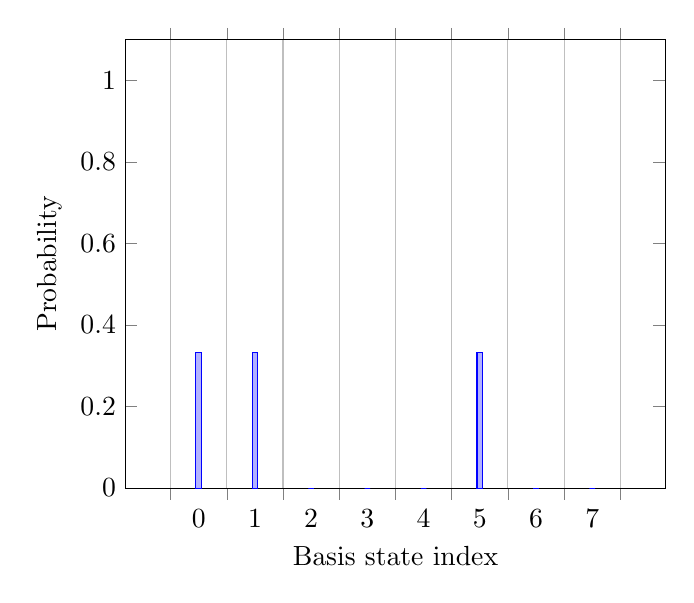
\begin{tikzpicture}
			\begin{axis}[
				ylabel = Probability,
				xlabel = Basis state index,
				ymin = 0,
				ymax = 1.1,
				ybar,
				ybar interval=0.1
			]
			\addplot 
				coordinates {(0,0.333333333333) (1,0.333333333333) (2,0) (3,0) (4,0) (5,0.333333333333) (6,0 ) (7,0) (8,1)};
			\end{axis}
		\end{tikzpicture}
		\caption{Probability distribution for convolution of $\text{T}_a = 11000100$ and $\overline{\text{P}}_a = 10000000$.}
		\label{fig:convolution-a}
	\end{figure}
	\begin{figure}
			\centering
			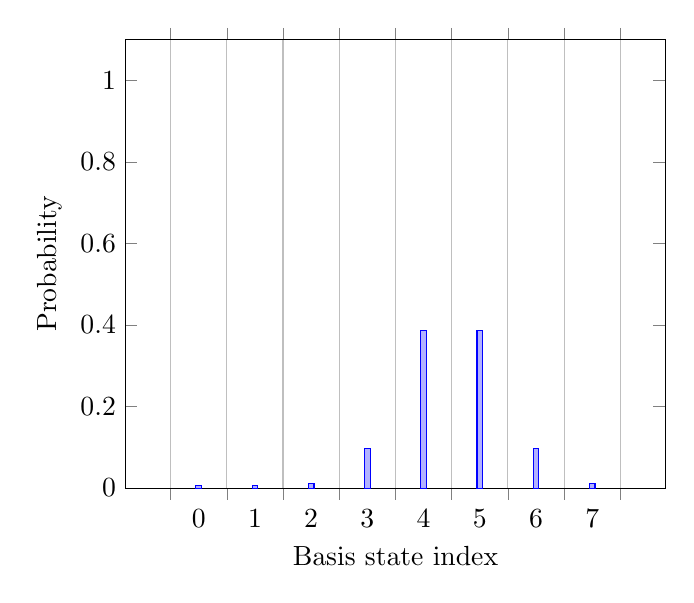
\begin{tikzpicture}
				\begin{axis}[
					ylabel = Probability,
					xlabel = Basis state index,
					ymin = 0,
					ymax = 1.1,
					ybar,
					ybar interval=0.1
				]
				\addplot 
					coordinates {(0,0.0055890168383) (1,0.0055890168383) (2,0.0107053460004) (3,0.0970357555674) (4,0.386669881594) (5,0.386669881594) (6,0.0970357555674 ) (7,0.0107053460004) (8,0)};
				\end{axis}
			\end{tikzpicture}
			\caption{Probability distribution for convolution of $\text{T}_b = 00111000$ and $\overline{\text{P}}_b = 01100000$.}
			\label{fig:convolution-b}
		\end{figure}
	
In Table~\ref{tab:convolution-a}, $0.333333333333 = \frac{1}{3}$ and $3.85185988877e^{-34} \approx 0$. Then, the only possible resulting values of a measurement operation on the current state of register $\alpha$ will be the indices 0, 1 and 5. These values correspond to the substrings $\text{T}_a[0, 0] = 1$, $\text{T}_a[0,1] = 11$ and $\text{T}_a[3,5] = 001$. In Table~\ref{tab:convolution-b}, the order of the indices in T according to probability of occurrence are as follows: 4 and 5, 3 and 6, 7 and 2, and lastly 1 and 0.
\end{example}

\begin{lemma}\label{lem:quantum-convolution-approximate}
	Algorithm~\ref{alg:qca} computes an approximation of the convolution of two binary sequences $\binseq{x}{\sigma}, \binseq{y}{\sigma}$ up to a global multiplicative factor
	\[
		\frac{1}{\sqrt{t_{\mathrm{x}}t_{\mathrm{y}}}}
	\]
and local multiplicative factor
	\[
		\frac{1}{\left\vert \frac{1}{\sqrt{L}}\frac{1}{\sqrt{\binseq{t}{x}}} \sum_{i=0}^{L-1} w^{ij}\binseq{x}{\sigma}[i] \right\vert}
	\]
where $t_{\mathrm{x}}, t_{\mathrm{y}}$ corresponds to the number of 1s in $\binseq{x}{\sigma}, \binseq{y}{\sigma}$, respectively, and $w^{ij}=e^{2\pi i \frac{ij}{L} }$ for all $j=0,\ldots,L-1$.
\end{lemma}

\begin{proof}
Operators $F$ and $F_{\mathrm{Q}}$ have the same unitary matrix representation given by
	\[
		F(i,j) = F_{\mathrm{Q}}(i,j) = \frac{1}{\sqrt{L}} w^{ij}
	\]
	for all $i,j=0,\ldots,L-1$. Same is true with their inverses,
	\[
		F^{-1}(i,j) = F_{\mathrm{Q}}(i,j) = \frac{1}{\sqrt{L}} w^{-ij}
	\]
for all $i=0,\ldots,L-1$. In the quantum setting, $\binseq{x}{\sigma}, \binseq{y}{\sigma}$ have a multiplicative factor of $\frac{1}{\sqrt{t_{\mathrm{x}}}}, \frac{1}{\sqrt{t_{\mathrm{y}}}}$, respectively. Step 1 of Algorithm~\ref{alg:qca} will transform $\binseq{x}{\sigma},\binseq{y}{\sigma}$ into sequences given by
\begin{align*}
	\langle j \myket{\binseq{X}{\sigma}} &= \langle j \vert \fq{\myket{\binseq{x}{\sigma}}}\\
	                                                        &= \frac{1}{\sqrt{L}} \frac{1}{\sqrt{t_{\mathrm{x}}}} \sum_{i=0}^{L-1} w^{ij} \binseq{x}{\sigma}[i]\\
	\langle j \myket{\binseq{Y}{\sigma}} &= \langle j \vert \fq{\myket{\binseq{y}{\sigma}}}\\
	                                                        &= \frac{1}{\sqrt{L}} \frac{1}{\sqrt{t_{\mathrm{y}}}} \sum_{i=0}^{L-1} w^{ij} \binseq{y}{\sigma}[i].
\end{align*}
Step 2 of Algorithm~\ref{alg:qca} corresponds to the point-wise multiplication step of the classical convolution algorithm and will transform $\myket{\binseq{X}{\sigma}}, \myket{\binseq{Y}{\sigma}}$ into the sequence given by
\begin{align*}
	\langle j \vert \V{X}{\binseq{Y}{\sigma}} = \frac{1}{L} \frac{1}{\sqrt{\binseq{t}{x}\binseq{t}{y}}} \left(\frac{\sum_{i=0}^{L-1} w^{ij} \binseq{x}{\sigma}[i]}{\left\vert \frac{1}{\sqrt{L}}\frac{1}{\sqrt{\binseq{t}{x}}} \sum_{i=0}^{L-1} w^{ij} \binseq{x}{\sigma}[i] \right\vert}\right)\left( \sum_{i=0}^{L-1} w^{ij} \binseq{y}{\sigma}[i] \right)
\end{align*}
for all $j=0,\ldots,L-1$. At this point, the quantum convolution algorithm already differs from the classical convolution algorithm by a global multiplicative factor of 
\[
	\frac{1}{\sqrt{\binseq{t}{x}\binseq{t}{y}}}
\] 
and a local multiplicative factor of
\[
	\frac{1}{\left\vert \frac{1}{\sqrt{L}} \frac{1}{\sqrt{\binseq{t}{x}}} \sum_{i=0}^{L-1} w^{ij} \binseq{x}{\sigma}[i] \right\vert}
\]
for all $j=0,\ldots,L-1$.
\end{proof}
%We constructively go through each step of the quantum convolution algorithm and compare the resulting states to that of the classical convolution algorithm. Let the binary indicator sequences $S_1= \alpha_0,\ldots,\alpha_{2^n-1}$ and $S_2=\beta_0,\ldots,\beta_{2^n-1}$ be the input sequences to the Classical convolution algorithm with respect to the symbol $\sigma \in \Sigma$. Let the quantum states
%	\[
%		\vert \alpha_{\sigma} \rangle_0 = \sqrt{\frac{1}{c_\sigma^\text{T}}} \sum_{i=0}^{2^n-1} \alpha_i \vert i \rangle
%	\] 
%	and
%	\[
%		\vert \beta_{\sigma} \rangle_0 = \sqrt{\frac{1}{c_\sigma^{\overline{\text{P}}}}} \sum_{i=0}^{2^n-1} \beta_i \vert i \rangle
%	\] 
%	be the quantum state encoding of the binary indicator sequences $S_1$ and $S_2$. These states will serve as input into the quantum convolution algorithm. $c_\sigma^\text{T}$ and $c_\sigma^{\overline{\text{P}}}$ corresponds to the number of occurrences of symbol $\sigma$ in T and $\overline{\text{P}}$, respectively.
%	
%Step 1 of the classical convolution algorithm results to a vector $X^1$ of values defined such that the \textit{i}-th element of the vector is defined as
%	\begin{align*}
%		X^1_i = \sqrt{\frac{1}{2^n}} \sum_{j=0}^{2^n-1} w^{ij} \alpha_j
%	\end{align*}
%Step 1 of the quantum convolution algorithm results to a quantum superposition state $\vert \alpha_{\sigma} \rangle_1$ defined such that
%	\begin{align*}
%		\langle i \vert \alpha_{\sigma} \rangle_1 = \sqrt{\frac{1}{2^n}} \sqrt{\frac{1}{c_\sigma^\text{T}}} \sum_{j=0}^{2^n-1} w^{ij} \alpha_j
%	\end{align*}
%Step 2 of the classical convolution algorithm will result to a new vector $X^2$ such that its elements are defined as
%	\begin{align*}
%		X^2_i = \sqrt{\frac{1}{2^n}} \sum_{j=0}^{2^n-1} w^{ij} \beta_j
%	\end{align*}
%Step 2 of quantum convolution algorithm will result to a quantum superposition state $\vert \beta_{\sigma} \rangle_1$ defined such that
%	\begin{align*}
%		\langle i \vert \beta_{\sigma} \rangle_1 = \sqrt{\frac{1}{2^n}} \sqrt{\frac{1}{c_\sigma^{\overline{\text{P}}}}} \sum_{j=0}^{2^n-1} w^{ij} \beta_j
%	\end{align*}
%Step 3 of the classical convolution algorithm will result to a vector $Y$ with values defined as
%	\begin{align*}
%		Y_i = \frac{1}{2^n}  \left( \sum_{j=0}^{2^n-1} w^{ij} \alpha_j \right) \left( \sum_{j=0}^{2^n-1} w^{ij} \beta_j \right)
%	\end{align*}
%Step 3 of the quantum convolution algorithm will result to a quantum superposition state $\vert \alpha_{\sigma} \rangle_2$ defined such that
%	\begin{align*}
%		\langle i \vert \alpha_{\sigma} \rangle_2 = \frac{1}{2^n} \sqrt{\frac{1}{c_\sigma^{\overline{\text{P}}}}} \sqrt{\frac{1}{c_\sigma^\text{T}}} \frac{ \left( \sum_{j=0}^{2^n-1} w^{ij} \alpha_j \right) \left( \sum_{j=0}^{2^n-1} w^{ij} \beta_j \right) }{ \bigg\vert \sqrt{\frac{1}{c_\sigma^{\overline{\text{P}}}}} \sum_{j=0}^{2^n-1} w^{ij} \alpha_j \bigg\vert }
%	\end{align*}
%The complex amplitudes in the resulting state $\vert \alpha_{\sigma} \rangle_2$ differs from the elements of vector $Y$ by a multiplicative factor
%	\begin{align*}
%		\sqrt{\frac{1}{c_\sigma^{\overline{\text{P}}}}} \sqrt{\frac{1}{c_\sigma^\text{T}}} \frac{1}{\bigg\vert \sqrt{\frac{1}{c_\sigma^{\overline{\text{P}}}}} \sum_{j=0}^{2^n-1} w^{ij} \alpha_j \bigg\vert}
%	\end{align*}
%Step 4 of the classical convolution algorithm will result to a vector $Z$ of elements defined such that
%	\begin{align}
%		\label{eqn:classical-convolution-algorthim-step-4}
%		Z_k &= \frac{1}{2^n} \sqrt{\frac{1}{2^n}} \sum_{l=0}^{2^n-1} w^{-kl} \sum_{i=0}^{2^n-1} \left( \sum_{j=0}^{2^n-1} w^{ij} \alpha_j \right) \left( \sum_{j=0}^{2^n-1} w^{ij} \beta_j \right)\\
%		&= \frac{1}{2^n} \sqrt{\frac{1}{2^n}} \sum_{j=0}^{2^n-1} \alpha_j \beta_{i-j}
%	\end{align}
%for $k = 0, \ldots, N+M-1$.	 Step 5 of the classical convolution algorithm will result to a vector $C$ with elements defined as
%	\begin{align}
%		C_i = \sum_{j=0}^{2^n-1} \alpha_j \beta_{i-j}
%	\end{align}
%Vector $C$ is the convolution of sequences $S_1$ and $S_2$. Step 4 of the quantum convolution algorithm transforms the state of the quantum register from state $\vert \alpha_\sigma \rangle_2$ into the quantum superposition state $\vert \alpha_{\sigma} \rangle_3$ defined such that
%	\begin{align}
%		\label{eqn:quantum-convolution-algorthim-step-4}
%		\langle k \vert \alpha_{\sigma} \rangle_3 = \frac{1}{2^n} \sqrt{\frac{1}{2^n}} \sqrt{\frac{1}{c_\sigma^{\overline{\text{P}}}}} \sqrt{\frac{1}{c_\sigma^\text{T}}} \sum_{l=0}^{2^n-1} w^{-kl} \Bigg( \sum_{i=0}^{2^n-1} \frac{ \left( \sum_{j=0}^{2^n-1} w^{ij} \alpha_j \right) \left( \sum_{j=0}^{2^n-1} w^{ij} \beta_j \right) }{ \bigg\vert \sqrt{\frac{1}{2^n}} \sqrt{\frac{1}{c_\sigma^{\overline{\text{P}}}}} \sum_{j=0}^{2^n-1} w^{ij} \alpha_j \bigg\vert } \Bigg)
%	\end{align}
%Based from Equations~\ref{eqn:classical-convolution-algorthim-step-4} and \ref{eqn:quantum-convolution-algorthim-step-4}, the quantum convolution algorithm approximates the classical convolution of two binary sequences of up to an overall normalizing multiplicative factor
%	\begin{align*}
%		\sqrt{\frac{1}{c_{\sigma}^{\overline{\text{P}}}}}\sqrt{\frac{1}{c_{\sigma}^{\text{T}}}}
%	\end{align*}
%and a local normalizing factor
%	\begin{align*}
%		\frac{1}{\bigg\vert \sqrt{\frac{1}{2^n}} \sqrt{\frac{1}{c_\sigma^{\overline{\text{P}}}}} \sum_{j=0}^{2^n-1} w^{ij} \alpha_j \bigg\vert}
%	\end{align*}
%These multiplicative factors are necessary to qualify the computation of the quantum convolution algorithm as a valid quantum computation.
%\end{proof}

%AQC makes use of a different encoding scheme as compared to what is used in the classical setting as presented in Section~\ref{sec:cc-encoding} due to some limitations resulting from requirements for a quantum system. Instead, it makes use of binary indicator sequences to encode T and P with respect to each symbol in $\Sigma$ (Section~\ref{subsec:binary-indicator-vectors}). Also, since the input to the problem is in classical encoding there is an additional quantum encoding step prior execution of AQC (Section~\ref{subsec:aqc-encoding}). This is of course common to quantum algorithms since input data to these algorithms are necessarily encoded into quantum memory registers prior to actual computation. 

%========== Consider adding to Appendix
%In the classical setting we encode the input strings T and P into sequences of 1s and -1s by using some functions $f(\cdot)$ and $g(\cdot)$. 
%
%\begin{example}
%\label{classical-encoding-example}
%	Given strings T = aabbba and P = bba and functions $f(\cdot)$ and $g(\cdot)$ defined such that
%	\begin{align*}
%		f(i) =
%		\begin{cases}
%			-1 & \text{ if } T[i] = a\\
%			1 & \text{ if } T[i] = b\\
%		\end{cases}
%		\ \ \text{ and }\ \
%		g(i) =
%		\begin{cases}
%			-1 & \text{ if } P[i] = a\\
%			1 & \text{ if } P[i] = b\\
%		\end{cases}
%	\end{align*}
%	the encoding of T with respect to $f(\cdot)$ is 
%	\begin{align*}
%		T^f &= f(0),f(1),f(2),f(3),f(4),f(5)\\
%				&= -1,-1,1,1,1,-1
%	\end{align*}
%	and the encoding of P with respect to $g(\cdot)$ is
%	\begin{align*}
%		P^g &= g(0),g(1),g(2)\\
%				&= 1,1,-1\ .
%	\end{align*}
%\end{example}
%
%Providing $T^f$ and $\overline{P^g}$ into the classical convolution algorithm and performing some final steps on the resulting values gives us a sequence of values corresponding to the number of matches of each candidate subsequence of T when compared against P. 
%
%\begin{example}
%	Given the encoding of T and $\overline{P}$ in Example~\ref{classical-encoding-example} and providing them as input to classical convolution algorithm, the resulting sequence of values will be the corresponding number of matches less number of mismatches for each valid subsequence of T,
%	\begin{align*}
%		Z &= 1 - 0, 1 - 1, 0 - 3, 1 - 2, 2 - 1, 3 - 0, 1 - 1, 0 - 0\\
%			&= 1, 0, -3, -1, 1, 3, 0, 0
%	\end{align*}
%	Adding $M=3$ to each value and dividing each resulting value with 2 will result to a sequence of values corresponding to the number of matches for each subsequence of T,
%	\begin{align*}
%		C &= \frac{1+3}{2},\frac{0+3}{2}, \frac{-3+3}{2}, \frac{-1+3}{2}, \frac{1+3}{2}, \frac{3+3}{2}, \frac{0+3}{2}, \frac{0+3}{2}\\
%			&= 2, 1\frac{1}{2}, 0, 1, 2, 3, 1\frac{1}{2}, 1\frac{1}{2}
%	\end{align*}
%\end{example}
%
%In the quantum setting we also need to encode first the input strings into a sequence of representative values so we can provide them as input into the AQC algorithm. One way of encoding data into quantum systems is to encode it into the amplitude of the quantum states of the system. The quantum operators which will be used in the AQC algorithm will be operating on the complex amplitudes and so encoding data into the amplitudes of quantum states instead of the quantum states will be more appropriate. Intuitively, we may just follow the encoding scheme we used in the classical setting for the quantum encoding which is to map the value $-1$ to the symbol '\textit{a}' and $1$ to the symbol '\textit{b}' via functions $f(\cdot)$ and $g(\cdot)$.
%\begin{example}
%	Given the encoding of T and P into $T^f$ and $P^g$ in Example \ref{classical-encoding-example} and adopting its encoding scheme for the quantum encoding of T and P we will have the following quantum states
%\begin{align*}
%	\vert \alpha \rangle = -\sqrt{\frac{1}{6}}\vert 000 \rangle -\sqrt{\frac{1}{6}}\vert 001 \rangle + \sqrt{\frac{1}{6}}\vert 010 \rangle + \sqrt{\frac{1}{6}}\vert 011 \rangle + \sqrt{\frac{1}{6}}\vert 100 \rangle - \sqrt{\frac{1}{6}}\vert 101 \rangle
%\end{align*}
%corresponding to $T^f$ and
%\begin{align*}
%	\vert \beta \rangle = -\sqrt{\frac{1}{3}} \vert 000 \rangle + \sqrt{\frac{1}{3}} \vert 001 \rangle + \sqrt{\frac{1}{3}} \vert 010 \rangle
%\end{align*}
%corresponding to $\overline{P^g}$.	
%\end{example}
%This encoding scheme though will not be of practical use for the AQC algorithm as detailed in Appendix \ref{app:encoding}. Instead, we use a different encoding scheme which is also often used in the classical setting.
%
%We use a new set of functions $F(\cdot)$ and $G(\cdot)$ for the quantum encoding of T and P defined such that
%%\begin{align*}
%%	F(i) = 
%%	\begin{cases}
%%		
%%	\end{cases}
%%\end{align*}
%
%\begin{example}
%	
%\end{example}
%
%Since we are only considering binary alphabets
%
%In the classical setting we encode each symbol of T and P as the state of a set of distinct bits. The encoding of T and P are then sequences of states of distinct sets of bits.  

%================================

%%%%%%%%%%%%%%%%%%%%%%%%% Correctness of Result %%%%%%%%%%%%%%%%%%%%%%%%%
%\note{Consider removing this section. Proof of correctness is by construction.}
%\section{Correctness of Result}
%\label{sec:correctness}
%The classical algorithm for approximate string matching which makes use of the convolution method provides as output a classical register of size $N+M-1$ with data at each index $i \in \{~0~,~\ldots~,~N~+~M~-~2~\}$ as
%
%\[
%	M - d\left(P, T[i, i+M-1] \right)
%\]
%which is the number of matches between P and the substring $\text{T}[i, \ldots, i+M-1]$. This algorithm provides all the solution in a single iteration. On the other hand, since QASM makes use of quantum memory registers for data storage, only a single index $i \in \{0, \ldots, N~+~M~-~2~\}$ will result from a single execution of the quantum algorithm and thus the need for several iterations.
%
%For the execution of sub-routine AQC for each symbol $\sigma \in \Sigma$ in Step~\ref{alg:qasm:step:aqc} of Algorithm~\ref{alg:qasm} the expected number of iterations in order for a substring $T_\sigma[i,i+M-1]$ of the binary indicator sequence $T_\sigma$ to be included into set $C_\alpha$ is
%\begin{align}
%	\frac{1}{\vert \langle i \vert \alpha_{b_3} \rangle \vert^2}
%\end{align}
%This shows that substrings of the binary indicator sequences $T_\sigma$ with greater number of matches compared to P will require less expected number of iterations to come out as result of measurement in Step~\ref{alg:qasm:step:M} of Algorithm~\ref{alg:qasm} and then to be included into set $C_\sigma$.

\subsection{Verification of classical result}\label{subsec:verification-classical-result}
For each iteration \textit{j} of Algorithm~\ref{alg:qca} we measure each quantum superposition state $\myket{\binseq{z}{\sigma_i}}$ to get a classical value $z_{\sigma_{i}}^j \in \{0,\ldots,N+M-1\}$, for $i=\{0,\ldots,L-1\}$. We record each resulting classical value $z_{\sigma_{i}}^j$ in a table $A_{\mathrm{T},\mathrm{P}}$ as described in Table~\ref{tab:A_matrix}. Recall function $g:\Sigma \rightarrow \{0,\ldots,M-1\}$ defined in Section~\ref{sec:application-to-approximate-string-matching}. Table $A_{\mathrm{T},\mathrm{P}}$ is defined such that
\[
	A_{\mathrm{T},\mathrm{P}}(i,j) = z_{\sigma_{i}}^j - g(\sigma_i)
\]
for all $i=1,\ldots,\vert \Sigma \vert$ and $j=1,\ldots,K$. We record the unique values in $A_{\mathrm{T},\mathrm{P}}$ where $M-1 \leq A_{\mathrm{T},\mathrm{P}}(i,j) \leq N-M+1$ in an ordered set $B_{\mathrm{T},\mathrm{P}}$, from highest to lowest number of occurrence in $A_{\mathrm{T},\mathrm{P}}$.

Each element in $B_{\mathrm{T},\mathrm{P}}$ can be verified classically by checking if
\[
	H\left( \mathrm{P}, \mathrm{T}[B_{\mathrm{T},\mathrm{P}}(i)],\ldots,\mathrm{T}[B_{\mathrm{T},\mathrm{P}}(i) + M - 1] \right) \leq d
\]
for all $i=1,\ldots,K$. Classical verification can be performed in $\Om\left( M \right)$ time steps.

%%%%%%%%%%%%%%%%%%%%%%%%% QASM algorithm %%%%%%%%%%%%%%%%%%%%%%%%%
\section{Quantum algorithm 2}\label{sec:quantum-algorithm-2}
In Algorithm~\ref{alg:convolution-based-quantum-algorithm} we define an algorithm which makes use of the ESQUID algorithm and quantum convolution algorithm for solving the approximate string matching problem. We let $Sol = \{ \}$ initially.

%Given the sub-routines presented in the previous sections, Quantum algorithm 2 is defined in Algorithm~\ref{alg:quantum-algorithm-2}.
\begin{algorithm}
	\caption{Convolution-based quantum algorithm for approximate string matching}
	\label{alg:convolution-based-quantum-algorithm}
	\begin{algorithmic}[1]
		\REQUIRE{text $\mathrm{T} \in \Sigma^N$, pattern $\mathrm{P} \in \Sigma^M$, Hamming distance constraint \textit{d}}
		\ENSURE{set of indices \textit{i} such that $H(\mathrm{P},\mathrm{T}[i],\ldots,\mathrm{T}[i+M-1]) \leq d$}
		\FOR{ j=1,\ldots,K}
			\FORALL {$\sigma_i \in \Sigma$}
				\STATE $\myket{\binseq{T}{\sigma_i}} = \mathrm{ESQUID}(\binseq{T}{\sigma_i})$
				\STATE $\myket{\binseq{P}{\sigma_i}} = \mathrm{ESQUID}(\binseq{P}{\sigma_i})$
				\STATE $\myket{\binseq{z}{\sigma_i}} = \mathrm{QCON}(\myket{\binseq{T}{\sigma_i}},\myket{\binseq{P}{\sigma_i}})$
				\STATE $\mathrm{z}^j_{\sigma_i} = \mathrm{M}\left( \myket{z_{\sigma_i}} \right)$
				\STATE $A_{\mathrm{T},\mathrm{P}}(i,j) = g(\sigma_i) - \mathrm{z}^j_{\sigma_i}$
			\ENDFOR
		\ENDFOR
		\STATE Construct $B_{\mathrm{T},\mathrm{P}}$ from $A_{\mathrm{T},\mathrm{P}}$.
		\FORALL {$i \in B_{\mathrm{T},\mathrm{P}}$}
			\IF {$H\left( \mathrm{P}, \mathrm{T}[i],\ldots,T[i + M - 1] \right) \leq d $}
				\STATE $Sol \cup \{i\}$
			\ENDIF
		\ENDFOR
		\RETURN \textit{Sol}
		
%		\STATE Encode T and P into binary indicator sequences $\text{T}_a$, $\overline{\text{P}}_a$, $\text{T}_b$ and $\overline{\text{P}}_b$ using sub-routine CEncode(T,P).
%		\FOR{$i=0$ to $j$}
%			\FOR{\textbf{each} $\sigma \in \Sigma=\{a,b\}$ }
%				\STATE Encode $\text{T}_{\sigma}$ and $\overline{\text{P}}_{\sigma}$ into the state of quantum registers QRegT and QRegP respectively using sub-routine ESQUID($\vert \psi_{map} \rangle$). \label{alg:qasm:qencode}
%				\STATE Perform convolution on the state of QRegT and QRegP using sub-routine AQC($\vert \alpha_\sigma \rangle$,~$\vert \beta_\sigma \rangle$). \label{alg:qasm:step:aqc}
%				\STATE Measure the state of QRegT. \label{alg:qasm:step:M}
%				\STATE Add resulting classical value \textit{k} less $\left(M-1\right)$ to set $C_{\sigma}$.
%			\ENDFOR
%		\ENDFOR
%		\STATE Get the union of sets $C_a$ and $C_b$, $C=C_a \cup C_b$.
%		\FOR{\textbf{each} $i \in C$}
%			\IF{ $d(\text{T}[i,i+M-1],\text{P}) \leq D$ }
%				\STATE Add \textit{i} to $C^\prime$
%			\ENDIF
%		\ENDFOR
%		\STATE Return $C^\prime$
	\end{algorithmic}
\end{algorithm}

\begin{theorem}
There exists a quantum algorithm which outputs \textit{k} starting indices of approximate copies $\mathrm{T}[i],\ldots,\mathrm{T}[i+M-1]$ of P in T in time complexity
\[
	\Om\left( K\left(\log_2^2 L + q\log_2 L\right)\right)
\]
with each index having the probability
\[
   \prod_{\sigma \in \Sigma} \left\vert \frac{1}{L\sqrt{L}}\frac{1}{\sqrt{t^{\mathrm{T}}_{\sigma}t^{\mathrm{P}}_{\sigma}}}  \left[ \sum_{j=0}^{L-1} w^{-jl} \left[ \left(\frac{\sum_{i=0}^{L-1} w^{ij}\cdot\mathrm{T}_{\sigma}[i]}{\left\vert \frac{1}{\sqrt{L}}\frac{1}{\sqrt{t^{\mathrm{T}}_{\sigma}}} \sum_{i=0}^{L-1} w^{ij}\cdot\mathrm{T}_{\sigma}[i] \right\vert}\right)\left( \sum_{i=0}^{L-1} w^{ij}\cdot\mathrm{P}_{\sigma}[i]\right)  \right] \right] \right\vert^2
\]
where $L=N+M-, q \ll L, k \ll K, w^{\pm jl}=e^{\pm 2\pi i j\frac{l}{L}}$, and $t^{\mathrm{T}}_{\sigma}, t^{\mathrm{P}}_{\sigma}$ is the number of occurrence of symbol $\sigma$ in the binary indicator sequence $\mathrm{T}_{\sigma}$ and $\mathrm{P}_{\sigma}$ respectively.
\end{theorem}
\begin{proof}
By Lemma~\ref{lem:quantum-convolution-time-complexity}, the computed total time complexity of computing for the convolution of two binary indicator sequences $\mathrm{T}_{\sigma}$ and $\mathrm{P}_{\sigma}$, $\sigma \in \Sigma$ is 
\[
	\Om\left( \log_2^2 L + q\log_2 L \right).
\]
In Section~\ref{sec:time-space-complexity}, the number of iterations of the quantum convolution algorithm is bounded as
\[
	K \in \Om\left(\frac{L\log_2 L + L}{\log_2^2 L + q\log_2 L}\right)
\]
By Lemma~\ref{lem:quantum-convolution-approximate}, each state $\vert l \rangle$ in the quantum convolution of the pair of binary indicator sequences $\mathrm{T}_{\sigma}, \mathrm{P}_{\sigma}$ has amplitude
\[
	\frac{1}{L\sqrt{L}}\frac{1}{\sqrt{t^{\mathrm{T}}_{\sigma}t^{\mathrm{P}}_{\sigma}}}  \left[ \sum_{j=0}^{L-1} w^{-jl} \left[ \left(\frac{\sum_{i=0}^{L-1} w^{ij}\cdot\mathrm{T}_{\sigma}[i]}{\left\vert \frac{1}{\sqrt{L}}\frac{1}{\sqrt{t^{\mathrm{T}}_{\sigma}}} \sum_{i=0}^{L-1} w^{ij}\cdot\mathrm{T}_{\sigma}[i] \right\vert}\right)\left( \sum_{i=0}^{L-1} w^{ij}\cdot\mathrm{P}_{\sigma}[i]\right)  \right] \right].
\]
The probability of getting an index \textit{l} as starting index of an approximate copy of P in T is then the product of the probabilities of getting \textit{k} as classical result of measuring the quantum convolution of binary indicator sequences $\mathrm{T}_{\sigma}$ and $\mathrm{P}_{\sigma}$ for all $\sigma \in \Sigma$, which is given by
\[
   \prod_{\sigma \in \Sigma} \left\vert \frac{1}{L\sqrt{L}}\frac{1}{\sqrt{t^{\mathrm{T}}_{\sigma}t^{\mathrm{P}}_{\sigma}}}  \left[ \sum_{j=0}^{L-1} w^{-jl} \left[ \left(\frac{\sum_{i=0}^{L-1} w^{ij}\cdot\mathrm{T}_{\sigma}[i]}{\left\vert \frac{1}{\sqrt{L}}\frac{1}{\sqrt{t^{\mathrm{T}}_{\sigma}}} \sum_{i=0}^{L-1} w^{ij}\cdot\mathrm{T}_{\sigma}[i] \right\vert}\right)\left( \sum_{i=0}^{L-1} w^{ij}\cdot\mathrm{P}_{\sigma}[i]\right)  \right] \right] \right\vert^2
\]
\end{proof}

%Since any quantum computation only returns a single classical value at the end of its computation, the quantum sub-routines ESQUID and AQC needs to be invoked multiple times. Also, since we encode the classical input T and the reverse of P into binary indicator sequences, we need to execute ESQUID and AQC for each encoding of T and P with respect to each symbol $\sigma \in \Sigma$. 

%ESQUID and AQC sub-routines can be performed in parallel for each symbol $\sigma$ though. We need to allocate $2\vert \Sigma \vert$ quantum memory registers to accommodate the input data.
%\begin{example}
%\label{exa:qasm}
%	Given input strings $\text{T}= aabbba$ and $\text{P}= bba$ and Hamming distance constraint $\text{D}=2$ we invoke QASM as $\text{QASM}(aabbba, bba, 2)$. CEncode(T,P) will encode T and P with respect to symbols '\textit{a}' and '\textit{b}' as $\text{T}_a = 110001$, $\text{T}_b = 001110$, $\overline{\text{P}}_a = 100$ and $\overline{\text{P}}_b = 011$. ESQUID will encode $\text{T}_a$, $\overline{\text{P}}_a$, $\text{T}_b$ and $\overline{\text{P}}_b$ into quantum superposition states
%	\begin{align*}
%		\vert \alpha_a \rangle &= \sqrt{\frac{1}{3}}\vert 000 \rangle + \sqrt{\frac{1}{3}}\vert 001 \rangle + \sqrt{\frac{1}{3}}\vert 101 \rangle\ ,\\
%		\vert \beta_a \rangle &= \vert 000 \rangle\ ,\\
%		\vert \alpha_b \rangle &= \sqrt{\frac{1}{3}}\vert 010 \rangle + \sqrt{\frac{1}{3}}\vert 011 \rangle + \sqrt{\frac{1}{3}}\vert 100 \rangle\ ,\\
%		\vert \beta_b \rangle &= \sqrt{\frac{1}{2}}\vert 000 \rangle + \sqrt{\frac{1}{2}}\vert 001 \rangle
%	\end{align*}
%	respectively. AQC will then be invoked both for symbol '\textit{a}' and '\textit{b}'. Invoking $\text{AQC}(\vert \alpha_a \rangle, \vert \beta_a \rangle)$ will result to the quantum superposition state
%	\begin{align*}
%		\vert \tau_a \rangle &\approx K_a \left( 1\cdot \vert 000 \rangle + 1\cdot \vert 001 \rangle + 0\cdot \vert 010 \rangle + 0\cdot \vert 011 \rangle + 0\cdot \vert 100 \rangle + 1\cdot \vert 101 \rangle + 0\cdot \vert 110 \rangle + 0\cdot \vert 111 \rangle \right)\\
%		&\approx K_a\left( \vert 000 \rangle + \vert 001 \rangle + \vert 101 \rangle \right)
%	\end{align*}
%	where
%	\[	
%		K_a = \frac{1}{8}\sqrt{\frac{1}{8}}\sqrt{\frac{1}{3 \cdot 1}}
%	\]
%	and $\text{AQC}(\vert \alpha_b \rangle, \vert \beta_b \rangle)$ to
%	\begin{align*}
%		\vert \tau_b \rangle &\approx K_b\left( 0\cdot\vert 000 \rangle + 0\cdot\vert 001 \rangle + 0\cdot\vert 010 \rangle + 1\cdot\vert 011 \rangle + 2\cdot \vert 100 \rangle + 2\cdot\vert 101 \rangle + 1\cdot\vert 110 \rangle + 0\cdot\vert 111 \rangle \right)\\
%		&\approx K_b\left( \vert 011 \rangle + 2\vert 100 \rangle + 2\vert 101 \rangle + \vert 110 \rangle \right)
%	\end{align*}
%	where
%	\[	
%		K_b = \frac{1}{8}\sqrt{\frac{1}{8}}\sqrt{\frac{1}{3 \cdot 2}}\ .
%	\]
%Classical values $-2, -1$ and $3$, corresponding to indices $000=0, 001=1$ and $101=5$ less $(M-1)$, all have the probability of
%	\begin{align*}
%		&\approx \vert K_a \cdot 1 \vert^2\\
%		&\approx \Bigg\vert \frac{1}{8}\sqrt{\frac{1}{8}}\sqrt{\frac{1}{3 \cdot 1}} \cdot 1 \Bigg\vert^2
%	\end{align*}		
%of being included into the set $C_a$.	Classical values $1$ and $4$, corresponding to indices $011=3$ and $110=6$ less $(M-1)$, have the probability of
%	\begin{align*}
%		&\approx \vert K_b \cdot 1 \vert^2\\
%		&\approx \Bigg\vert \frac{1}{8}\sqrt{\frac{1}{8}}\sqrt{\frac{1}{3 \cdot 2}} \cdot 1 \Bigg\vert^2
%	\end{align*}
%while values $2$ and $3$, corresponding to indices $100=4$ and $101=5$ less $(M-1)$, have probability
%	\begin{align*}
%		&\approx \vert K_b \cdot 2 \vert^2\\
%		&\approx \Bigg\vert \frac{1}{8}\sqrt{\frac{1}{8}}\sqrt{\frac{1}{3 \cdot 2}} \cdot 2 \Bigg\vert^2
%	\end{align*}
%of being included into the set $C_b$. \note{what is optimal value for j?} After some number of iterations \textit{j} we expect to have the set of indices $C^\prime=\{-2,-1,1,2,3,4\}$ where negative values correspond to comparisons in which P is extended to the left of T starting from alignment of $\text{T}[0]$ with $\text{P}[M-1]$. Positive values greater than $N-M+1$ correspond to comparisons in which P is extended to the right of T ending with alignment of $\text{T}[N-1]$ with $\text{P}[0]$. The elements of set $C^\prime$ correspond to the sub-sequences $a$, $aa$, $abb$, $bbb$, $bba$ and $ba$ respectively. When compared with $\text{P}=bba$ these sub-sequences have $2, 2, 2, 1, 0, 2$ number of mismatches, respectively.
%\end{example}

%%%%%%%%%%%%%%%%%%%%%%%%% Time and Space Complexity %%%%%%%%%%%%%%%%%%%%%%%%%
%\section{Time and Space Complexity}
%\label{sec:complexity}
%We compute for the time and space complexity of the sub-routines of Quantum algorithm 2 to compute for its overall complexity. 
%
%The construction of the superposition quantum states representing the strings T and reverse of P, both padded with 0s, using the ESQUID sub-routine will require time complexity $O(\log_2{\left(N+M\right)})$ and space complexity of $O(\log_2{\left(N+M\right)})$. In the AQC algorithm, the \textit{QFT} steps will require $O(\log_2^2{\left(N+M\right)})$ time complexity while the approximation of the dot multiplication step will require $O(N+M)$ time complexity. The linear time complexity for the approximation of the dot multiplication step can be attributed to the resource-intensive implementation of diagonal unitary matrices on quantum circuits using only one- and two-qubit quantum gates. An efficient algorithm for implementing diagonal unitaries without ancilla qubits on quantum circuits can be found in \cite{Welch2014}. The execution of the AQC sub-routine can be done in parallel to compensate for the $\vert \Sigma \vert$ multiplicative factor. The space complexity of the AQC sub-routine is $O(\log_2{\left( N+M \right)})$ since we need to allot quantum registers for both T and the reverse of P. The last loop in Quantum algorithm 2 verifies the found indices in T if they satisfy the input distance requirement and is bounded above by the number of iterations $j$ in the previous loop in Quantum algorithm 2.  
%
%Note that Quantum algorithm 2 is advantageous with regards to computation time steps in comparison to the classical algorithm which uses convolution method if it is the case that 
%\begin{align}
%\label{constraint-on-j}
%	j < \log_2{\left( N+M \right)} \ .
%\end{align}
%where $j$ is bounded above by the number of substrings of T starting at position $i$ and satisfying the distance constraint
%\[
%	d\left(\text{P}, \text{T}[i, i+M-1] \right) \leq D
%\]
%From this we see that the improvement on the time complexity by the Quantum algorithm 2 in comparison to that of Algorithm~\ref{alg:cc} is a reduction from \textit{log}-\textit{linear} to \textit{linear} time steps, with the assumption that the condition \ref{constraint-on-j} is satisfied. 
%\note{Compute for probability of success.}

%\section{Limitations}
%\label{sec:limitations}

%\subsection{Totally no occurrence of P in T}

%%%%%%%%%%%%%%%%%%%%%%%%% Simulation %%%%%%%%%%%%%%%%%%%%%%%%%
%\section{Simulation}

\section{Summary}
In this chapter we presented the concept of convolution and how it applies to the problem of approximate string matching, both in the classical and quantum setting. We presented a convolution-based quantum algorithm for approximate string matching defined in Algorithm~\ref{alg:convolution-based-quantum-algorithm}. It encodes the input strings T and P into binary indicator sequences for all symbols $\sigma \in \Sigma$. These binary indicator sequences are prepared as quantum superposition states which serve as input to the quantum convolution algorithm in Algorithm~\ref{alg:qca}. The algorithm uses ESQUID algorithm \cite{Rosenbaum2009} for generating the quantum superposition state encoding of the binary indicator sequences for T and P. ESQUID algorithm has circuit and time complexity bounded by $\Om\left( \log_2 L \right)$. It uses the same binary indicator sequence registers used all through the algorithm plus two additional ancillary qubits for coding the progress of its state generation process. Its time complexity is in $\Om\left( \log_2 L \right)$.

We outlined the flow of the quantum convolution algorithm in Section~\ref{subsec:qft} and provided details about its sub-routines in Section~\ref{sec:sub-routines}. The quantum Fourier transform has been shown to be exactly implementable in a quantum circuit with circuit depth of $\Om\left( \log_2^2 L + \log_2 L\right)$ in \cite{Shor2004}. Its circuit and time complexity is thus also bounded the same. It works on the same binary indicator sequence registers used in the ESQUID sub-routine and so works on $\log_2 L$ qubits. The same goes for its inverse. The classical point-wise multiplication operation was also implemented using a unitary diagonal matrix $V_\mathrm{X}$ based on the unitary matrix suggested in \cite{Curtis2004}. We introduced a minor revision of the values of $V_{\mathrm{X}}$ to accommodate the case where there exists states $\vert i \rangle$ in superposition state $\vert X \rangle$ which have an amplitude of zero. This is to avoid division by zero in $V_{\mathrm{X}}$. Using the same analysis for operator $W$ in the previous algorithm, we analyzed the the circuit complexity of a quantum circuit for $V_{\mathrm{X}}$ when decomposed using the Clifford+T gate set. The circuit complexity of $V_{\mathrm{X}}$ will be in $\left( \log_2 L \right)$ assuming $q \ll L$ where \textit{q} is the number of distinct phase values along the diagonal matrix of $V_{\mathrm{X}}$ Its time complexity will thus also be bounded the same. Operator $V_{\mathrm{X}}$ will also work on the same binary indicator sequences used in the previous steps.

Given ordered set $B_{\mathrm{T},\mathrm{P}}$, the resulting indices of the quantum convolution algorithm can be verified classically by checking if $H\left( \mathrm{P}, \mathrm{T}[i],\ldots,\mathrm{T}[i+M-1] \right) \leq d$. Parallelizing the verification of the elements of $B_{\mathrm{T},\mathrm{P}}$ by synthesizing a classical circuit of circuit complexity in $\Om\left(KM\log_2 \vert \Sigma \vert \right)$ will give the classical verification step time complexity in $\Om\left( 1 \right)$ only.

The convolution-based quantum algorithm for approximate string matching presented in this chapter has circuit complexity in
\[
	\Om\left( \log_2^2 L + q\log_2 L + KM\log_2 \vert \Sigma \vert \right),
\]
time complexity in
\[
	\Om\left( K\left(\log_2^2 L + q\log_2 L \right) \right),
\]
and space complexity in
\[
	\Om\left(\vert \Sigma \vert\log_2 L + KM\log_2 \vert \Sigma \vert \right).
\]








In the previous two chapters we presented quantum algorithms which tried to find exact or approximate copies of P in T in the whole search space $\{0,\ldots,N-1\}$. In this chapter we present a quantum algorithm for minimizing the search space by removing elements of the space which do not satisfy a specific criteria. We present a quantum algorithm for the approximate string matching problem which outputs an index \textit{i} in T satisfying the distance threshold requirement with probability directly proportional to the number of matching distinct symbols in P and the substring of T. We use the alphabet $\Sigma=\{a,b,c,d\}$, text $\text{T}= abccabcd$, pattern $\text{P}= abcd$, and distance threshold $d=1$ all throughout this chapter for illustration purposes.

\todo{list explicit contributions}

%The quantum algorithm presented in Chapter \ref{chapter:quantum-convolution} is better suited for instances of the approximate string matching problem in which the size of $\Sigma$ is small since the initial quantum superposition states need to be initialized for T and P for each symbol $\sigma \in \Sigma$. In this chapter we present a quantum algorithm which assumes a an alphabet of large size and a pattern P reach in symbols from $\Sigma$. We use the alphabet $\Sigma=\{a,b,c,d\}$, text $\text{T}= dcbcbaa$, pattern $\text{P}= cbad$ and distance threshold $d=1$ all through out this chapter for illustration purposes.

%%%%%%%%%%%%%%%%%%%%%%%%%%%%%%%%%% Filtering phase %%%%%%%%%%%%%%%%%%%%%%%%%%%%%%%%%%
%\section{Filtering phase}\label{sec:filtering-phase}
\section{Preliminary: A classical filtering algorithm}\label{subsec:filtering-phase-preliminaries}
A. Amir, M. Lewenstein and E. Porat in \cite{Amir2004} proposed a classical algorithm which minimizes the solution space of a string matching problem with specified number of mismatches. We use the following notation in order to explain the filtering concept in the classical algorithm of Amir et al. Let 
\begin{itemize}
	\item $\text{P}_{\Sigma} = \{\alpha_1,\alpha_2, \ldots, \alpha_{q}\}$, $\vert \mathrm{P}_{\Sigma} \vert = q$, set containing all distinct symbols in P
	\item $\text{P}_{\Sigma}^{2d} = $ set containing arbitrary 2\textit{d} elements of the set $\text{P}_{\Sigma}$
	\item $\gamma: \text{P}_{\Sigma} \rightarrow \{0,\ldots,M-1\}; \gamma(\alpha_{j}) = i$ such that $\alpha_{j} \neq \text{P}[k]$ for $0 \leq k < i < M$
\end{itemize}
$\gamma(\cdot)$ is a mapping between elements of $\text{P}_{\Sigma}$ and their index of first occurrence in P.
%We define two sets $P_{\mathrm{Sym}}$ and $P_{\mathrm{Loc}}$. Let $P_{\mathrm{Sym}}$ be the set of all distinct symbols in P. Let $P_{\mathrm{Loc}}$ be the set of indices of first occurrence in P of each symbol in $P_{\mathrm{Sym}}$.  Let both sets be totally ordered such that for any two symbols $x$ and $y$ in $P_{\mathrm{Sym}}$ and two indices $k$ and $l$ in $P_{\mathrm{Loc}}$, $x$ precedes $y$ in $P_{\mathrm{Sym}}$ and $k$ precedes $l$ in $P_{\mathrm{Loc}}$ only if $T[k]=x$, $T[l]=y$ and $k < l$. Let $\vert P_{\mathrm{Sym}} \vert = \vert P_{\mathrm{Loc}} \vert = q$. We denote the $i$-th symbol element of $P_{\mathrm{Sym}}$ to be $P_{\mathrm{Sym}_i}$ and the $i$-th element of $P_{\mathrm{Loc}}$ to be $P_{\mathrm{Loc}_i}$ for $1 \leq i \leq q$.
%substring
%Let $P_{\mathrm{Sym}}$ be the set of distinct symbols in P. Let $P_{\mathrm{Sym}}$ be a totally ordered set such that for any two symbols $P_{\mathrm{Sym}}(i)$, and $P_{\mathrm{Sym}}(j)$, symbol $P_{\mathrm{Sym}}(i)$ precedes symbol $P_{\mathrm{Sym}}(j)$ in set $P_{\mathrm{Sym}}$ only if $P[k]=P_{\mathrm{Sym}}(i), P[l]=P_{\mathrm{Sym}}(j)$ and $k < l$. Let $\vert P_{\mathrm{Sym}} \vert = q$. Let $P_{\mathrm{Loc}}$ be the set of location of first occurrence in P of each symbol in $P_{\mathrm{Sym}}$. Let $P_{\mathrm{Loc}}$ also be a totally ordered set. Given $P_{\mathrm{Sym}}$ and $P_{\mathrm{Loc}}$ we define a mapping $\phi: P_{\mathrm{Sym}} \rightarrow P_{\mathrm{Loc}}$ such that $\phi(P_{\mathrm{Sym}}(i)) = P_{\mathrm{Loc}}(i) \  \forall i, 1 \leq i \leq q$. We assume that $q \geq 2d$. In our example instance, $P_{\mathrm{Sym}}=\{a,b,c,d\}$ and $P_{\mathrm{Loc}}=\{0,1,2,3\}$, $q=4$. Mapping $\phi$ is defined such that $\phi(a)=0, \phi(a)=1, \phi(a)=2, \phi(a)=3$. 

%Let $A=\{\sigma_1, \sigma_2, \ldots, \sigma_q\}$ be a set of all distinct symbols in $\Sigma$ found in P. Let $\vert A \vert = q \geq 2d$. Also, let $A_{loc}=\{j_{\sigma_1}, j_{\sigma_2}, \ldots, j_{\sigma_q} \}$ be the set of locations in P corresponding to the distinct symbols in $A$ such that $P[i_{\sigma_k}] = \sigma_k$ and there exists no other location $0 \leq i < i_{\sigma_k}$ where $P[i] = \sigma_k$. In the quantum algorithm we assume that we can look into sets $A$ and $A_{loc}$ any time as databases in unit time step. Given P, set $A$ is defined to be the set $A=\{a,b,c,d\}$ and the set of locations of symbols in $A$ is defined to be the set $A_{loc}=\{2,1,0,3\}$. We see that $\vert A \vert = 4 $ and $\vert A \vert > 2d$.
In \cite{Amir2004} the elements of $\text{P}_{\Sigma}^{2d}$ is limited only to $2d$ distinct symbols in P. Given a symbol $\mathrm{T}[i]$ and index $\gamma(\mathrm{T}[i])$, index $(i - \gamma(\mathrm{T}[i]))$ in T indicates a possible starting location of P in T. We can slide through T starting at index 0 up to index \textit{N}-1 and evaluate and record the value $(i - \gamma(\mathrm{T}[i]))$ at each index \textit{i}. After the evaluation of each index \textit{i} in T, starting locations of occurrences of P in T will correspond to the most frequently occurring indices $(i - \gamma(\mathrm{T}[i]))$ in our record. We can imagine this process as having \textit{N} buckets labelled from $j=0,\ldots,N-1$ in which we drop a ball in bucket \textit{j} whenever $j=i-\gamma(\mathrm{T}[i])$. The label of the buckets with most number of balls will correspond to a probable starting location of an exact or approximate copy of P in T. Figure~\ref{fig:Amir-filtering-algorithm} illustrates how the classical algorithm of Amir et al. works. We denote the count of points for each index $(i - \gamma(\mathrm{T}[i]))$ in T as $count(i - \gamma(\mathrm{T}[i]))$. Only indices $(i - \gamma(\mathrm{T}[i]))$ in T which satisfies the condition
\begin{equation}\label{eqn:count}
	count(i - \gamma(\mathrm{T}[i])) \geq d
\end{equation}
will be subjected to classical verification in a succeeding phase. The number of remaining indices after the verification phase is bounded above as given in Lemma~\ref{lem:Amir-filtering-algorithm-remaining-locations}.

\begin{figure}[h!]
	\centering
	\includegraphics[scale=0.4]{Amir-filtering-algorithm.png}
	\caption{The classical filtering algorithm in \cite{Amir2004} can be thought of dropping a ball to bucket \textit{j} whenever $j=i - \gamma(\mathrm{T}[i])$. In the example instance where T=\textit{abccabcd}, P=\textit{abcd} and $d=1$, $\mathrm{P}_{\Sigma}^{2d} = \{a,b\}, \vert \mathrm{P}_{\Sigma}^{2d} \vert = 2d = 2$. Also, $\gamma(a)=0,\gamma(b)=1$. Sliding from index 0 to index 7 of T will result to bucket 0 and bucket 4 having 2 points each. Only bucket 0 and bucket 4 satisfies Equation~\ref{eqn:count} and will continue on to the verification phase.}
	\label{fig:Amir-filtering-algorithm}
\end{figure}

%By subtracting the index of first occurrence of symbol $\text{T}[i]$, $\gamma(\text{T}[i])$, from its index \textit{i} in T, i.e. $i - \gamma(\text{T}[i])$, the algorithm is able to identify a possible starting index of P in T. For each computed index $i - \gamma(\text{T}[i])$ in T a \textit{mark} is accounted to. Let $count\left(i - \gamma(\text{T}[i])\right)$ be the count of marks accounted to an index $i - \gamma(\text{T}[i])$. $count\left(i - \text{T}[i]\right) < d$ implies $H\left(\text{T}[i-\gamma(\text{T}[i]),\ldots,i - \gamma(\text{T}[i]) + M -1],\text{P}\right) > d$. Only indices \textit{i} in T where $count\left(i - \gamma(\text{T}[i])\right) \geq d$ will be passed into the verification phase. This minimizes the size of the search space for verification up to an upper bound as stated in Lemma~\ref{lem:remaining-locations-classical}.

%In the classical algorithm in \cite{Amir2004} the elements of $P_{\mathrm{Sym}}$ is limited only to $2d$ number of distinct symbols in P and so $q=2d$. To filter the search space for the problem each symbol $\text{T}[i]$ in T is checked for its index of first occurrence in P using $P_{\mathrm{Sym}}$ and $P_{\mathrm{Loc}}$. If a symbol $\text{T}[i]$ is in $P_{\mathrm{Sym}}$ then its index of first occurrence in P is given by $\phi(\text{T}[i])$. By subtracting the identified index of first occurrence $\phi(\text{T}[i])$ of a symbol $\text{T}[i]$ from its index \textit{i} in T, i.e. $i - \phi(\text{T}[i])$, the algorithm is able to identify a possible starting index of P in T. For each computed index $i - \phi(\text{T}[i])$ in T a mark is accounted to. An index $i - \phi(\text{T}[i]$ with count of marks less than $2d$ implies a starting index for an M-length substring in T with number of mismatches when compared to P to be greater than \textit{d}. In the filtering phase of the classical algorithm in \cite{Amir2004} only indices $i - \phi(\text{T}[i])$ in T with count of marks greater than or equal to $d$ are qualified to be passed into the verification phase. This minimizes the size of the search space for the verification phase up to an upper bound as stated in Lemma~\ref{lem:remaining-locations-classical}.

%In \cite{Amir2004} the set $A$ is limited to a chosen $2d$ distinct symbols in P and thus $\vert A \vert = \vert A_{loc} \vert = 2d$. Given $A$ and $A_{loc}$, each location $i$ in T is queried for its symbol $\text{T}[i]$ from $A$ and then $A_{loc}$ is queried for the location $j_{T[i]}$ of the symbol $\text{T}[i]$'s first occurrence in P. A mark is then accounted to location $i - j_{T[i]}$. After all the locations in T has been evaluated, locations with fewer than $d$ marks are discarded since it implies that substrings of T which start at these locations have $d$ or more mismatches. An upper bound on the number of remaining locations in T after the filtering phase is stated in \ref{lem:remaining-locations-classical}.

\begin{lemma}[\cite{Amir2004}]
\label{lem:Amir-filtering-algorithm-remaining-locations}
	At the conclusion of the filtering phase there are at most $\frac{N}{d}$ remaining indices of text T for verification.
\end{lemma}
\begin{proof}
	Since the filtering algorithm makes a total of \textit{N} points and the \textit{M}-length substrings of T starting at every remaining index has at least \textit{d} marks, it implies that at most $\frac{N}{d}$ indices in T will remain.
\end{proof}

\subsection{Quantum filtering}
We look into the operation of the filtering step of the algorithm of Amir et al. in the quantum circuit model. Instead of restricting the operation of the step into the set $\text{P}_{\Sigma}^{2d}$ we consider the set $\text{P}_{\Sigma}$, i.e. $q \geq 2d$. All candidate solutions in quantum computing cannot be produced simultaneously as output of a quantum algorithm. We can only mark each candidate solution and produce one of these classical solutions using a measurement operation. We thus need to reformulate the statement pertaining to the upper bound on the number of remaining locations in T after an execution of the filtering step in the quantum setting with consideration to this output restriction.

\begin{lemma}
The execution of the quantum filtering step will mark at most $\frac{N}{q-d}$ indices in T.
\end{lemma}
\begin{proof}
Proof here.
\end{proof}
\begin{proof}
	Since the filtering operation in the quantum circuit model makes a total of \textit{N} points and since every remaining index in T has at least $q-d$ marks it implies that at most $\frac{N}{q-d}$ indices remain.
\end{proof}

The application of Lemma~\ref{lem:quantum-filtering-algorithm-remaining-locations} to our sample instance is shown in Figure~\ref{fig:quantum-filtering-algorithm}.
\begin{figure}[h!]
	\centering
	\includegraphics[scale=0.4]{quantum-filtering-algorithm.png}
	\caption{The quantum filtering algorithm includes all distinct symbols in P. In the example instance where T=\textit{abccabcd}, P=\textit{abcd} and $d=1$, $\mathrm{P}_{\mathrm{Sym}} = \{a,b\}, \vert \mathrm{P}_{\mathrm{Sym}} \vert = 4$. Also, $\gamma(a)=0,\gamma(b)=1,\gamma(c)=2, \gamma(d)=3$. Sliding from index 0 to index 7 of T will result to bucket 0 having 3 points and bucket 4 with 4 points. Only bucket 0 and bucket 4 satisfies Equation~\ref{eqn:count} and will continue on to the verification phase.}
	\label{fig:quantum-filtering-algorithm}
\end{figure}

%In application to our example instance we compute for the locations $i - i_j$ as shown in Table~\ref{tab:start-locations}.
%\begin{table}[h!]
%	\begin{center}
%		\begin{tabular}{|| c | c | c | c ||}
%					\hline
%					$i$ & $\text{T}[i]$ & $\gamma(\text{T}[i])$ & $i-\gamma(\text{T}[i])$ \\
%					\hline
%					\hline			
%					 0	  &	a					&		0						&	0							\\
%					 \hline
%					 1	  &	b					&		1						&	0							\\
%					\hline 
%					 2	  &	c					&		2						&	0							\\
%					\hline 
%					 3	  &	c					&		2						&	1							\\
%					\hline 
%					 4	  &	a					&		0						&	4							\\
%					\hline 
%					 5	  &	b					&		1						&	4							\\
%					\hline 
%					 6	  & 	c					&		2						&	4							\\	
%					\hline
%					 7	  & 	d					&		3						&	4							\\	
%					\hline
%		\end{tabular}
%	\end{center}
%	\caption{Computation of values $i-\gamma(\text{T}[i])$ for sample input instance. Index $i-\gamma(\text{T}[i])=0$ has three marks accounted to it, index $i-\gamma(\text{T}[i])=1$ has one and index $i-\gamma(\text{T}[i])=4$ has four marks. The input threshold distance is $d=2$. The classical filtering algorithm will output $\frac{N}{d}=\frac{8}{2}=2$ indices $i-\gamma(\text{T}[i])$. Same will be the output for the quantum algorithm, $\frac{N}{q-d}=\frac{8}{4-2}=2$.}
%	\label{tab:start-locations}
%\end{table}

\section{Outline}
We discuss the outline of the quantum filtering step in this section and the details of each unitary operator used in the algorithm in the succeeding sections. We start off by initializing two quantum registers which we name as follows
\begin{itemize}
	\item \textit{index register}
		\begin{itemize}
			\item the state of which will represent all indices \textit{i} in T
			\item composed of $n=\log_{2}(N)$ qubits for representing values $0,\ldots,N-1$
			\item initialized into state $\vert \mathbf{0} \rangle = \vert 0 \rangle^{\otimes n}$, decimal representation of the 0 state
		\end{itemize}
	\item \textit{start register}
		\begin{itemize}
			\item the state of which will represent indices $\gamma(\text{T}[i])$ in P and eventually the indices $i - \gamma(\text{T}[i])$ in T
			\item composed of $n+1$ qubits for representing values $-N,\ldots,0,\ldots,N-1$
			\item initialized into state $\vert \mathbf{0} \rangle=\vert 0 \rangle^{\otimes n+1}$
		\end{itemize}
\end{itemize}
The initial state of the two registers will be 
\begin{align}
	\label{eqn:zero-state}
	\vert \psi \rangle = \vert \mathbf{0} \rangle\vert \mathbf{0} \rangle
\end{align}

We encode the result of the computation of the value $(i-\gamma(\mathrm{T}[i]))$ for all $i=0,\ldots,N-1$ in T using the state of the two registers. We first put the registers into the uniform superposition state
\begin{align}
	\label{eqn:superposition-state}
	\vert \psi_{\mathrm{init}} \rangle = \frac{1}{\sqrt{N}} \sum_{i=0}^{N-1} \vert i \rangle \vert \mathbf{0} \rangle
\end{align}
Assuming that $\text{P}_{\Sigma}$ has already been prepared prior to the quantum computation we perform the evaluation of each substring $\mathrm{T}[i],\ldots,\mathrm{T}[i+M-1]$ using a unitary operator applied to state $\vert \psi_{\mathrm{init}} \rangle$. The identification of the index $\gamma(\text{T}[i])$ in P for each index \textit{i} in T can be viewed as a query task. We use a unitary operator $U_{\sigma}$ to facilitate this effect into the quantum registers in state $\vert \psi_{\mathrm{init}} \rangle$. Each identified index $\gamma(\text{T}[i])$ is represented with the state of the start register, $\vert \gamma(\text{T}[i]) \rangle$. The resulting superposition state from application of operator $U_{\sigma}$ into the two registers will be
\begin{align}\label{eqn:psi-loc}
	\vert \psi_{\mathrm{loc}} \rangle = \frac{1}{\sqrt{N}} \sum_{i=0}^{N-1} \vert i \rangle \vert \gamma(\text{T}[i]) \rangle
\end{align}

%The identification of the location $\phi(\text{T}[i])$ for each location $i$ in T represented by each state $\vert i \rangle$ can be interpreted as a querying task since we assume that sets $P_{\mathrm{Sym}}$ and $P_{\mathrm{Loc}}$ were prepared prior to computation. We use a unitary operator $U_{\mathrm{Loc}}$ to facilitate this effect on the quantum registers in state $\vert \psi_{\mathrm{init}} \rangle$. Given location $i$ in T this operator facilitates the querying of each location $\phi(\text{T}[i])$ from set $P_{\mathrm{Loc}}$. Each identified first occurrence location $\phi(\text{T}[i])$ is loaded into the second register, initially in state $\vert \mathbf{0} \rangle$. Since the utility of this operator is for querying the readily accessible sets $P_{\mathrm{Sym}}$ and $P_{\mathrm{Loc}}$ we assume a unit time step operation for this operator. The resulting state from application of operator $U_{\mathrm{Loc}}$ into state $\vert \psi_{\mathrm{init}} \rangle$ is the state
%\begin{align}
%	\label{eqn:location-state-1}
%	\vert \psi_{\mathrm{loc}} \rangle = \sqrt{\frac{1}{N}} \sum_{i=0}^{N-1} \vert i \rangle \vert \phi(\text{T}[i]) \rangle
%\end{align}

We compute each index $(i - \gamma(\text{T}[i]))$ in T using another operator, $U_{\mathrm{Sub}}$. Given the quantum state $\vert \psi_{\mathrm{loc}} \rangle$, $U_{\mathrm{Sub}}$ facilitates the computation of each value $(i - \gamma(\text{T}[i]))$ and encodes it into the state of the start register. The superposition state resulting from application of $U_{\mathrm{Sub}}$ into state $\vert \psi_{\mathrm{loc}} \rangle$ is the state
\begin{align}\label{eqn:psi-sub}
	\vert \psi_{\mathrm{sub}} \rangle = \frac{1}{\sqrt{N}} \sum_{i=0}^{N-1} \vert i \rangle \vert i - \gamma(\text{T}[i]) \rangle
\end{align}
We may in concept implement operator $U_{\mathrm{Sub}}$ using the design of a quantum adder in \cite{Barenco1996}. We discuss the details of implementation of operator $U_{\mathrm{Sub}}$ using the design in \cite{Barenco1996} in Section~\ref{sec:u_sub}.

In the classical filtering step of Amir et al. we count the resulting number of points for each index $(i - \gamma(\text{T}[i]))$ in T. In our quantum filtering step we can rewrite the summation in state $\vert \psi_{\mathrm{sub}} \rangle$  as a summation of summations such that states $\vert i \rangle$ of index register with same associated state $\vert i - \gamma(\text{T}[i]) \rangle$ for start register are grouped together in form of summations,
\begin{align}\label{eqn:psi-sub-sum}
	\vert \psi_{\mathrm{sub}} \rangle = \sqrt{\frac{c_{i_1}}{N}} \sum_{i, (i- \gamma(\text{T}[i]))=i_1} \vert i \rangle \vert i_1 \rangle + \sqrt{\frac{c_{i_2}}{N}} \sum_{i, (i- \gamma(\text{T}[i]))=i_2} \vert i \rangle \vert i_2 \rangle + \ldots + \sqrt{\frac{c_{i_m}}{N}} \sum_{i, (i-\gamma(\text{T}[i]))=i_m} \vert i \rangle \vert i_m \rangle
\end{align}
where $c_{i_k} = count\left( i_k \right)$, $1 \leq k \leq m$, is the count of points of index $i_k$ in T. Indices $i_k$ which have higher count of points will have greater amplitude as compared to those states which have lower count of points in the superposition state $\vert \psi_{\mathrm{sub}} \rangle$. In the classical filtering step of Amir et al. we discard indices $i_k$ where $count(i_k) < d$ and we retain at most $\frac{N}{d}$ indices. In the quantum filtering step we cannot deterministically select and retain the indices $i_k$ which have $count(i_k) \geq q-d$ since we are working with a superposition of states. Instead, we iterate the quantum filtering step until we get $\frac{N}{q-d}$ distinct indices. With high probability we get the indices $i_k$ in T which satisfy the condition $count(i_k) \geq q-d$.

In the succeeding sections we discuss the details of the unitary operators used in each step in the quantum filtering phase.

%%%%%%%%%%%%%%%%%%%%%%%%%%%%%%%%%% Unitary operator U_Loc %%%%%%%%%%%%%%%%%%%%%%%%%%%%%%%%%%
\section{Quantum filtering phase sub-routines}
\subsection{Identification of each symbol $\mathrm{T}[i]$}
We assume that text T is accessible through a memory device abstracted using the QRAM model implemented using the bucket brigade architecture \cite{Giovannetti2008b}. We provide the quantum superposition state $\vert \psi_{\mathrm{init}} \rangle = \frac{1}{\sqrt{N}} \sum_{i=0}^{N-1} \vert i \rangle$ as input to the address register of QRAM. We get as output of QRAM a superposition state
\[
	\vert \psi_{\mathrm{ram}} \rangle = \frac{1}{\sqrt{N}} \sum_{i=0}^{N-1} \vert i \rangle\vert 0 \rangle\vert \mathrm{T}[i] \rangle
\]
where each symbol $\mathrm{T}[i]$ is encoded as the state of QRAM's output register. 
\todo{Move this content to the dedicated section for QRAM in the preliminaries for quantum computing}
QRAM implemented using the bucket brigade architecture has a circuit complexity in $\Om(N)$ but has circuit depth of only $\Om(\log N)$. Its time complexity for each query will then also be in $\Om(\log N)$. It has a space complexity of $\Om(N)$. 

\subsection{Identification of each location of first occurrence $\gamma(\sigma_i)$}
To identify the location of first occurrence of each symbol $\mathrm{T}[i]$ in $\vert \psi_{\mathrm{ram}} \rangle$, $\lambda(\mathrm{T}[i])$,we construct controlled \textit{location operators} $U_{\sigma_k}$ for $k=1,\ldots,\vert \Sigma \vert$. The qubits of the output register of QRAM will serve as control qubits of each of the controlled location operators $U_{\sigma_k}$. Given a symbol $\sigma_k$ as input state only operator $U_{\sigma_k}$ will be activated and will transform the state of the start register from its initial state $\vert \mathbf{0} \rangle$ into the state $\vert \gamma(\sigma_k) \rangle$. Since the state $\vert \psi_{\mathrm{ram}} \rangle$ is a superposition of states the location operators will be applied linearly to each state $\vert i \rangle\vert 0 \rangle\vert \mathrm{T}[i] \rangle$ in $\vert \psi_{\mathrm{ram}} \rangle$. The resulting state from the operation of the location operators $U_{\sigma_k}$ on state $\vert \psi_{\mathrm{ram}} \rangle$ will be the superposition state
\[
	\vert \psi_{\mathrm{loc}} \rangle = \frac{1}{\sqrt{N}} \sum_{i=0}^{N-1} \vert i \rangle\vert \gamma(\mathrm{T}[i]) \rangle \vert \mathrm{T}[i] \rangle
\]
for all $i=0,\ldots,N-1$. A quantum circuit for a controlled location operator $U_{\sigma_k}$ is illustrated in Figure~\ref{fig:location-operator}.
\begin{figure}[ht]
	\centering
	\footnotesize
	\begin{minipage}[b]{0.8\linewidth}
		\[
			\Qcircuit @C=1em @R=1em {
				& \quad                                     & \quad & \qw & \ctrl{1}                                 & \qw  & \quad & \quad \\
				& \lstick{\vert \sigma_k \rangle} & \quad & \qw & \ctrl{1}                                 & \qw & \quad & \quad \vert \sigma_k \rangle \\
				& \quad                                      & \quad & \qw & \ctrl{1}                                 & \qw & \quad & \quad \\
				& \lstick{\vert 0 \rangle}             & \quad & \qw & \multigate{2}{U_{\sigma_k}} & \qw & \quad & \quad \\
				& \lstick{\vert 0 \rangle}             & \quad & \qw & \ghost{U_{\sigma_k}}           & \qw & \quad & \quad\quad \vert \gamma(\sigma_k) \rangle \\
				& \lstick{\vert 0 \rangle}             & \quad & \qw & \ghost{U_{\sigma_k}}           & \qw & \quad & \quad\\
				& \lstick{\vert 0 \rangle}             & \quad & \qw & \qw			           & \qw & \quad & \quad\\
				& \lstick{\vert 0 \rangle}             & \quad & \qw & \qw           			& \qw & \quad & \quad
				\gategroup{1}{3}{3}{3}{1em}{\{}\gategroup{4}{6}{8}{6}{1em}{\}} \\
			}		
		\]
	\end{minipage}
	\caption{An example of a quantum circuit for a location operator $U_{\sigma_k}$ where $\log(\vert \Sigma \vert) = 3$, $\log(M) = 3$ and $\log(N) = 5$. The control qubits in state $\vert \sigma_{k} \rangle$ correspond to the output register of a QRAM which encodes a symbol $\mathrm{T}[i]=\sigma_k$. The state of the control qubits depends on the encoding of the symbol $\sigma_k$. In this figure the encoding of $\sigma_k$ is $\vert 111 \rangle$. The operation of operator $U_{\sigma_k}$ includes only the top $\log(M) = 3$ qubits of the start register where the topmost qubit is the least significant bit.}
	\label{fig:location-operator}
\end{figure}
\begin{claim}\label{cla:U-sigma-multi-cnot}
A $U_{\sigma_k}$ operator can be decomposed into at most $\log(M)$ $C^{\log \vert \Sigma \vert}NOT$ gates.
\end{claim}
\begin{proof}
Each symbol $\sigma_k \in \Sigma$ can be represented using $\log(\vert \Sigma \vert)$ qubits. These qubits make up the output register of the QRAM and will serve as control qubits for our controlled location operators $U_{\sigma_k}$. The range of values of $\gamma(\cdot)$ will be $\{0,\ldots,M-1\}$ and can be represented with $\log(M)$ qubits. Given that the start index is composed of $\log(N) + 1$ qubits and is initiated in state $\vert \mathbf{0} \rangle$, only $\log(M)$ of these qubits at most will be flipped during the operation. We can then decompose our operator $U_{\sigma_k}$ into at most $\log(M)$ $\log(\vert \Sigma \vert)$-qubit controlled \textit{NOT} operators ($C^{\log(\vert \Sigma \vert)}NOT$).
\end{proof}
An illustration of the $C^{\log(\vert \Sigma \vert)}NOT$ decomposition of $U_{\sigma_k}$ is shown in Figure~\ref{fig:location-operator-multi-CNOT}.
\begin{figure}[ht]
	\centering
	\footnotesize
	\begin{minipage}[b]{0.8\linewidth}
		\[
			\Qcircuit @C=1em @R=1em {
				& \quad                                     & \quad & \qw  & \ctrl{1} & \ctrl{1}  & \qw  & \quad \\
				& \lstick{\vert \sigma_k \rangle} & \quad & \qw & \ctrl{1}  & \ctrl{1} & \qw & \quad \vert \sigma_k \rangle \\
				& \quad                                      & \quad & \qw & \ctrl{1}  & \ctrl{2} & \qw & \quad \\
				& \lstick{\vert 0 \rangle}             & \quad & \qw & \targ     & \qw       & \qw & \quad \\
				& \lstick{\vert 0 \rangle}             & \quad & \qw & \qw       & \targ     & \qw & \rstick{\vert \gamma(\sigma_k) \rangle} \\
				& \lstick{\vert 0 \rangle}             & \quad & \qw & \qw       & \qw       & \qw & \quad\\
				& \lstick{\vert 0 \rangle}             & \quad & \qw & \qw       & \qw       & \qw & \quad\\
				& \lstick{\vert 0 \rangle}             & \quad & \qw & \qw       & \qw       & \qw & \quad
				\gategroup{1}{3}{3}{3}{1em}{\{}\gategroup{4}{7}{8}{7}{1em}{\}} \\
			}		
		\]
	\end{minipage}
	\caption{An example of a multi-controlled \textit{NOT} decomposition of the quantum operator $U_{\sigma_k}$ where $\log(\vert \Sigma \vert) = 3$, $\log(M) = 3$ and $\log(N) = 5$. The operation of the $U_{\sigma_k}$ operator on the qubits of the start register flips the state of the top two qubits of the register and keeps the initial state of the third register. This indicates that the location of first occurrence of the symbol $\sigma_{k}$ in P is in index $2^{0} \times 1 + 2^{1} \times 1 = 3$.}
	\label{fig:location-operator-multi-CNOT}
\end{figure}
\begin{lemma}[2-qubit-controlled unitary operator decomposition \cite{Barenco1995b}]\label{lem:2-controlled-not-elementary-decomposition}
For any $2\times 2$ unitary matrix U, $C^{2}U$ gate can be simulated by a network of the form
\begin{figure}[H]
	\centering
	\footnotesize
	\begin{minipage}[b]{0.8\linewidth}
		\begin{align*}
			\Qcircuit @C=1em @R=1em {
				& \ctrl{1} & \qw & \quad  		& \qw		& \ctrl{1}	& \qw			& \ctrl{1}	& \ctrl{2}	& \qw\\
				& \ctrl{1} & \qw & \quad = \quad\quad  & \ctrl{1} 	&  \targ{} 	& \ctrl{1}		& \targ{}	& \qw		& \qw\\
				& \gate{U} & \qw & \quad 		& \gate{V} 	& \qw		& \gate{V^{\dagger}}	& \qw		& \gate{V}	& \qw
			}
		\end{align*}
	\end{minipage}
\end{figure}
where V is unitary.
\end{lemma}
\begin{lemma}[\textit{n}-qubit-controlled unitary operator decomposition \cite{Barenco1995b}]\label{lem:multi-controlled-not-elementary-decomposition}
For any $n \geq 3$ and any unitary $2 \times 2$  matrix \textit{U}, a $C^{n-1}U$ gate can be simulated by an \textit{n}-bit network consisting of $2^{n-1} - 1$ $C^1 V$ and $C^1 V^\dagger$ gates and $2^{n-1} - 2$ \textit{CNOT} gates, where \textit{V} is unitary.
\end{lemma}
Lemma \ref{lem:multi-controlled-not-elementary-decomposition} is a generalization of Lemma~\ref{lem:2-controlled-not-elementary-decomposition} from two qubits to arbitrary \textit{n} control qubits. The decomposition of the controlled $U_{\sigma_{k}}$ gates in Figure~\ref{fig:location-operator-multi-CNOT} requires the use of $C^{\log(\vert\Sigma\vert)}NOT$ gates. A single controlled $U_{\sigma_{k}}$ gate will require $\log(M)$ $C^{\log(\vert\Sigma\vert)}NOT$ gates at most.
\begin{claim}\label{cla:U-sigma-elementary-gates}
A single operator $U_{\sigma_k}$ will require elementary gates in $\Om\left(\vert \Sigma \vert \log(M) \right)$ count.
\end{claim}
\begin{proof}
By Claim~\ref{cla:U-sigma-multi-cnot} each operator $U_{\sigma_k}$ can be decomposed into at most $\log(M)\ C^{\log(\vert \Sigma \vert)}NOT$ gates. Let $n=\log \vert \Sigma \vert$. By Lemma~\ref{lem:multi-controlled-not-elementary-decomposition} we can decompose each $C^{\log(\vert \Sigma \vert)}NOT$ gate into $(\vert \Sigma \vert - 1)$ $C^1 V$ and $C^1 V^\dagger$ gates and $(\vert \Sigma \vert - 2)$ \textit{CNOT} gates where \textit{V} is unitary. Thus, each operator $U_{\sigma_k}$ can be decomposed into $\Om(\vert \Sigma \vert \log(M))$ elementary gates.
\end{proof}
\todo{Determine V when U=X.}

\begin{lemma}\label{lem:U-sigma-circuit-complexity}
The set of operators $U_{\sigma_k}$ for $k=1,\ldots,\vert \Sigma \vert$ can be synthesized into a quantum circuit with elementary gate count in $\Om\left(\vert \Sigma \vert^2\log(M)\right)$.
\end{lemma}
\begin{proof}
By Claim~\ref{cla:U-sigma-elementary-gates} each operator $U_{\sigma_k}$ can be decomposed into $\Om\left(\vert \Sigma \vert \log M \right)$ elementary gates and by our construction we will require $\vert \Sigma \vert$ controlled location operators $U_{\sigma_k}$. We can then synthesize the quantum circuit for all the location operators $U_{\sigma_k}$ with gate count in $\Om\left(\vert \Sigma \vert^2\log(M)\right)$
\end{proof}

\begin{lemma}\label{lem:U-sigma-time-complexity}
The time complexity for the operation of the location operators $U_{\sigma_k}$ will be in $\Om\left(\vert \Sigma \vert \log(M)\right)$.
\end{lemma}
\begin{proof}
During the step for identifying the location of occurrence of symbol $\mathrm{T}[i]$ in P, $\gamma(\mathrm{T}[i])$, only a single operator $U_{\sigma_k}$ will be activated. Thus, only $\Om\left(\vert \Sigma \vert\log(M)\right)$ elementary gates will be activated at a single time.
\end{proof}

%\subsubsection{Unitary operator $U_{\mathrm{Loc}}$}
%We discuss about the details of the design for the unitary operator $U_{\mathrm{Loc}}$. Given state $\vert \psi_{\mathrm{init}} \rangle$ in Equation \ref{eqn:superposition-state}, the application of operator $U_{\mathrm{Loc}}$ will result to state $\vert \psi_{\mathrm{loc}} \rangle$ in Equation \ref{eqn:psi-loc}. Operator $U_{\mathrm{Loc}}$ can be expressed as a matrix representing the mapping of each symbol $\text{T}[i]$ to indices $\gamma(\text{T}[i])$. It will work on the index register and start register states as given by the mapping $\vert i \rangle\vert 0 \rangle \rightarrow \vert i \rangle\vert \gamma(\mathrm{T}[i]) \rangle$ for $i=0,\ldots,N-1$. Since the size of the index register will be $n$ and that of start register will be $n+1$ then the dimension of the unitary matrix for $U_{\mathrm{Loc}}$ will be $\left(2^{n} \times 2^{n+1}\right) \times \left(2^{n} \times 2^{n+1}\right)$. The $2^n$ $2^{n+1} \times 2^{n+1}$ square matrices along the diagonal of this unitary matrix will be sparse permutation matrices with at most one transposition of indices and all 1s along the diagonal. The unitary matrix for $U_{\mathrm{Loc}}$ is then also a sparse permutation matrix with at most \textit{N} transpositions. We denote the $2^{n+1} \times 2^{n+1}$ permutation matrix along the \textit{i}-th block of $2^{n+1}$ rows and \textit{j}-th block of $2^{n+1}$ columns of the unitary matrix for $U_{\mathrm{Loc}}$ as $U_{\mathrm{Loc}}[i,j]$. We label the rows of this permutation matrix as $(i,-N),\ldots,(i,0),\ldots,(i,N-1)$ and its columns as $(j,-N),\ldots,(j,0),\ldots,(j,N-1)$. The sub-matrix of $U_{\mathrm{Loc}}[i,j]$ defined by rows $(i,-N),\ldots,(i,-1)$ and columns $(j,-N),\ldots,(j,-1)$ correspond to negative indices of P and we denote it as $U_{\mathrm{Loc}}^-[i,j]$. Since the range of $\gamma(\cdot)$ is composed only of indices $0,\ldots,M-1$, we let this sub-matrix be an identity matrix. On the other hand, the sub-matrix of $U_{\mathrm{Loc}}[i,j]$ defined by rows $(i,0),\ldots,(i,N-1)$ and columns $(j,0),\ldots,(j,N-1)$ correspond to positive indices in P. We denote this sub-matrix as $U_{\mathrm{Loc}}^+[i,j]$ its elements are given by 
%\begin{align}
%	U_{\mathrm{Loc}}^+[i,j]\left((i,k),(j,l)\right)=
%	\begin{cases}
%		1, & \mathrm{if\ i=j \bigwedge \left(\left(k=0 \wedge \gamma(\mathrm{T[i]})=l\right) \bigvee \left(k \neq 0 \wedge k=l\right)\right) }\\
%		0, & \mathrm{otherwise}
%	\end{cases}
%\end{align}  
%for $k,l=0,\ldots,N-1$.
%%Each contiguous block of $2^{(n+1)}$ rows and columns of the matrix will correspond to a single index $i$ in T. Each row (column) within such block of rows (columns) will correspond to an integer in the range $\{-N,\ldots,0,\ldots,N-1\}$. To facilitate the fetching of indices $\gamma(\text{T}[i])$ given state $\vert i \rangle\vert 0 \rangle$ into state $\vert i \rangle\vert \gamma(\text{T}[i]) \rangle$, a value of 1 will be assigned into each cell $\left([i,0],[i,\gamma(\text{T}[i])]\right)$ and each cell $\left( [i,\gamma(\text{T}[i])],[i,0] \right)$. The other cells in the diagonal be assigned a value of 1 and the rest a value of 0. Based on these rules we define operator $U_{\mathrm{Loc}}$ as the unitary matrix given by
%%\begin{align}
%%	U_{\mathrm{Loc}}(x,y) = 
%%		\begin{cases}
%%			1, & \text{if}\ \left((x,y) = ([i,0],[i,\gamma(\text{T}[i])])\ \mathrm{OR}\ (x,y) = ([i,\gamma(\text{T}[i])],[i,0])\right)\ \mathrm{XOR}\ x=y\\ 
%%			0, & \mathrm{otherwise}
%%		\end{cases}
%%\end{align}
%%for $0 \leq i \leq N-1$. 
%Note that the normalizing factor for the matrix of operator $U_{\mathrm{Loc}}$ is just 1 since it is just a permutation matrix. Thus, application of $U_{\mathrm{Loc}}$ have no effect on the amplitude of the state of the register. 

\begin{example}
Given our example input instance where $\text{P}_{\mathrm{Sym}}=\{a,b,c,d\}$ we define operator $U_{\sigma}$ as the unitary matrix with value 1 in cells [(0,0),(0,0)], [(1,0),(1,1)], [(1,1),(1,0)], [(2,0),(2,2)], [(2,2),(2,0)], [(3,0),(3,2)], [(3,2),(3,0)], [(4,0),(4,0)], [(5,0),(5,1)], [(5,1),(5,0)], [(6,0),(6,2)], [(6,2),(6,0)], [(7,0),(7,3)], [(7,3),(7,0)] and the rest of the diagonal entries not coinciding with the rows of these cells. For brevity we present the matrix of $U_{\sigma}$ for the sample input instance in the Appendix~\ref{app:ULoc}. %Some details on simulation of operator $U_{\mathrm{Loc}}$ will be discussed in Section~\ref{sec:filtering-simulation}. 
The resulting state from application of operator $U_{\sigma}$ will be the state $\vert \psi_{\mathrm{loc}} \rangle$ in Equation~\ref{eqn:psi-loc}. In our input instance the resulting state will be
\begin{align}
	\vert \psi_{\mathrm{loc}} \rangle = \sqrt{\frac{1}{8}}\left( \vert 0 \rangle\vert 0 \rangle + \vert 1 \rangle\vert 1 \rangle + \vert 2 \rangle\vert 2 \rangle + \vert 3 \rangle\vert 2 \rangle + \vert 4 \rangle\vert 0 \rangle + \vert 5 \rangle\vert 1 \rangle + \vert 6 \rangle\vert 2 \rangle + \vert 7 \rangle\vert 3 \rangle\right)
\end{align}
\end{example}
%%%%%%%%%%%%%%%%%%%%%%%%%%%%%%%%%% Unitary operator U_Sub %%%%%%%%%%%%%%%%%%%%%%%%%%%%%%%%%%

\subsection{Identification of each starting location $(i - \gamma(\sigma_i))$}\label{sec:u_sub}
The computation of the state $\vert i-\gamma(\mathrm{T}[i]) \rangle$ in Equation~\ref{eqn:psi-sub} can be implemented using the operator $U_{\mathrm{Sub}}$. Given input state 
\begin{align*}
\vert \psi_{\mathrm{loc}} \rangle &= \frac{1}{\sqrt{N}} \sum_{i=0}^{N-1} \vert i \rangle\vert \gamma(\mathrm{T}[i]) \rangle \vert \mathrm{T}[i] \rangle
\end{align*}
the operator $U_{\mathrm{Sub}}$ transforms the state of the index and start register from $\vert i \rangle\vert \gamma(\mathrm{T}[i]) \rangle$ into a superposition of states $\vert i \rangle\vert i - \gamma(\text{T}[i]) \rangle, 0 \leq i < N$. This operation can be implemented using \textit{component adder} and \textit{complement operators}. A \textit{quantum full-adder} can be implemented using a cascade of \textit{quantum half-adder}. A circuit implementing a quantum half-adder is shown in Figure~\ref{fig:half-adder}.
\begin{figure}[ht]
	\centering
	\begin{minipage}[b]{0.8\linewidth}
		\[
			\Qcircuit @C=1em @R=1em {
				& \lstick{x_i} & \ctrl{2}  & \ctrl{1}   & \qw & \rstick{x_i}         \\
				& \lstick{y_i} & \ctrl{1}  & \gate{X} & \qw & \rstick{x_i + y_i} \\
				& \lstick{0}	  & \gate{X} & \qw        & \qw & \rstick{c_i}        
			}		
		\]
	\end{minipage}
	\caption{A circuit for a quantum half-adder for adding values represented by states of two qubits where addition is done modulo 2. The third qubit is an auxiliary qubit for holding carry value $c_i$.}
	\label{fig:half-adder}
\end{figure}
A circuit for a quantum adder for two qubits with carry value propagation is shown in Figure~\ref{fig:full-adder}.
\begin{figure}[ht]
	\centering
	\begin{minipage}[b]{0.8\linewidth}
		\[
			\Qcircuit @C=1em @R=1em {
				& \lstick{c_{i-1}} & \qw	      & \qw        & \ctrl{4}  & \ctrl{2}  &	\qw         & \qw & \rstick{c_{i-1}}\\
				& \lstick{x_i}       & \ctrl{2}  & \ctrl{1}   & \qw       & \qw        & \qw        & \qw & \rstick{x_i}\\
				& \lstick{y_i}       & \ctrl{1}  & \gate{X} & \ctrl{2}  & \gate{X} & \qw        & \qw & \rstick{z_i}\\
				& \lstick{0}	        & \gate{X} & \qw        & \qw       & \qw        & \ctrl{1}   & \qw & \rstick{x_i \wedge y_i} \\
				& \lstick{0}         & \qw        & \qw        & \gate{X} & \qw       &	\gate{X} & \qw & \rstick{c_i}
			}		
		\]
	\end{minipage}
	\caption{A quantum circuit for adding two binary values represented by states of two qubits where addition is performed modulo 2. The carry values are propagated through scratch qubits initially set to state 0. $z_i = x_i + y_i + c_{i-1}$ and $c_i$ is the total carry resulting from the addition.}
	\label{fig:full-adder}
\end{figure}
The circuit for adding two qubits of information makes use of one auxiliary qubit for scratch and one carry qubit. We allot an auxiliary register composed of a multiple of two qubits with exact count depending on the pre-fixed size of the index and start registers. The circuit for this adder is based on what was proposed in \cite{Barenco1996} for a  \textit{full quantum adder}. For brevity, we show a quantum circuit for a full adder composed of a cascade of half-adders and its corresponding unitary matrix operator $U_{\mathrm{Sub}}$ in Appendix~\ref{app:USub}. Since the state of the start register is designed to represent values in range $\{-N,\ldots,0,\ldots,N-1\}$ a negative result is indicated by a state 1 in the bottom-most qubit of the circuit due to two's complement notation.

%Let $j_{\text{T}[i]}^\prime$ be the $2'$s complement of $j_{\text{T}[i]}$. We can implement the operator $U_{Sub}$ using reversible adder network as what was proposed in \cite{Barenco1996}. Since $0 \leq i, (i - j_{\text{T}[i]}) < N$ we allocate a first $(\log{(N)}+1)$-qubit register for each value $i$, a second $(\log{(N)}+1)$-qubit register for each value $j^\prime_{\text{T}[i]}$, a third $(\log{(N)}+1)$-qubit register for the sum of the pairs of bits representing $i$ and $j^\prime_{\text{T}[i]}$, and a fourth $(\log{(N)}+1)$-qubit register for the carry values. A quantum adder network for each bit representing \textit{i} and $j_{\text{T}[i]}^\prime$ can be designed as shown in Figure~\ref{fig:sum} and Figure~\ref{fig:carry} \cite{Barenco1996}.
%
%\begin{figure}[ht]
%	\centering
%	\begin{minipage}[b]{0.45\linewidth}
%		\[
%			\Qcircuit @C=.7em @R=1em {
%				& \lstick{\text{x}_k} & \gate{X} & \gate{X} & \qw \\
%				& \lstick{i_k} 			 & \ctrl{-1} & \qw 		& \qw \\
%				& \lstick{j_{T[i],k}^\prime} 			 & \qw 		  & \ctrl{-2} & \qw
%			}	
%		\]
%		\caption{\textit{Sum}. A network which performs modulo 2 addition of bit values for bit $i_k$ and $j_{T[i],k}^\prime$}
%		\label{fig:sum}
%	\end{minipage}
%	\quad\quad\quad
%	\begin{minipage}[b]{0.45\linewidth}
%		\[
%			\Qcircuit @C=.7em @R=1em {
%				& \lstick{c_k} 			& \gate{X} 	& \qw 			& \gate{X} 	& \qw \\
%				& \lstick{i_k} 			& \ctrl{-1} 	& \gate{X}	& \ctrl{-1} 	& \qw \\
%				& \lstick{j_{T[i],k}^\prime} 	& \ctrl{-2} 	& \ctrl{-1} 	& \qw 			& \qw \\
%				& \lstick{c_{k-1}} 	& \qw			& \qw			& \ctrl{-3} 	& \qw 
%			}	
%		\]
%		\caption{\textit{Carry}. A quantum network which computes for current carry value $c_k$ from values $i_k$, $j_{T[i],k}^\prime$ and previous carry value $c_{k-1}$.}
%		\label{fig:carry}
%	\end{minipage}
%\end{figure}

%\begin{table}[h!]
%	\centering
%	\begin{tabular}{c c c}
%		$
%			\Qcircuit @C=.7em @R=1em {
%				& \lstick{\text{x}_k} & \gate{X} & \gate{X} & \qw \\
%				& \lstick{i_k} 			 & \ctrl{-1} & \qw 		& \qw \\
%				& \lstick{j_{T[i],k}} 			 & \qw 		  & \ctrl{-2} & \qw
%			}	
%		$
%		&
%			\quad \quad \quad \quad \quad
%		&
%		$
%			\Qcircuit @C=.7em @R=1em {
%				& \lstick{c_k} 			& \gate{X} 	& \qw 			& \gate{X} 	& \qw \\
%				& \lstick{i_k} 			& \ctrl{-1} 	& \gate{X}	& \ctrl{-1} 	& \qw \\
%				& \lstick{j_{T[i],k}} 	& \ctrl{-2} 	& \ctrl{-1} 	& \qw 			& \qw \\
%				& \lstick{c_{k-1}} 	& \qw			& \qw			& \ctrl{-3} 	& \qw 
%			}	
%		$\\
%		\quad & \quad \quad \quad \quad \quad & \quad \\
%		$(a) \ \text{Sum}$ & \quad \quad \quad & $(b) \ \text{Carry}$
%	\end{tabular}
%	\caption{Quantum adder network based from \cite{Barenco1996}. $(a)$ is . $(b)$ }
%	\label{fig:adder}
%\end{table}

%In Figures~\ref{fig:sum} and \ref{fig:carry}, qubit $i_k$ is the \textit{k}-th qubit of the first register, $j_{\text{T}[i],k}^\prime$ is the \textit{k}-th qubit of the second register, $\text{x}_k$ is the \textit{k}-th qubit of the third register and is the \textit{k}-th binary digit of the binary representation for $i - j_{\text{T}[i]}$. Also, $c_k$ and $c_{k-1}$ are the \textit{k}-th and $(k-1)$-th carry values of the binary representation of $i - j_{\text{T}[i]}$. We can combine the networks in Figure~\ref{fig:sum} and Figure~\ref{fig:carry} into a single network to illustrate a computation for a \textit{k}-th digit of the binary representation of the value $i - j_{\text{T}[i]}$. This is shown in Figure~\ref{fig:sum-carry} with some rearrangement on the qubits.
%\begin{figure}[ht]
%	\centering
%	\begin{minipage}[b]{.5\linewidth}
%		\[
%			\Qcircuit @C=.7em @R=1em {
%				& \lstick{c_k = 0}					& \qw							&	\multigate{3}{Carry} & \qw & \qw & \rstick{c_k} \\
%				& \lstick{c_{k-1}}					& \qw							&	\ghost{Carry}			  & \qw & \qw & \rstick{c_{k-1}} \\
%				& \lstick{i_k} 			 				& \multigate{2}{Sum} & \ghost{Carry} 			  & \gate{X} & \qw & \rstick{i_k} \\
%				& \lstick{j_{T[i],k}^\prime} 	& \ghost{Sum} 		  	& \ghost{Carry} 			  & \ctrl{-1} & \qw & \rstick{j_{T[i],k}^\prime} \\
%				& \lstick{\text{x}_k = 0} 		& \ghost{Sum} 			& \qw 							  & \qw & \qw & \rstick{(i_k + j^\prime_{\text{T}[i]}) mod\ 2} \\
%			}	
%		\]
%		\caption{A network which performs modulo 2 addition of binary values for bit $i_k$ and $j^\prime_{T[i],k}$ and computes the \textit{k}-th carry value of the binary representation of $i - j_{\text{T}[i]}$.}
%		\label{fig:sum-carry}
%	\end{minipage}
%\end{figure}
%Note that we added a controlled NOT gate in Figure~\ref{fig:sum-carry} to restore the original state of qubit $i_k$ since it is modified in the carry network in Figure~\ref{fig:carry}.
%
%Since we are using $2'$s complement for binary representation of $- j_{T[i]}$ we will know if the value $i - j_{T[i]}$ is a negative value if the qubit $x_{\log{(N)} + 1}$ is in state 1 after the computation. 

Given the quantum circuit for adder for the implementation of operator $U_{\mathrm{Sub}}$ we see that the computation of the sum and carry for each digit of the binary number representing values $i$ and $i_j$ will require $\Om(\log(N))$ steps in which each step is composed of a linear number of \textit{CNOT} and $C^{2}NOT$ operations.

The complement operator component of the the $U_{\mathrm{Sub}}$ operator on the other hand provides the representation of the negative value for each index $(i-\gamma(\mathrm{T}[i]))$. The result of this operation is an input to the adder operator wherein the other inputs are the qubits representing the indices $i$ and the ancillary qubits. A quantum circuit for the complement operator is shown in Figure~\ref{fig:2s-complement-circuit}.

A high-level quantum circuit for the $U_{\mathrm{Sub}}$ operator is shown in Figure~\ref{fig:USub-circuit}.

\begin{lemma}[2-qubit controlled unitary operator decomposition \cite{Barenco1995b}]\label{lem:2-qubit-cnot-decomposition}
For any unitary $2 \times 2$ matrix U, a $C^2U$ gate can be simulated using 2 \textit{CNOT} gates and 3 $C^1V$ and $C^1 V^\dagger$ gates, where \textit{V} is unitary
\end{lemma}

\begin{lemma}\label{lem:U-sub-time-complexity}
The $U_{\mathrm{Sub}}$ operator can be synthesized with elementary gate count in $\Om\left(\log(N) \right)$.
\end{lemma}
\begin{proof}
By Lemma~\ref{lem:2-qubit-cnot-decomposition} a $C^2NOT$ can be decomposed into 2 \textit{CNOT} gates and 3 $C^1V$ and $C^1 V^\dagger$ gates. The construction of an adder with carry quantum circuit in \cite{Barenco1996} requires 2 \textit{CNOT} and 3 $C^2NOT$ gates. The 3 $C^2NOT$ gates can then be decomposed into 6 \textit{CNOT} gates and 9 $C^1V$ and $C^1 V^\dagger$ gates. An adder with carry quantum circuit can then be implemented using 8 \textit{CNOT} gates and 9 $C^1V$ and $C^1 V^\dagger$ gates. Operator $U_{\mathrm{Sub}}$ will have $\log(N)$ cascaded adders and so can be constructed with $8\log(N)$ \textit{CNOT} gates and $9\log(N)$ $C^1V$ and $C^1 V^\dagger$ unitary gates. Since the gate count of the elementary gates $CNOT, V, V^\dagger$ are all linear constant, the elementary gate count for operator $U_{\mathrm{Sub}}$ will be in $\Om(\log(N))$ and we assume so about its time complexity.
\end{proof}

%The qubits in the first register are entangled with the qubits of the second register and are initialized into the state 
%\[
%	\vert \psi_{init} \rangle = \sqrt{\frac{1}{N}} \sum_{i=0}^{N-1} \vert i \rangle \vert 0 \rangle
%\]
% We put each of the state value in the second register into it

%\subsection{Sequence $U_{\mathrm{Sub}}U_{\mathrm{Loc}}$ as permutation matrix}
%In this subsection we analyze the circuit complexity of the sequence of operation $U_{\mathrm{Sub}}U_{\mathrm{Loc}}$.
%
%\begin{claim}[$C^nNOT$-count for a $2^n \times 2^n$ permutation matrix]\label{obs:kn-CNOT}
%Given a permutation matrix for a quantum operation on \textit{n} qubits, a quantum circuit implementing the permutation will require a count of $C^{n}NOT$ gates in $\Omega(kn)s$  where \textit{k} is the number of transpositions in the permutation. 
%\end{claim}
%\begin{proof}
%Given a quantum state $\vert q_1 q_2 \ldots q_n \rangle$, a permutation operation on the state will flip all \textit{n} qubits at the worst case, e.g. $\vert 00\ldots0 \rangle \rightarrow \vert 11\ldots1 \rangle$. Each flip will correspond to a single $C^{n} NOT$ gate where the \textit{n} control states will depend on the \textit{n}-qubit state to be transformed and the target will be an ancillary register with at least \textit{n} qubits for storing the flip-or-retain command.
%\end{proof}
%
%\begin{claim}[$C^nNOT$-count for $U_{\mathrm{Sub}}U_{\mathrm{Loc}}$'s permutation matrix]\label{obs:n2n-CNOT}
%Given the $(2^n \times 2^{n+1}) \times (2^n \times 2^{n+1})$ unitary matrix of the sequence of operators $U_{\mathrm{Sub}}U_{\mathrm{Loc}}$, a quantum circuit for $U_{\mathrm{Sub}}U_{\mathrm{Loc}}$ can be constructed with count of $C^{n}NOT$ gates in $\Omega(n2^n)$ .
%\end{claim}
%\begin{proof}
%The matrix for $U_{\mathrm{Sub}}U_{\mathrm{Loc}}$ will be a permutation matrix of dimension $(2^n \times 2^{n+1}) \times (2^n \times 2^{n+1})$ with its diagonal composed of $2^{n+1} \times 2^{n+1}$ permutation sub-matrices. For each sub-matrix there will only be a single transposition of two indices. Hence, there will be at most $2^n$ transpositions in the matrix of $U_{\mathrm{Sub}}U_{\mathrm{Loc}}$. For each transposition in the matrix of $U_{\mathrm{Sub}}U_{\mathrm{Loc}}$, only \textit{n} qubits will be flipped at most. By Claim~\ref{obs:kn-CNOT} the quantum circuit for each permutation sub-matrix will require at least $kn=1\cdot n = n$ $C^{n}NOT$ gates. Thus, the quantum circuit for $U_{\mathrm{Sub}}U_{\mathrm{Loc}}$ can be constructed with at least $n2^n$ $C^{n}NOT$ gates with ancillary register composed of at least $n+1$ qubits for storing the flip-or-retain command.
%\end{proof}
%
%$C^{n}NOT$ gates can be decomposed into one- to 2-qubit elementary gates. A more detailed analysis by Saeedi et al. in \cite{Saeedi2010} using their cycle-based (transposition) approach provides a tight upper bound on the number of elementary gates needed in synthesizing a permutation matrix into a reversible circuit. This is stated in Theorem~\ref{thm:Syn-22}.
%
%\begin{theorem}[$Syn_{2,2}$ method \cite{Saeedi2010}]\label{thm:Syn-22}
%An arbitrary pair of 2-cycles (transpositions) (a,b)(c,d) can be simulated by at most $34\log N - 64$ elementary gates.
%\end{theorem}

%\begin{table}[h!]
%	\centering
%	\begin{tabular}{ | r || c | c | c |}
%		\hline
%		\quad & circuit complexity & time complexity & space complexity\\
%		\hline\hline
%		filtering & $\Om\left( N\log N - N \right)$ & $\Om\left( N\log N - N \right)$  & $\Om\left(\log N\right)$\\
%		\hline
%		verification & $\Om\left(M\log\vert \Sigma \vert\right)$  & $\Om\left( \left\lfloor\frac{\pi}{4}\sqrt{\frac{N}{t\left(q-d\right)}}\right\rfloor \log N \right)$ & $\Om\left( \log \frac{N}{q-d} + M\log \vert \Sigma \vert + M + \log M \right)$ \\
%		\hline
%	\end{tabular}
%	\caption{The circuit, time and space complexity of Algorithm~\ref{alg:quantum-filtering-verification} when identifying at most \textit{t} solution indices in T.}
%	\label{tab:quantum-filtering-verification-complexity}
%\end{table}
%
%\begin{table}[h!]
%	\centering
%	\begin{tabular}{ | r || c | c | c |}
%		\hline
%		\quad & circuit complexity & time complexity & space complexity\\
%		\hline\hline
%		filtering & $\Om\left( N\log N - N \right)$ & $\Omega\left( t\left(N\log N - N\right) \right)$  & $\Om\left(\log N\right)$\\
%		\hline
%		verification & $\Om\left(M\log\vert \Sigma \vert\right)$ & $\Omega\left( t\left\lfloor\frac{\pi}{4}\sqrt{\frac{N}{t\left(q-d\right)}}\right\rfloor \log N \right)$ & $\Om\left( \log \frac{N}{q-d} + M\log \vert \Sigma \vert + M + \log M \right)$\\
%		\hline
%	\end{tabular}
%	\caption{The time and space complexity of Algorithm~\ref{alg:quantum-filtering-verification} when identifying at least \textit{t} solution indices in T. We necessarily repeat the execution of Algorithm~\ref{alg:quantum-filtering-verification} at least \textit{t} times for the filtering and verification phase to get at least \textit{t} distinct solution indices in T.}
%	\label{tab:quantum-filtering-verification-complexity}
%\end{table}


%%%%%%%%%%%%%%%%%%%%%%%%%%%%%%%%%% Quantum filtering algorithm %%%%%%%%%%%%%%%%%%%%%%%%%%%%%%%%%%
\section{Quantum algorithm 3}
We define a filtering-based quantum algorithm approximate string matching in Algorithm~\ref{alg:quantum-filtering}. It returns a single index $i$ that satisfies the condition $H(\mathrm{P},\mathrm{T}[i],\ldots,\mathrm{T}[i+M-1]) \leq d$ with probability $\frac{c_{i}}{N}$ where $c_i$ is the count of matching first occurrences of distinct symbols in P and $\mathrm{T}[i],\ldots,\mathrm{T}[+M-1]$. A high-level quantum circuit for Algorithm~\ref{alg:quantum-filtering} is also shown in Figure~\ref{fig:quantum-filtering-circuit}.
\begin{algorithm}[h!]
	\caption{Filtering-based quantum algorithm for approximate string matching with single solution return}
	\label{alg:quantum-filtering}
	\begin{algorithmic}[1]
		\REQUIRE { index register and start register in state $\vert \psi_{\mathrm{init}} \rangle = \frac{1}{\sqrt{N}} \sum_{i=0}^{N-1} \vert i \rangle \vert 0 \rangle$ }
		\ENSURE { a solution index $i$ in T }
		\STATE $\vert \psi_{\mathrm{loc}} \rangle = U_{\mathrm{\sigma}} \vert \psi_{\mathrm{init}} \rangle$
%		\STATE Apply unitary operator $U_{\mathrm{Loc}}$ to superposition state 
%				\[
%					\vert \psi_{\mathrm{init}} \rangle = \sqrt{\frac{1}{N}} \sum_{i=0}^{N-1} \vert i \rangle \vert 0 \rangle
%				\].
		\STATE $\vert \psi_{\mathrm{sub}} \rangle = U_{\mathrm{Sub}} \vert \psi_{\mathrm{loc}} \rangle$
%		\STATE Apply unitary operator $U_{\mathrm{Sub}}$ to superposition state 
%				\[
%					\vert \psi_{\mathrm{loc}} \rangle = \sqrt{\frac{1}{N}} \sum_{i=0}^{N-1} \vert i \rangle \vert \gamma(\text{T}[i]) \rangle
%				\]
		\STATE $\left(M \otimes I\right) \vert \psi_{\mathrm{sub}} \rangle$
		\STATE $i = \left(I \otimes M\right) \vert \psi_{\mathrm{sub}} \rangle$
%		\STATE Measure the state of the second register in state 
%			\begin{align*}
%					\vert \psi_{\mathrm{sub}} \rangle &= \sqrt{\frac{1}{N}} \sum_{i=0}^{N-1} \vert i \rangle \vert i - \gamma(\text{T}[i]) \rangle\\
%					&= \sqrt{\frac{c_{l_1}}{N}} \sum_{i\ s.t.\ (i- \gamma(\text{T}[i]))=l_1} \vert i \rangle \vert l_1 \rangle + \ldots + \sqrt{\frac{c_{l_m}}{N}} \sum_{i\ s.t.\ (i-\gamma(\text{T}[i]))=l_m} \vert i \rangle \vert l_m \rangle
%			\end{align*}
		\RETURN \textit{i}.
	\end{algorithmic}
\end{algorithm}

\begin{algorithm}[ht]
	\caption{Filtering-based quantum algorithm for approximate string matching with multiple solution return}
	\label{alg:quantum-filtering-many-solutions}
	\begin{algorithmic}[1]
		\REQUIRE {index register and start register in state $\vert \psi_{\mathrm{init}} \rangle = \frac{1}{\sqrt{N}} \sum_{i=0}^{N-1} \vert i \rangle \vert 0 \rangle$ }
		\ENSURE {$Sol = \{i \vert H\left(\mathrm{T}[i],\ldots,\mathrm{T}[i+M-1],\mathrm{P}\right) \leq d \}$}
		\FOR {1 to \textit{t}}
			\STATE $\vert \psi_{\mathrm{loc}} \rangle = U_{\mathrm{\sigma}} \vert \psi_{\mathrm{init}} \rangle$
			\STATE $\vert \psi_{\mathrm{sub}} \rangle = U_{\mathrm{Sub}} \vert \psi_{\mathrm{loc}} \rangle$
			\STATE $\left(M \otimes I\right) \vert \psi_{\mathrm{sub}} \rangle$
			\STATE $i = \left(I \otimes M\right) \vert \psi_{\mathrm{sub}} \rangle$
			\STATE $Sol\ \bigcup\ \{i\}$
		\ENDFOR
		\RETURN \textit{Sol}.
	\end{algorithmic}
\end{algorithm}

\begin{figure}[ht]
	\centering
	\footnotesize
	\begin{minipage}[b]{0.8\linewidth}
		\[
			\Qcircuit @C=1em @R=1em {
				& \lstick{\vert \mathbf{0} \rangle} & \targ      & \gate{QRAM} & \qw & \vert \phi_i \rangle & \quad & \ctrl{3}  & \qw                                              & \qw & \qw    & \qw  & \qw                                               & \qw & \qw  & \qw      & \qw                                                                           & \qw & \qw & \quad\\    
				& \lstick{\vert \mathbf{i} \rangle}  & \ctrl{-1} & \qw               & \qw & \qw                        & \qw   & \qw        & \qw                                              & \qw & \qw     & \qw  & \qw                                            & \qw & \qw  & \qw      & \qw                                                                          & \multigate{1}{U_{\mathrm{Sub}}}  & \qw & \vert \mathbf{i} \rangle\\
				& \lstick{\vert \mathbf{0} \rangle} & \qw       & \qw               & \qw & \qw                        & \qw   & \qw        & \gate{\gamma\left(\sigma_1\right)} & \qw & \ldots  & \quad & \gate{\gamma\left(\sigma_i\right)} & \qw & \ldots  & \quad & \gate{\gamma\left(\phi_{\vert \Sigma \vert}\right)} & \ghost{U_{\mathrm{Sub}}}  & \qw & \quad\quad\quad\vert i - \gamma(\sigma_i) \rangle\\
                & \lstick{\vert \mathbf{0} \rangle}	 & \qw       & \qw               & \qw & \qw                        & \qw   & \targ      & \ctrl{-1}                                    & \qw & \qw     & \qw   & \ctrl{-1}                                      & \qw & \qw     & \qw    & \ctrl{-1}                                                                    & \qw  & \qw & \quad\gategroup{1}{3}{4}{8}{1em}{--}\gategroup{3}{9}{4}{17}{.7em}{--}
			}		
		\]
	\end{minipage}
	\caption{A quantum circuit for the transformation $\vert i \rangle\vert 0 \rangle \rightarrow \vert i \rangle\vert i - \gamma(\sigma_i) \rangle$. The first dashed line box corresponds to the fetching of symbol in $\mathrm{T}[i]$ given address $\vert i \rangle$ using a QRAM \cite{Giovannetti2008}. The QRAM outputs an encoding of the symbol $\mathrm{T}[i]$. The second box is composed of a sequence of operators which correspond to each index of first occurrence $\gamma(\sigma_i)$ for all $i=1,\ldots,\vert \mathrm{P}_{\Sigma} \vert$. The output symbol encoding $\sigma_i$ from the first dashed line box serve as control qubits to the operators in the second dashed line box. Only a single operator $\gamma(\sigma_i)$ will be activated during computation. The last operator is $U_{\mathrm{Sub}}$. It facilitates the operation $\vert i \rangle\vert \gamma(\sigma_i) \rangle \rightarrow \vert i \rangle\vert i - \gamma(\sigma_i) \rangle$. A quantum superposition state $\sum_i \alpha_i \vert i \rangle$ may also serve as input to QRAM for the address and it will return also a quantum superposition state $\sum_i \alpha_i \vert i \rangle\vert D_i \rangle$ where $\vert D_i \rangle$ is the data associated with address $\vert i \rangle$.}
	\label{fig:quantum-filtering-circuit}
\end{figure}

\begin{theorem}\label{lem:quantum-filtering}
Given $q \geq 2d$, where \textit{q} is the alphabet size of P, there exists a quantum algorithm which with probability $\frac{c_{i_k}}{N}$ outputs a single candidate starting index $i_k$ of an approximate copy of P in T with circuit complexity in
\[
	\Om\left(N + \log N + \vert \Sigma \vert^2\log M \right),
\]
time complexity in
\[
	\Om\left( \log N + \vert \Sigma \vert\log M \right),
\]
and space complexity in
\[
	\Omega\left( N\log\vert \Sigma \vert + \log N + \log \vert \Sigma \vert \right)
\]
where $c_{i_k}$ is the count of matching first occurrences of all distinct symbols between $\mathrm{P}$ and $\mathrm{T}[i_k],\ldots,\mathrm{T}[i_k+M-1]$, 
\end{theorem}
\begin{proof}
By Lemma~\ref{lem:U-sigma-circuit-complexity} and \ref{lem:U-sub-time-complexity} the elementary gate count of operators $U_{\mathrm{\sigma_k}}$ for $k=1,\ldots,\vert \Sigma \vert$ will be in $\vert \Sigma \vert^2\log M$ and that of operator $U_{\mathrm{Sub}}$ will be in $\Om\left( \log N \right)$. A QRAM will have a gate count of $N$. In total, the quantum algorithm in Algorithm~\ref{alg:quantum-filtering} will have circuit complexity in $\Om\left( N + \log N + \vert \Sigma \vert^2\log M \right)$.

For the time complexity, by Lemma~\ref{lem:U-sigma-time-complexity} the operators $U_{\mathrm{\sigma_k}}$ will have time complexity in $\Om\left(\vert \Sigma \vert \log M\right)$ while for operator $U_{\mathrm{Sub}}$ we assume its time complexity to be the same as its circuit complexity. A QRAM will only have $\Om\left( \log N \right)$ of its gates activated at during each access \cite{Giovannetti2008} and so we assume its time complexity to be same. In total, the quantum algorithm in Algorithm~\ref{alg:quantum-filtering} will have time complexity in $\Om\left( \log N + \vert \Sigma \vert\log M \right)$.

The $U_{\mathrm{\sigma_k}}$ operators will work on the $(\log N + 1)$-qubit start register and a $\log \vert \Sigma \vert$-qubit ancillary register. Operator $U_{\mathrm{Sub}}$ will work on the $\log N$-qubit index register and the start register. The QRAM on the other hand will have $\Om\left( N \right)$ data cells where each cell will have $\log \vert \Sigma \vert$ qubits for storing each symbol $\mathrm{T}[i]$. In total, the space complexity of the quantum algorithm will be in $\Omega\left( N\log\vert \Sigma \vert + \log N + \log \vert \Sigma \vert \right)$. 

By Equation~\ref{eqn:psi-sub-sum} the amplitude of each state $\vert i_k \rangle$ in the superposition state $\vert \psi_{\mathrm{sub}} \rangle$ is given by 
\[
	\sqrt{\frac{c_{i_k}}{N}}
\]
where $c_{i_k}$ is the count of matching first occurrences of all distinct symbols between $\mathrm{P}$ and $\mathrm{T}[i_k],\ldots,\mathrm{T}[i_k+M-1]$. The probability then of occurrence of index $i_k$ as a result of measurement of the state of the index register will be 
\[
	\left\vert \sqrt{\frac{c_{i_k}}{N}} \right\vert^2 = \frac{c_{i_k}}{N}.
\]
\end{proof}

\begin{claim}
The probability of occurrence of a solution index $i_k$ is bounded above by $\frac{\vert \Sigma \vert}{N}$.
\end{claim}
\begin{proof}
Since the maximum number of distinct symbols in P is $\vert \Sigma \vert$, assuming $\vert \Sigma \vert \leq M$, i.e. all symbols in $\Sigma$ is in P, the maximum number of matches of first occurrence of the distinct symbols in P with any substring of T will also be bounded by $\vert \Sigma \vert$. The amplitude of any state $\vert i_k \rangle$ in Equation~\ref{eqn:psi-sub-sum} will thus be bounded above as
\[
	\sqrt{\frac{c_{i_k}}{N}} \leq \sqrt{\frac{\vert \Sigma \vert}{N}}
\]
and its probability by
\begin{align*}
	\left\vert \sqrt{\frac{c_{i_k}}{N}} \right\vert^2 &\leq \left\vert \sqrt{\frac{\vert \Sigma \vert}{N}} \right\vert^2\\
	                                                          &\leq \frac{\vert \Sigma \vert}{N}.
\end{align*}
\end{proof}

Though we are not able to qualify exactly only those indices in T which have points $\geq d$, we are guaranteed that the indices with higher number of matching distinct symbols in P will have higher probability as compared to those with lower number of matches.

%%%%%%%%%%%%%%%%%%%%%%%%%%%%%%% Verification phase %%%%%%%%%%%%%%%%%%%%%%%%%%%%%%%
%\section{Verification phase}\subsection{Outline}
%We define $Loc=\{i \vert i \text{ is an output of Algorithm}~\ref{alg:quantum-filtering}\}$. We refer to substrings $\mathrm{T}[i],\ldots,\mathrm{T}[i+M-1]$ for all $i \in Loc$ when we say substrings of T in this chapter. The verification phase will mainly use binary arithmetic operations on quantum circuits for (1) marking solution indices in T and (2) amplitude amplification for increasing the probability of occurrence of these indices. Main steps of the quantum verification algorithm will be the computation of the number of mismatches of each substring of T and the comparison of the number of mismatches to the input threshold \textit{d}.
%
%We first discuss about the outline of the quantum verification algorithm. We start off with the initial superposition state
%\begin{equation}\label{eqn:delta-init}
%	\vert \delta_{\mathrm{init}} \rangle = \sqrt{\frac{q-d}{N}} \sum_{i \in Loc} \vert i \rangle\vert \Sigma^\phi(\text{T}[i,i+M-1]) \rangle\vert \Sigma^\phi(\text{P}) \rangle\vert \mathbf{0} \rangle\vert \mathbf{0} \rangle\vert d \rangle
%\end{equation}
%where $\Sigma^{\phi}\left( \cdot \right)$ is a function which converts a sequence of symbols $\sigma \in \Sigma$ into its binary encoding. A unitary operator $U_{\mathrm{Mis}}$ is applied to state $\vert \delta_{\mathrm{init}} \rangle$. This results to a new superposition state
%\begin{equation}\label{eqn:delta-mis}
%	\vert \delta_{\mathrm{mis}} \rangle = \sqrt{\frac{q-d}{N}} \sum_{i \in Loc} \vert i \rangle\vert \Sigma^\phi(\text{T}[i,i+M-1]) \rangle\vert \Sigma^\phi(\text{P}) \rangle\vert i_{\mathrm{mis}} \rangle\vert \mathbf{0} \rangle\vert d \rangle
%\end{equation}
%where the state $\vert i_{\mathrm{mis}} \rangle$ encodes the mismatching symbols between substrings $\mathrm{T}[i],\ldots,\mathrm{T}[i+M-1]$ and P for all $i \in Loc$. We then compute for the Hamming distance between the substrings $\mathrm{T}[i],\ldots,\mathrm{T}[i+M-1]$ and P by summing the mismatches $i_{\mathrm{mis}}$ in the previous step. We apply operator $U_{\mathrm{Ham}}$ into state $\vert \delta_{\mathrm{mis}} \rangle$ which will result to a new superposition state
%\begin{equation}\label{eqn:delta-ham}
%	\vert \delta_{\mathrm{ham}} \rangle = \sqrt{\frac{q-d}{N}} \sum_{i \in Loc} \vert i \rangle\vert \Sigma^\phi(\text{T}[i,i+M-1]) \rangle\vert \Sigma^\phi(\text{P}) \rangle\vert i_{\mathrm{mis}} \rangle\vert i_{\mathrm{ham}} \rangle\vert d \rangle
%\end{equation}
%We then evaluate the expression $i_{\mathrm{mis}} \leq d$ by applying operator $U_\mathrm{Mark}$ to state $\vert \delta_{\mathrm{ham}} \rangle$ which will result to the superposition state
%\begin{equation}\label{eqn:delta-mark}
%	\vert \delta_{\mathrm{mark}} \rangle = \sqrt{\frac{q-d}{N}} \sum_{i \in Loc} (-1)^{f(i_{\mathrm{mis}}, d)} \vert i \rangle\vert \Sigma^\phi(\text{T}[i,i+M-1]) \rangle\vert \Sigma^\phi(\text{P}) \rangle\vert i_{\mathrm{mis}} \rangle\vert i_{\mathrm{ham}} \rangle\vert d \rangle
%\end{equation}
%where function $f(\cdot,\cdot)$ is given by
%\begin{equation}
%	f(x,y)=
%	\begin{cases}
%		1, & \mathrm{if}\ x \leq y\\
%		0, & \mathrm{otherwise.}
%	\end{cases}
%\end{equation}
%We refer to the states $-\vert i \rangle$ in Equation~\ref{eqn:delta-mark} as \textit{marked} states. These states correspond to the starting indices \textit{i} in T where $H\left( P, \mathrm{T}[i],\ldots,\mathrm{T}[i+M-1] \right) \leq d$. Next we apply a quantum counting algorithm by Brassard et al. in \cite{Brassard1998} to get an exact count of the mark states with probability $> \frac{3}{4}$. Let \textit{t} be the classical value output of the counting algorithm. 
%
%Given count \textit{t} of marked states in superposition state $\vert \delta_{\mathrm{mark}} \rangle$, we apply Grover operator $U_{\mathrm{Amp}}U_{\mathrm{Mark}}$ to state $\vert \delta_{\mathrm{ham}} \rangle$ to maximize the amplitude of the marked states.
%
%Finally, we measure the state of the index register and with equally high probability we get a classical value corresponding to a solution index as result of measurement.
%
%We define the registers in $\vert \delta_{\mathrm{init}} \rangle$. Let the register in state
%\begin{itemize}
%	\item $\vert i \rangle$ be the $\log \frac{N}{q-d}$-qubit  \textit{index register} corresponding to indices $i \in Loc$
%	\item $\vert \Sigma^\phi(\mathrm{T}[i],\ldots,\mathrm{T}[i+M-1]) \rangle$ be a $M\log \vert \Sigma \vert$-qubit \textit{substring register}
%	\item $\vert \Sigma^\phi(P) \rangle$ be a $M\log \vert \Sigma \vert$-qubit \textit{pattern register}
%	\item $\vert \mathbf{0} \rangle$ be a $M$-qubit \textit{mismatches register}
%	\item $\vert \mathbf{0} \rangle$ be a $\log M$-qubit \textit{distance register}
%	\item $\vert d \rangle$ be a $\log M$-qubit \textit{threshold register}
%\end{itemize}
%The substring and pattern registers are sequences of symbol registers. The mismatches register corresponds to a binary indicator sequence given by
%\[
%	q_j  = \begin{cases}
%		1, & \mathrm{if}\ \mathrm{P}[j] \neq \mathrm{T}[j+i]\\
%		0, & \mathrm{otherwise}
%	\end{cases}
%\]
%for $i \in Loc, j=0,\ldots,M-1$. Its qubits correspond to the bottom ancillary qubits in the circuit in Figure~\ref{fig:symbol-comparator-parallel}. The distance register will hold the count of the mismatches between substrings in T and P. Finally, the threshold register will hold the input distance threshold value.
%
%We discuss the details of each operator used in each step of the quantum verification algorithm in the succeeding sections.
%%%%%%%%%%%%%%%%%%%%%%%%%%%%%%%% Computation of Hamming distance %%%%%%%%%%%%%%%%%%%%%%%%%%%%%%%
%\subsection{Operators}
%
%\subsubsection{Unitary operator $U_{\mathrm{Mis}}$}\label{subsec:Umis}
%In order to compute for the Hamming distance between substrings in T and P, we need to (1) identify the mismatching symbols between the substrings and P and then (2) count the number of these mismatching symbols. We identify the mismatches between substrings of T and P using operator $U_{\mathrm{Mis}}$.
%
%%%%%%%%%%%%%%%%%%%%%%%%%%%%%%%% Identifying mismatches with operator U_Mis$ %%%%%%%%%%%%%%%%%%%%%%%%%%%%%%%
%%\subsubsection{Identifying mismatches with operator $U_{\mathrm{Mis}}$}
%%\label{subsec:identifying-mismatches}
%% How do we identify the mismatches between a substring of T and P?
%
%We represent each symbol $\sigma \in \Sigma$ as a state of a register. We call such register a \textit{symbol register} and is composed of $\log \vert \Sigma \vert$ qubits. A sequence of \textit{M} symbols is represented with the tensor product of states of a sequence of \textit{M} symbol registers. To each symbol $\sigma \in \Sigma$ we arbitrarily assign a $\log \vert \Sigma \vert$-bit binary number. Let 
%\begin{itemize}
%	\item $\phi = \{0,1\}^{\log \vert \Sigma \vert}$
%	\item $\Sigma^\phi: \Sigma \rightarrow \phi$
%	\item $\Sigma^\phi_j: \Sigma^\phi \rightarrow \{0,1\}$
%\end{itemize}
%$\Sigma^{\phi}(\cdot)$ is an arbitrary mapping of each symbol $\sigma \in \Sigma$ into a binary number in $\phi$. $\Sigma^{\phi}_j(\cdot)$ is a function which returns the state of the \textit{j}-th bit in a binary encoding $\Sigma^{\phi}(\cdot)$.
%
%We extend our definition of $\Sigma^\phi$ into a sequence of symbols. Given a sequence of symbols $S=s_1,s_2,\ldots,s_n$, 
%\[
%	\Sigma^\phi(S)= \Sigma^\phi(s_1), \Sigma^\phi(s_2), \ldots, \Sigma^\phi(s_n).
%\]
%We represent a symbol $\text{T}[i]$ as the state $\vert \Sigma^\phi(\text{T}[i]) \rangle$ of a symbol register. A substring $\text{T}~[~i~,~i~+~M~-~1~]$ is represented with the state 
%\begin{equation}
%	\vert \Sigma^\phi(\text{T}[i],\ldots,\mathrm{T}[i+M-1]) \rangle = \vert \Sigma^\phi(\text{T}[i]) \rangle \otimes \vert \Sigma^\phi(\text{T}[i+1]) \rangle \otimes \ldots \otimes \vert \Sigma^\phi(\text{T}[i+M-1]) \rangle
%\end{equation}
%of a sequence of \textit{M} symbol registers.
%
%To identify the mismatches between any substring $\mathrm{T}[i],\ldots,\mathrm{T}[i+M-1]$ and P, we compare each of their corresponding symbols. To compare two symbols $\text{P}[j]$ and $\text{T}[i+j]$ we use a \textit{symbol comparator} quantum circuit as shown in Figure~\ref{fig:1-qubit-symbols-comparator}. Input to the circuit are the symbol register for $\text{P}[j]$, symbol register for $\text{T}[i+j]$ and an ancillary register for holding the result of the comparison. An extended circuit for the case in which $\vert \Sigma \vert = 4$ is shown in Figure~\ref{fig:2-qubit-symbols-comparator}. To compare a substring $\mathrm{T}[i],\ldots,\mathrm{T}[i+M-1]$ and P we can arrange \textit{M} symbol comparator circuits to perform the comparison in parallel manner. Such a circuit is shown in Figure~\ref{fig:symbol-comparator-parallel} with assumption $\vert \Sigma \vert=2$. We denote the generalization of the circuit in Figure~\ref{fig:symbol-comparator-parallel}, $\vert \Sigma \vert = k, k \in \Sigma^+$, as the unitary operator $U_{\mathrm{Mis}}$. Since the quantum circuit for the symbol comparator can be parallelized to come up with a generalized comparator for substrings of T and P, the time complexity for the $U_{\mathrm{Mis}}$ is in $\Om(1)$.
%
%%We assign a unique positive binary number in $\{1,\ldots,\vert \Sigma \vert\}$ to each symbol $\sigma \in \Sigma$. Each state $\vert \sigma \rangle$ is a tensor product of state of qubits representing the binary number assigned to $\sigma$. The step of identifying mismatches between substrings of T and P is then a series of binary operations on each $\vert \sigma \rangle$ representing the substring and the states $\vert \text{P}[i] \rangle$ representing symbols in P.
%%
%%To represent a symbol $\sigma$ we prepare a quantum register composed of $\log(\vert \Sigma \vert)$ qubits initialized in state $\vert \sigma \rangle$. We let $\vert \sigma_i \rangle$ denote the state of the \textit{i}-th qubit of a register in state $\vert \sigma \rangle$. To compare two symbols $\alpha$ and $\beta$ we prepare two registers each with $\log(\vert \Sigma \vert)$ qubits, the first prepared in state $\vert \alpha \rangle$ and the other in state $\vert \beta \rangle$.  We then apply a binary comparison operation on these two registers to compare the symbols $\alpha$ and $\beta$. In Figure~\ref{fig:1-qubit-symbols-comparator} we show a quantum circuit for comparing symbols $\alpha$ and $\beta$ such that $\Sigma=\{\alpha,\beta\}$. We extend this circuit in Figure~\ref{fig:2-qubit-symbols-comparator} for the case in which $\vert \Sigma \vert = 4$.
%\begin{figure}[ht]
%	\centering
%	\begin{minipage}[b]{\linewidth}
%		\[
%			\Qcircuit @C=.75em @R=1.25em {
%				& \lstick{\vert \Sigma^\phi_1(\text{T}[i+j]) \rangle}	& \ctrl{2}	&	\qw		& \qw 			& \qw		& \qw 			& \qw			& 	\qw		&	\ctrl{2} 	& \qw	& \quad\quad\quad\quad\quad{\vert \Sigma^\phi_1(\text{T}[i+j]) \rangle}\\
%				& \lstick{\vert \Sigma^\phi_1(\text{P}[j]) \rangle} 	&	\qw		& \ctrl{1}	& \qw			& \qw		& \qw  			& \qw			&	\ctrl{1}	& \qw 			& \qw	& \quad\quad\quad{\vert \Sigma^\phi_1(\text{P}[j]) \rangle}\\
%				& \lstick{\vert 0 \rangle} 				& \targ 		& \targ 		& \gate{X} 	& \ctrl{1}	& \qw			& \gate{X}		& \targ 		& \targ			& \qw	& \vert 0 \rangle\\
%				& \lstick{\vert 0 \rangle}				& \qw		& \qw		& \qw			& \targ		& \gate{X}		& \qw			& \qw		& \qw			& \qw	& 
%				\quad\quad\quad\quad\quad\quad\quad\quad\quad{
%					\begin{cases}
%						\vert 0 \rangle, \Sigma^{\phi}(\text{T}[i+j]) = \Sigma^{\phi}(\text{P}[j]) \\
%						\vert 1 \rangle, \mathrm{otherwise}
%					\end{cases}
%				}
%			}	
%		\]
%		\caption{A 2-qubit symbol comparator circuit (with ancillary qubits) for comparing two symbols $\text{T}[i+j]$ and $\text{P}[j]$ assuming $\vert \Sigma \vert=2$ for example purposes. The top qubit is initialized in state $\vert \Sigma^\phi(\text{T}[i+j]) \rangle$ and the next qubit is initialized in state $\vert \Sigma^\phi(\text{P}[j]) \rangle$. The bottom two qubits serve as ancillary bits for keeping the results of comparison and are initialized in state $\vert 0 \rangle$. The bottommost qubit serves as a binary indicator and is put into state $\vert 1 \rangle$ if symbols $\text{T}[i+j]$ and $\text{P}[j]$ do not match and $\vert 0 \rangle$ otherwise. The circuit can be extended to accommodate larger $\vert \Sigma \vert$ by adding qubits to the input symbol registers and ancillary register.}
%		\label{fig:1-qubit-symbols-comparator}
%	\end{minipage}
%\end{figure}
%\begin{figure}[ht]
%	\centering
%	\begin{minipage}[b]{\linewidth}
%		\[
%			\Qcircuit @C=.75em @R=1.25em {
%				& \lstick{\vert \Sigma^\phi_1(\text{T}[i+j]) \rangle}	& \ctrl{4}		&	\qw 		& \qw 			& \qw 			& \qw 			& \qw		 & \qw 			& \qw 		  & \qw			& \qw 		& 	\qw			&	\ctrl{4} 	& \qw & \quad\quad\quad\quad\quad{\vert \Sigma^\phi_1(\text{T}[i+j]) \rangle}\\
%				& \lstick{\vert \Sigma^\phi_2(T[i+j]) \rangle}	&	\qw			& \qw		&	\ctrl{4}	& \qw 			& \qw 			& \qw		 & \qw  		& \qw 		  & \qw			& \ctrl{4}	&	\qw			& \qw			& \qw &\quad\quad\quad\quad\quad{\vert \Sigma^\phi_2(T[i+j]) \rangle}\\
%				& \lstick{\vert \Sigma^\phi_1(\text{P}[j]) \rangle} 	&	\qw	 		& \ctrl{2} & \qw 			& \qw 			& \qw			& \qw		 & \qw  		& \qw 		  & \qw			& \qw		&	\ctrl{2}	& \qw 			& \qw & \quad\quad\quad{\vert \Sigma^\phi_1(\text{P}[j]) \rangle}\\
%				& \lstick{\vert \Sigma^\phi_2(\text{P}[j]) \rangle} 	& \qw 		  	& \qw 		& \qw 			& \ctrl{2} 	& \qw 			& \qw		 & \qw  		& \qw 		  & \ctrl{2} 	& \qw		& \qw 		  	& \qw			& \qw & \quad\quad\quad{\vert \Sigma^\phi_2(\text{P}[j]) \rangle}\\
%				& \lstick{\vert 0 \rangle} 							& \targ 		& \targ 	& \qw 			& \qw 			& \gate{X} 	& \ctrlo{1} & \qw  		& \gate{X} & \qw			& \qw		& \targ 		& \targ			& \qw & \vert 0 \rangle\\
%				& \lstick{\vert 0 \rangle}							& \qw			& \qw		& \targ			& \targ			& \gate{X} 	& \ctrlo{1} & \qw  		& \gate{X} & \targ 		& \targ		& \qw			& \qw			& \qw & \vert 0 \rangle\\
%				& \lstick{\vert 0 \rangle}							& \qw			& \qw		& \qw			& \qw			& \qw			& \targ		 & \gate{X}  & \qw 		  & \qw			& \qw		& \qw			& \qw			& \qw & 
%				\quad\quad\quad\quad\quad\quad\quad\quad\quad{
%					\begin{cases}
%						\vert 0 \rangle, \text{T}[i+j] = \text{P}[j] \\
%						\vert 1 \rangle, \text{T}[i+j] \neq \text{P}[j]
%					\end{cases}
%				}
%			}	
%		\]
%		\caption{A 4-qubit symbol comparator circuit (with ancillary qubits) for comparing two symbols $\text{T}[i+j]$ and $\text{P}[j]$ assuming $\vert \Sigma \vert=4$ for example purposes. The top two qubits are initialized in state $\vert \Sigma^\phi(\text{T}[i+j]) \rangle$ and the next two qubits are initialized in state $\vert \Sigma^\phi(\text{P}[j]) \rangle$. The bottom three qubits serve as ancillary qubits for holding the results of comparison and are initialized in state $\vert 0 \rangle$. The bottommost qubit serves as a binary indicator and is put into state $\vert 1 \rangle$ if the symbols do not match and into state $\vert 0 \rangle$ otherwise.}
%		\label{fig:2-qubit-symbols-comparator}
%	\end{minipage}
%\end{figure}
%%We have shown comparison of a symbol with another symbol. In order to be able to compare an \textit{M}-length substring of T with P we can perform the symbol comparison in a parallel manner. In Figure~\ref{fig:symbol-comparator-parallel} we show a quantum circuit for comparing a substring of T with P using the quantum circuit in Figure~\ref{fig:1-qubit-symbols-comparator}, assuming $\vert \Sigma \vert = 2$.
%\begin{figure}[ht]
%	\centering
%	\begin{minipage}[b]{\linewidth}
%		\[
%			\Qcircuit @C=.75em @R=1.25em {
%				& \lstick{\vert \Sigma^\phi_1(\text{T}[i]) \rangle}	& \ctrl{4}		&	\qw 		& \qw 			& \qw 			& \qw 			& \qw		 & \qw 			& \qw 		  	& \qw			& \qw 			& 	\qw			&	\qw			& \ctrl{4} 	& \qw 		& \quad\quad\quad{\vert \Sigma^\phi_1(\text{T}[i]) \rangle}\\
%				& \lstick{\vert \Sigma^\phi_2(\text{T}[i]) \rangle}	&	\qw			& \qw		&	\ctrl{4}	& \qw 			& \qw 			& \qw		 & \qw  		& \qw 		  	& \qw			& \qw			& \ctrl{4}		&	\qw			& \qw			& \qw 		& \quad\quad\quad{\vert \Sigma^\phi_2(\text{T}[i]) \rangle}\\
%				& \lstick{\vert \Sigma^\phi_1(\text{P}[0]) \rangle} 	&	\qw	 		& \ctrl{2} & \qw 			& \qw 			& \qw			& \qw		 & \qw  		& \qw 		  	& \qw			& \qw			&	\qw			& \ctrl{2}		& \qw 			& \qw 		& \quad\quad\quad{\vert \Sigma^\phi_1(\text{P}[0]) \rangle}\\
%				& \lstick{\vert \Sigma^\phi_2(\text{P}[0]) \rangle} 	& \qw 		  	& \qw 		& \qw 			& \ctrl{2} 	& \qw 			& \qw		 & \qw  		& \qw 		  	& \qw			& \ctrl{2} 	& \qw			& \qw 		  	& \qw			& \qw 		& \quad\quad\quad{\vert \Sigma^\phi_2(\text{P}[0]) \rangle}\\
%				& \lstick{\vert 0 \rangle} 							& \targ 		& \targ 	& \qw 			& \qw 			& \gate{X} 	& \ctrlo{1} & \qw  		& \qw			& \gate{X} 	& \qw			& \qw			& \targ 		& \targ			& \qw 		& \vert 0 \rangle\\
%				& \lstick{\vert 0 \rangle}							& \qw			& \qw		& \targ			& \targ			& \gate{X} 	& \ctrlo{8} & \qw  		& \qw			& \gate{X} 	& \targ 		& \targ			& \qw			& \qw			& \qw 		& \vert 0 \rangle\\
%				& \quad														& \quad		& \quad	& \quad		& \quad		& \quad		& \quad	& \quad		& \vdots		& \quad		& \quad		& \quad		& \quad		& \quad 		& \quad	& \quad\\
%				& \lstick{\vert \Sigma^\phi_1(\text{T}[i+M-1]) \rangle}	& \ctrl{4}		&	\qw 		& \qw 			& \qw 			& \qw 			& \qw		 & \qw 			& \qw 		  	& \qw			& \qw 			& 	\qw			& \qw			&	\ctrl{4} 	& \qw 		& \quad\quad\quad\quad\quad\quad\quad{\vert \Sigma^\phi_1(\text{T}[i+M-1]) \rangle}\\
%				& \lstick{\vert \Sigma^\phi_2(\text{T}[i+M-1]) \rangle}	&	\qw			& \qw		&	\ctrl{4}	& \qw 			& \qw 			& \qw		 & \qw  		& \qw 		  	& \qw			& \qw			& \ctrl{4}		&	\qw			& \qw			& \qw 		& \quad\quad\quad\quad\quad\quad\quad{\vert \Sigma^\phi_2(\text{T}[i+M-1]) \rangle}\\
%				& \lstick{\vert \Sigma^\phi_1(\text{P}[M-1]) \rangle} 	&	\qw	 		& \ctrl{2} & \qw 			& \qw 			& \qw			& \qw		 & \qw  		& \qw 		  	& \qw			& \qw			& \qw			&	\ctrl{2}	& \qw 			& \qw 		& \quad\quad\quad\quad\quad\quad{\vert \Sigma^\phi_1(\text{P}[M-1]) \rangle}\\
%				& \lstick{\vert \Sigma^\phi_2(\text{P}[M-1]) \rangle} 	& \qw 		  	& \qw 		& \qw 			& \ctrl{2} 	& \qw 			& \qw		 & \qw  		& \qw 		  	& \qw			& \ctrl{2} 	& \qw			& \qw 		  	& \qw			& \qw 		& \quad\quad\quad\quad\quad\quad{\vert \Sigma^\phi_2(\text{P}[M-1]) \rangle}\\
%				& \lstick{\vert 0 \rangle} 							& \targ 		& \targ 	& \qw 			& \qw 			& \gate{X} 	& \qw		& \ctrlo{1} 	& \qw  			& \gate{X} 	& \qw			& \qw			& \targ 		& \targ			& \qw 		& \vert 0 \rangle\\
%				& \lstick{\vert 0 \rangle}							& \qw			& \qw		& \targ			& \targ			& \gate{X} 	& \qw		& \ctrlo{3} 	& \qw  			& \gate{X} 	& \targ 		& \targ			& \qw			& \qw			& \qw 		& \vert 0 \rangle\\
%				& \lstick{\vert 0 \rangle}							& \qw			& \qw		& \qw			& \qw			& \qw			& \targ		 & \qw			& \gate{X}  	& \qw 		  	& \qw			& \qw			& \qw			& \qw			& \qw 		& \quad\quad\quad\quad\quad\quad\quad{\begin{cases}
%				\vert 0 \rangle, & \mathrm{P}[0]=\mathrm{T}[i]\\
%				\vert 1 \rangle, & \mathrm{otherwise}
%			\end{cases}} \\			
%				& \quad														& \quad		& \quad	& \quad		& \quad		& \quad		& \quad	& \quad 			& \vdots		& \quad		& \quad		& \quad		& \quad		& \quad		& \quad		& \quad \\
%				& \lstick{\vert 0 \rangle}							& \qw			& \qw		& \qw			& \qw			& \qw			& \qw		& \targ		 	& \gate{X}  	& \qw 		  	& \qw			& \qw			& \qw			& \qw			& \qw 		& \quad\quad\quad\quad\quad\quad\quad\quad\quad\quad\quad\quad\quad{\begin{cases}
%				\vert 0 \rangle, & \mathrm{P}[M-1]=\mathrm{T}[i+M-1]\\
%				\vert 1 \rangle, & \mathrm{otherwise}
%			\end{cases}} \\	
%			}	
%		\]
%		\caption{A parallel 4-qubit symbol comparator circuit with ancillary qubits. It compares symbols in $\mathrm{T}[i],\ldots,\mathrm{T}[i+M-1]$ to their corresponding symbols in P in parallel manner. The ancillary qubits serve as binary indicator for identifying a match and a mismatch.}
%		\label{fig:symbol-comparator-parallel}
%	\end{minipage}
%\end{figure}
%
%%The register in state $\vert i \rangle$ in Equation~\ref{eqn:delta-init} is the index register used in the filtering phase. In the verification phase, it is put into a superposition state corresponding to indices $i \in Loc$. The following is a series of symbol registers in the superposition state 
%%\[
%%	\vert \Sigma^\phi(\text{T}[i,i+M-1]) \rangle=\vert \Sigma^\phi(\text{T}[i]) \rangle \otimes \ldots \otimes \vert \Sigma^\phi(\text{T}[i+M-1]) \rangle
%%\]
%%and we call the composition of these registers as \textit{substring register}. The following is also a series of symbol registers in state 
%%\[
%%	\vert \Sigma^\phi(P) \rangle=\vert \Sigma^\phi(P[0]) \rangle \otimes \ldots \otimes \vert \Sigma^\phi(P[M-1]) \rangle
%%\]
%%and we call their composition as \textit{pattern register}. Each symbol register is composed of $\log(\sigma)$ qubits. The following register in Equation~\ref{eqn:delta-init} is in state $\vert \mathbf{0} \rangle$ and we call it as \textit{mismatches register}. This register is composed of \textit{M} qubits and corresponds to the bottom ancillary register in the circuit in Figure~\ref{fig:symbol-comparator-parallel}. 
%
%The application of operator $U_{\mathrm{Mis}}$ into the registers in superposition state $\vert \delta_{\mathrm{init}} \rangle$ is
%\begin{equation}
%	\begin{split}
%		\vert \delta_{\mathrm{mis}} \rangle &= U_{\mathrm{Mis}}\left( \sqrt{\frac{q-d}{N}} \sum_{i \in Loc} \vert i \rangle\vert \Sigma^\phi(\mathrm{T}[i],\ldots,\mathrm{T}[i+M-1]) \rangle\vert \Sigma^\phi(\text{P}) \rangle \vert \mathbf{0} \rangle \vert \mathbf{0} \rangle \vert d \rangle \right) \\ 
%																&= \sqrt{\frac{q-d}{N}} \sum_{i \in Loc} \vert i \rangle\vert \Sigma^\phi(\mathrm{T}[i],\ldots,\mathrm{T}[i+M-1]) \rangle\vert \Sigma^\phi(\text{P}) \rangle\vert i_{\mathrm{mis}} \rangle \vert \mathbf{0} \rangle \vert d \rangle \rangle 
%	\end{split}
%\end{equation}
%%The state $\vert i_{\mathrm{mis}} \rangle$ of the mismatches register corresponds to the state of a binary indicator vector describing the comparison of each corresponding symbol of $\text{T}[i,i+M-1]$ and P.
%
%\begin{example}
%In application to our sample problem instance, assume the output of the quantum filtering sub-routine is $Loc=\{0,1,2,4\}$. We also adjust $d=2$ so that $\frac{N}{q-d}=4$ will be an integer. Applying operator $U_{\mathrm{Mis}}$ to state $\vert \delta_{\mathrm{init}} \rangle$ will result to state
%	\begin{equation*}
%		\begin{split}
%			\vert \delta_{\mathrm{mis}} \rangle &= U_{\mathrm{Mis}}\left( \vert \delta_{\mathrm{init}} \rangle \right) \\
%			 &= U_{\mathrm{Mis}} \Bigg( \frac{1}{\sqrt{4}} \Bigg( \vert 0 \rangle\vert \Sigma^{\phi}\left( \mathrm{T}[0],\ldots,\mathrm{T}[3] \right) \rangle\vert \Sigma^{\phi}\left( \mathrm{P} \right) \rangle\vert \mathbf{0} \rangle \vert \mathbf{0} \rangle \vert d \rangle  + \vert 1 \rangle\vert \Sigma^{\phi}\left( \mathrm{T}[1],\ldots, \mathrm{T}[4] \right) \rangle\vert \Sigma^{\phi}\left( \mathrm{P} \right) \rangle\vert \mathbf{0} \rangle \vert \mathbf{0} \rangle \vert d \rangle\ + \\
%			& \quad\quad\quad\quad\quad \vert 2 \rangle\vert \Sigma^{\phi}\left( \mathrm{T}[2],\ldots,\mathrm{T}[5] \right) \rangle\vert \Sigma^{\phi}\left( \mathrm{P} \right) \rangle\vert \mathbf{0} \rangle \vert \mathbf{0} \rangle \vert d \rangle + \vert 4 \rangle\vert \Sigma^{\phi}\left( \mathrm{T}[4],\ldots,\mathrm{T}[7] \right) \rangle\vert \Sigma^{\phi}\left( \mathrm{P} \right) \rangle\vert \mathbf{0} \rangle \vert \mathbf{0} \rangle \vert d \rangle\Bigg)\Bigg)\\
%%			&= U_{\mathrm{Mis}}\Bigg( \sqrt{\frac{1}{4}} \Bigg( \vert 0 \rangle\vert \Sigma^{\phi}\left( \text{T}[0,3] \right) \rangle\vert \Sigma^{\phi}\left( \text{P} \right) \rangle\vert \mathbf{0} \rangle + \vert 1 \rangle\vert \Sigma^{\phi}\left( \text{T}[1,4] \right) \rangle\vert \Sigma^{\phi}\left( \text{P} \right) \rangle\vert \mathbf{0} \rangle\ + \\
%%			& \quad\quad\quad\quad\quad \vert 2 \rangle\vert \Sigma^{\phi}\left( \text{T}[2,5] \right) \rangle\vert \Sigma^{\phi}\left( \text{P} \right) \rangle\vert \mathbf{0} \rangle + \vert 4 \rangle\vert \Sigma^{\phi}\left( \text{T}[4,7] \right) \rangle\vert \Sigma^{\phi}\left( \text{P} \right) \rangle\vert \mathbf{0} \rangle\Bigg)\Bigg)\\
%            &= \frac{1}{\sqrt{4}} \Bigg( \vert 0 \rangle\vert \Sigma^{\phi}\left( \mathrm{T}[0],\ldots,\mathrm{T}[3] \right) \rangle\vert \Sigma^{\phi}\left( \mathrm{P} \right) \rangle\vert 0001 \rangle \vert \mathbf{0} \rangle \vert d \rangle + \vert 1 \rangle\vert \Sigma^{\phi}\left( \mathrm{T}[1],\ldots, \mathrm{T}[4] \right) \rangle\vert \Sigma^{\phi}\left( \mathrm{P} \right) \rangle\vert 1101 \rangle \vert \mathbf{0} \rangle \vert d \rangle\ + \\
%			& \quad\quad\quad\quad\quad \vert 2 \rangle\vert \Sigma^{\phi}\left( \mathrm{T}[2],\ldots,\mathrm{T}[5] \right) \rangle\vert \Sigma^{\phi}\left( \mathrm{P} \right) \rangle\vert 1111 \rangle \vert \mathbf{0} \rangle \vert d \rangle + \vert 4 \rangle\vert \Sigma^{\phi}\left( \mathrm{T}[4],\ldots,\mathrm{T}[7] \right) \rangle\vert \Sigma^{\phi}\left( \mathrm{P} \right) \rangle\vert 0000 \rangle \vert \mathbf{0} \rangle \vert d \rangle\Bigg)
%%			&= \sqrt{\frac{1}{4}} \Bigg( \vert 0 \rangle\vert \Sigma^{\phi}\left( \text{T}[0,3] \right) \rangle\vert \Sigma^{\phi}\left( \text{P} \right) \rangle\vert 0001 \rangle + \vert 1 \rangle\vert \Sigma^{\phi}\left( \text{T}[1,4] \right) \rangle\vert \Sigma^{\phi}\left( \text{P} \right) \rangle\vert 1101 \rangle\ + \\
%%			& \quad\quad\quad\quad\quad \vert 2 \rangle\vert \Sigma^{\phi}\left( \text{T}[2,5] \right) \rangle\vert \Sigma^{\phi}\left( \text{P} \right) \rangle\vert 1111 \rangle + \vert 4 \rangle\vert \Sigma^{\phi}\left( \text{T}[4,7] \right) \rangle\vert \Sigma^{\phi}\left( \text{P} \right) \rangle\vert 0000 \rangle\Bigg)
%		\end{split}
%	\end{equation*}
%\end{example}
%%%%%%%%%%%%%%%%%%%%%%%%%%%%%%%%%%% Counting mismatches %%%%%%%%%%%%%%%%%%%%%%%%%%%%%%%%%%
%\subsubsection{Unitary operator $U_{\mathrm{Ham}}$}\label{subsec:Uham}
%% How do we count the number of mismatches between a substring of T and P?
%
%%We first establish some notation and convention necessary for discussion of the concepts in this section. First, we arbitrarily assign a unique $\log{\vert \Sigma \vert}$-digit unsigned binary value to each symbol in $\Sigma$. We denote the binary value assigned to a symbol $\sigma$ as $\sigma_{bin}$. For the given example $\Sigma=\{a,b,c,d\}$ let 00 correspond to \textit{a}, 01 to \textit{b}, 10 to \textit{c} and 11 to \textit{d}. In the computation we represent a symbol $\sigma$ as a quantum state by using its binary representation, $\vert \sigma_{bin} \rangle$. Furthermore, we denote the \textit{i}-th qubit in $\vert \sigma_{bin} \rangle$ as $\vert \sigma_{bin} \rangle_i$. Given a substring $\text{T}[i~,~i~+~M~-~1~]$ we represent it as the quantum state $\vert \text{T}[i]_{bin} \rangle \vert \text{T}[i+1]_{bin} \rangle \ldots \vert \text{T}[i+M-1]_{bin} \rangle$. To compute for the Hamming distance of each substring $\text{T}[i,i+M-1]$ starting at each location $i \in Loc$ we need to identify first the mismatches for each substring. We denote the mismatches in each substring using an \textit{M}-qubit binary indicator quantum state in the second register. The \textit{j}-th qubit of this indicator state is in state $\vert 0 \rangle$ if P[\textit{j}] and T[\textit{i}+\textit{j}] matches and in state $\vert 1 \rangle$ otherwise.
%We next count the mismatches in $\vert \delta_{\mathrm{mis}} \rangle$. We make use of a circuit for quantum full-adder for counting the number of qubits of the mismatches register currently in state $\vert 1 \rangle$. This count is the Hamming distance $i_{\mathrm{ham}} = H(\mathrm{T}[i],\ldots,\mathrm{T}[i+M-1], \mathrm{P})$ for all $ i \in Loc$. We can arrange the full-adders into a binary tree structure to perform the computation in $\log(\cdot)$ time only. Since the mismatches register is composed of \textit{M} qubits the counting will require $\Om\left( \log M \right)$ time complexity. We store each computed Hamming distance into the distance register. 
%
%We denote the unitary operator which performs the total counting operation as $U_{\mathrm{Ham}}$. Given state $\vert \delta_{\mathrm{mis}} \rangle$ the effect of applying operator $U_{\mathrm{Ham}}$ into the mismatches register will be the state
%\begin{equation}
%	\begin{split}
%		\vert \delta_{\mathrm{ham}} \rangle &= U_{\mathrm{Ham}} \left( \sqrt{\frac{q-d}{N}} \sum_{i \in Loc} \vert i \rangle\vert \Sigma^\phi(\mathrm{T}[i],\ldots,\mathrm{T}[i+M-1]) \rangle\vert \Sigma^\phi(\mathrm{P}) \rangle\vert i_{\mathrm{mis}} \rangle\vert \mathbf{0} \rangle\vert d \rangle \right)\\
%																&= \sqrt{\frac{q-d}{N}} \sum_{i \in Loc} \vert i \rangle\vert \Sigma^\phi(\mathrm{T}[i],\ldots,\mathrm{T}[i+M-1]) \rangle\vert \Sigma^\phi(\mathrm{P}) \rangle\vert i_{\mathrm{mis}} \rangle \vert i_{\mathrm{ham}} \rangle\vert d \rangle
%	\end{split}
%\end{equation}
%
%\begin{example}
%	In application to our sample problem instance, the application of operator $U_{\mathrm{Ham}}$ to state $\vert \delta_{\mathrm{mis}} \rangle$ will result into the state
%	\begin{equation*}
%		\begin{split}
%			\vert \delta_{\mathrm{ham}} \rangle &= U_{\mathrm{Ham}}\left( \vert \delta_{\mathrm{mis}} \rangle \right) \\
%			&= U_{\mathrm{Ham}} \Bigg( \frac{1}{\sqrt{4}} \Bigg( \vert 0 \rangle\vert \Sigma^{\phi}\left( \mathrm{T}[0],\ldots,\mathrm{T}[3] \right) \rangle\vert \Sigma^{\phi}\left( \mathrm{P} \right) \rangle\vert 0001 \rangle\vert \mathbf{0} \rangle \vert d \rangle + \vert 1 \rangle\vert \Sigma^{\phi}\left( \mathrm{T}[1],\ldots,\mathrm{T}[4] \right) \rangle\vert \Sigma^{\phi}\left( \mathrm{P} \right) \rangle\vert 1101 \rangle\vert \mathbf{0} \rangle  \vert d \rangle\ + \\
%			& \quad\quad\quad\quad\quad \vert 2 \rangle\vert \Sigma^{\phi}\left( \mathrm{T}[2],\ldots,\mathrm{T}[5] \right) \rangle\vert \Sigma^{\phi}\left( \mathrm{P} \right) \rangle\vert 1111 \rangle\vert \mathbf{0} \rangle  \vert d \rangle + \vert 4 \rangle\vert \Sigma^{\phi}\left( \mathrm{T}[4],\ldots,\mathrm{T}[7] \right) \rangle\vert \Sigma^{\phi}\left( \mathrm{P} \right) \rangle\vert 0000 \rangle\vert \mathbf{0} \rangle  \vert d \rangle \Bigg) \Bigg) \\
%			&= \sqrt{\frac{1}{4}} \Bigg( \vert 0 \rangle\vert \Sigma^{\phi}\left( \mathrm{T}[0],\ldots,\mathrm{T}[3] \right) \rangle\vert \Sigma^{\phi}\left( \mathrm{P} \right) \rangle\vert 0001 \rangle\vert 1 \rangle  \vert d \rangle + \vert 1 \rangle\vert \Sigma^{\phi}\left( \mathrm{T}[1],\ldots,\mathrm{T}[4] \right) \rangle\vert \Sigma^{\phi}\left( \mathrm{P} \right) \rangle\vert 1101 \rangle\vert 3 \rangle \vert d \rangle\ + \\
%			& \quad\quad\quad\quad\quad \vert 2 \rangle\vert \Sigma^{\phi}\left( \mathrm{T}[2],\ldots,\mathrm{T}[5] \right) \rangle\vert \Sigma^{\phi}\left( \mathrm{P} \right) \rangle\vert 1111 \rangle\vert 4 \rangle \vert d \rangle + \vert 4 \rangle\vert \Sigma^{\phi}\left( \mathrm{T}[4],\ldots,\mathrm{T}[7] \right) \rangle\vert \Sigma^{\phi}\left( \mathrm{P} \right) \rangle\vert 0000 \rangle\vert \mathbf{0} \rangle  \vert d \rangle\Bigg)
%		\end{split}
%	\end{equation*}
%\end{example}
%%We start the computation with an initial quantum superposition state 
%%\[
%%	\vert \delta_{init} \rangle = \sqrt{\frac{q-d}{N}} \sum_{i \in Loc} \vert i \rangle \vert T[i,i+M-1] \rangle \vert P \rangle \vert 0 \rangle \vert 0 \rangle \vert d \rangle
%%\]
%%. The first register is composed of $\log{N}$ qubits for indexing each element of $Loc$, the second register composed of $M\log{\vert \Sigma \vert}$ qubits for representing substrings $\text{T}[i,i+M-1]$ as quantum state
%%\[
%%	\vert \text{T}[i,i+M-1] \rangle = \vert \text{T}[i]_{bin} \rangle \vert \text{T}[i+1]_{bin} \rangle \ldots \vert \text{T}[i+M-1]_{bin} \rangle
%%\]
%%, the third register composed of $M\log{\vert \Sigma \vert}$ qubits for representing P as quantum state
%%\[
%%	\vert \text{P} \rangle = \vert \text{P}[0]_{bin} \rangle \vert \text{P}[1]_{bin} \rangle \ldots \vert \text{P}[M-1]_{bin} \rangle
%%\]
%%and the fourth composed of \textit{M} qubits to serve as binary indicator for mismatches between substrings $\text{T}[i,i+M-1]$ and P. The fifth register is allotted for the Hamming distance $H(\text{T}[i,i+M-1,\text{P}])$ and lastly the sixth register composed of $\log{d}$ qubits for holding the threshold value \textit{d}.
%%
%%We define an operator $U_{Mis}$ for identifying the mismatches in each candidate substring. The effect of $U_{Mis}$ on the state 
%%\[
%%	\langle i \vert \delta_{init} \rangle = \vert i \rangle \vert T[i,i+M-1] \rangle \vert P \rangle \vert 0 \rangle \vert 0 \rangle \vert d \rangle
%%\] is as follows
%%\[
%%	U_{Mis_{1,2}} \langle i \vert \delta_{init} \rangle = \vert i \rangle \vert T[i,i+M-1] \rangle \vert P \rangle \vert i_{mis} \rangle \vert 0 \rangle \vert d \rangle
%%\]
%%We denote the superposition quantum state resulting from application of operator $U_{Mis}$ to initial superposition state $\vert \delta_{init} \rangle$ as $\vert \delta_{mis} \rangle$. The state $\vert i_{mis} \rangle$ is a binary indicator state for representing mismatches between $\text{T}[i,i+M-1]$ and P. We go through the details of the operation of $U_{Mis}$. We compare each symbol in $\text{T}[i,i+M-1]$ with there corresponding symbol in P by using a quantum network which indicates a mismatch by changing the state of an auxiliary qubit from state $\vert 0 \rangle$ to $\vert 1 \rangle$ and retains its state $\vert 0 \rangle$ otherwise. Such a symbol comparator quantum network is defined in Figure~\ref{fig:symbol-comparator}.
%
%%To be able to identify all mismatches between a substring $\text{T}[i,i+M-1]$ and P we can execute \textit{M} such comparator networks in parallel with each other. We may also adjust the number of necessary qubits for representing each symbol as the size of $\Sigma$ varies. Such parallel network is illustrated in Figure~\ref{fig:symbol-comparator-parallel}
%%
%%
%%Once we have identified all mismatches between a substring $\text{T}[i,i+M-1]$ and P we count the number of these mismatches, which corresponds to the Hamming distance $H(\text{T}[i, i+M-1], \text{P})$. We define an operator $U_{Ham}$ which is implemented using a quantum adder network such as that of \cite{Barenco1996} for adding the identified mismatches. A quantum adder network for $U_{Ham}$ is illustrated in Figure~\ref{fig:quantum-adder}.
%%The effect of operator $U_{Ham}$ on the quantum state \[
%%	\langle i \vert \delta_{mis} \rangle = \vert i \rangle \vert \text{T}[i,i+M-1] \rangle \vert \text{P} \rangle \vert i_{mis} \rangle \vert 0 \rangle \vert d \rangle
%%\] 
%%is as follows
%%\[
%%	U_{Ham_{4,5}} \langle i \vert \delta_{mis} \rangle  = \vert i \rangle \vert \text{T}[i,i+M-1] \rangle \vert \text{P} \rangle \vert i_{mis} \rangle \vert H(\text{T}[i,i+M-1],P) \rangle \vert d \rangle
%%\]
%%We denote the superposition quantum state resulting from application of operator $U_{Ham}$ to superposition state $\vert \delta_{mis} \rangle$ as $\vert \delta_{ham} \rangle$. 
%
%
%
%%Given two $M\log{\vert \Sigma \vert}$-qubit quantum registers representing a substring $\text{T}[i, i+M-1]$ and pattern P we can perform the verification for each index $j$ in $\text{T}[i, i+M-1]$ in parallel with each other. Given the example text $\text{T}=dcbcbaa$, $\text{P}=cbad$ and alphabet $\Sigma=\{a,b,c,d\}$ and comparing the substring $\text{T}[0,3]=dcbc$ to P, we will need two quantum registers with $M \log\vert \Sigma \vert$ qubits each. We also arbitrarily assign a unique integer in $\{0,\ldots,\vert \Sigma \vert\}$ to each symbol $\sigma \in \Sigma$. For the example alphabet $\Sigma=\{a,b,c,d\}$ we could assign the value 0 to symbol \textit{a}, 1 to \textit{b}, 2 to \textit{c} and 3 to \textit{d}. Also we assign the substring $\text{T}[0,3]=dcbc$ to the first register and P to the second register. We represent $\text{T}[0,3]$ in the first register as the state
%%\[
%%	\vert \text{T}_{0,3} \rangle = \vert 11 \rangle_0 \vert 10 \rangle_1 \vert 01 \rangle_2 \vert 10 \rangle_3
%%\]
%%and P in the second register as the state
%%\[
%%	\vert P \rangle = \vert 10 \rangle_0 \vert 01 \rangle_1 \vert 00 \rangle_2 \vert 11 \rangle_3
%%\]
%%where each state $\vert jk \rangle$ is the binary representation of the integer $(2^1 \times j) + (2^0 \times k)$, $j,k \in \{0,1\}$ , assigned to its corresponding symbol in $\Sigma$. To compare a symbol in $\text{T}[i,i+M-1]$ against its corresponding symbol in P we construct a quantum network as shown in Figure~\ref{fig:symbol-comparator} which will put the state of an auxiliary qubit into $\vert 1 \rangle$ if the two symbols match and into state $\vert 0 \rangle$ otherwise. The symbols $\text{T}[0]$ and $\text{P}[0]$ represented as the states $\vert 11 \rangle$ and $\vert 10 \rangle$ respectively are compared in Figure~\ref{fig:symbol-comparator}.
%%\begin{figure}[ht]
%%	\centering
%%	\begin{minipage}[b]{\linewidth}
%%		\[
%%			\Qcircuit @C=1em @R=1em {
%%				& \lstick{\vert\text{T}[0]_0 \rangle=\vert 1 \rangle}	& \ctrl{4}		&	\qw 		& \qw 			& \qw 			& \qw 			& \qw		 & \qw & \rstick{\vert 1 \rangle}\\
%%				& \lstick{\vert\text{T}[0]_1 \rangle=\vert 1 \rangle}	&	\qw			& \qw		&	\ctrl{4}	& \qw 			& \qw 			& \qw		 & \qw  & \rstick{\vert 1 \rangle}\\
%%				& \lstick{\vert\text{P}[0]_0 \rangle=\vert 1 \rangle} 	&	\qw	 		& \ctrl{2} & \qw 			& \qw 			& \qw			& \qw		 & \qw  & \rstick{\vert 1 \rangle}\\
%%				& \lstick{\vert\text{P}[0]_1 \rangle=\vert 0 \rangle} 	& \qw 		  	& \qw 		& \qw 			& \ctrl{2} 	& \qw 			& \qw		 & \qw  & \rstick{\vert 0 \rangle}\\
%%				& \lstick{\vert 0 \rangle} 					& \targ 		& \targ 	& \qw 			& \qw 			& \gate{X} 	& \ctrl{1} & \qw  & \rstick{\vert 1 \rangle}\\
%%				& \lstick{\vert 0 \rangle}					& \qw			& \qw		& \targ			& \targ			& \gate{X} 	& \ctrl{1} & \qw  & \rstick{\vert 0 \rangle}\\
%%				& \lstick{\vert 0 \rangle}					& \qw			& \qw		& \qw			& \qw			& \qw			& \targ		 & \gate{X}  & \rstick{\vert 1 \rangle}
%%			}	
%%		\]
%%		\caption{A network which compares the two symbols T[0] and P[0]. The bottom three qubits are auxiliary for keeping the results of comparing each qubit representing T[0] against each qubit representing P[0]. The bottommost qubit serves as a binary indicator and is put into state $\vert 1 \rangle$ if the two symbols match and $\vert 0 \rangle$ otherwise.}
%%		\label{fig:symbol-comparator}
%%	\end{minipage}
%%\end{figure}
%
%%%%%%%%%%%%%%%%%%%%%%%%%%%%%%%%%%% Comparison to d %%%%%%%%%%%%%%%%%%%%%%%%%%%%%%%%%%
%\subsubsection{Unitary operator $U_{\mathrm{Mark}}$}
%We next compare each Hamming distance $i_{\mathrm{ham}}$ to the input threshold distance \textit{d} to identify the substrings satisfying the condition $H(\mathrm{T}[i],\ldots,\mathrm{T}[i+M-1],\mathrm{P}) \leq d$. We can use a reversible binary tree-structured circuit for an \textit{n}-qubit binary comparator such as what is proposed in Thapliyal et al.\cite{Thapliyal2010}. This reversible circuit has latency of $\Om(\log n)$ for comparing two \textit{n}-qubit binary numbers. The design of the circuit enables it to differentiate between the cases $x < y$ and $x > y$. Additionally, it can also identify the case $x == y$ by extending the binary tree structured-circuit with an additional reversible circuit. We are only interested in the indices \textit{i} where $i_{\mathrm{ham}} \leq d$ and so to be able identify that given inputs to the circuit satisfy the condition $\neg (x > y) == \mathrm{True}$ will suffice. For this reason we can just make use of the binary tree-structured part of the whole circuit.
%
%Let \textit{C} denote the binary tree-structured circuit of the proposed comparator design in Thapliyal et al.\cite{Thapliyal2010}. \textit{C} outputs two qubits $q_1$ and $q_2$ which are both initially set to the state $\vert 0 \rangle$. We let $x=i_{\mathrm{ham}}$ and $y=d$. Qubit $q_1$ is set to state $\vert 1 \rangle$ if $i_{\mathrm{ham}} > d$ while qubit $q_2$ is set to state $\vert 1 \rangle$ if $i_{\mathrm{ham}} < d$. We use $q_1$ as a control-0 qubit to a Pauli-Z operator. The target of this controlled \textit{Z} operator is the index register. If $(i_{\mathrm{ham}} > d) == \text{False}$, qubit $q_1$ will be in state $\vert 0 \rangle$ and this will trigger the \textit{Z} operator to be applied to the index register. This will give the amplitude of the state of the index register a negative phase, i.e. $-\vert i \rangle$. This procedure effectively marks those indices \textit{i} which satisfies the condition $H(\text{T}[i,i+M-1], P) \leq d$. A high-level view of the proposed circuit is shown in Figure~\ref{fig:UMark-circuit}.
%
%We denote the quantum operator for this step as $U_{\mathrm{Mark}}$ and applying it to state $\vert \delta_{\mathrm{ham}} \rangle$ will result to
%\begin{equation}
%	\begin{split}
%		\vert \delta_{\mathrm{mark}} \rangle &= U_{\mathrm{Mark}} \left( \vert \delta_{\mathrm{ham}} \rangle \right) \\
%																	&= U_{\mathrm{Mark}} \left( \sqrt{\frac{q-d}{N}} \sum_{i \in Loc} \vert i \rangle\vert \Sigma^\phi(\text{T}[i,i+M-1]) \rangle\vert \Sigma^\phi(\text{P}) \rangle\vert i_{\mathrm{mis}} \rangle \vert i_{\mathrm{ham}} \rangle\vert d \rangle \right) \\
%																	&= \sqrt{\frac{q-d}{N}} \sum_{i \in Loc} (-1)^{f(i_{\mathrm{mis}},d)} \vert i \rangle\vert \Sigma^\phi(\text{T}[i,i+M-1]) \rangle\vert \Sigma^\phi(\text{P}) \rangle\vert i_{\mathrm{mis}} \rangle \vert i_{\mathrm{ham}} \rangle\vert d \rangle
%	\end{split}
%\end{equation}
%where
%\begin{equation*}
%	f(x,y) =
%	\begin{cases}
%		1, & x \leq y\\
%		0, & \mathrm{otherwise}
%	\end{cases}
%\end{equation*}
%The circuit design of the \textit{n}-qubit binary comparator by Thapliyal et al. has latency $O(\log n)$. Since the size of the distance and threshold register is $\log(M+1)$, and the size of the index register is $\log N$, the time complexity for the execution of $U_{\mathrm{Mark}}$ will be $O(\log(\log(M+1)) + \log N)$.
%
%\begin{example}
%	In application to our sample problem instance, the application of operator $U_\mathrm{Mark}$ to state $\vert \delta_{\mathrm{ham}} \rangle$ will result to the state
%	\begin{equation*}
%		\begin{split}
%			\vert \delta_{\mathrm{mark}} \rangle &= U_{\mathrm{Mark}}\left( \vert \delta_{\mathrm{ham}} \rangle \right) \\
%			&= U_{\mathrm{Mark}} \Bigg(\frac{1}{\sqrt{4}} \Bigg( \vert 0 \rangle\vert \Sigma^{\phi}\left( \mathrm{T}[0],\ldots,\mathrm{T}[3] \right) \rangle\vert \Sigma^{\phi}\left( \mathrm{P} \right) \rangle\vert 0001 \rangle\vert 1 \rangle  \vert d \rangle + \vert 1 \rangle\vert \Sigma^{\phi}\left( \mathrm{T}[1],\ldots,\mathrm{T}[4] \right) \rangle\vert \Sigma^{\phi}\left( \mathrm{P} \right) \rangle\vert 1101 \rangle\vert 3 \rangle \vert d \rangle\ + \\
%			& \quad\quad\quad\quad\quad \vert 2 \rangle\vert \Sigma^{\phi}\left( \mathrm{T}[2],\ldots,\mathrm{T}[5] \right) \rangle\vert \Sigma^{\phi}\left( \mathrm{P} \right) \rangle\vert 1111 \rangle\vert 4 \rangle \vert d \rangle + \vert 4 \rangle\vert \Sigma^{\phi}\left( \mathrm{T}[4],\ldots,\mathrm{T}[7] \right) \rangle\vert \Sigma^{\phi}\left( \mathrm{P} \right) \rangle\vert 0000 \rangle\vert \mathbf{0} \rangle  \vert d \rangle\Bigg)\Bigg)\\
%%			&= U_{\mathrm{Mark}} \Bigg( \frac{1}{\sqrt{4}} \Bigg( \vert 0 \rangle\vert \Sigma^{\phi}\left( \text{T}[0,3] \right) \rangle\vert \Sigma^{\phi}\left( \text{P} \right) \rangle\vert 0001 \rangle\vert \mathbf{0} \rangle\vert d \rangle + \vert 1 \rangle\vert \Sigma^{\phi}\left( \text{T}[1,4] \right) \rangle\vert \Sigma^{\phi}\left( \text{P} \right) \rangle\vert 1101 \rangle\vert \mathbf{0} \rangle\vert d \rangle + \\
%%			& \quad\quad\quad\quad\quad \vert 2 \rangle\vert \Sigma^{\phi}\left( \text{T}[2,5] \right) \rangle\vert \Sigma^{\phi}\left( \text{P} \right) \rangle\vert 1111 \rangle\vert \mathbf{0} \rangle\vert d \rangle + \vert 4 \rangle\vert \Sigma^{\phi}\left( \text{T}[4,7] \right) \rangle\vert \Sigma^{\phi}\left( \text{P} \right) \rangle\vert 0000 \rangle\vert \mathbf{0} \rangle\vert d \rangle \Bigg) \Bigg) \\
%			&= \frac{1}{\sqrt{4}} \Bigg( -\vert 0 \rangle\vert \Sigma^{\phi}\left( \text{T}[0,3] \right) \rangle\vert \Sigma^{\phi}\left( \text{P} \right) \rangle\vert 0001 \rangle\vert 1 \rangle\vert d \rangle + \vert 1 \rangle\vert \Sigma^{\phi}\left( \text{T}[1,4] \right) \rangle\vert \Sigma^{\phi}\left( \text{P} \right) \rangle\vert 1101 \rangle\vert 3 \rangle\vert d \rangle\ + \\
%			& \quad\quad\quad\quad\quad \vert 2 \rangle\vert \Sigma^{\phi}\left( \text{T}[2,5] \right) \rangle\vert \Sigma^{\phi}\left( \text{P} \right) \rangle\vert 1111 \rangle\vert 4 \rangle\vert d \rangle - \vert 4 \rangle\vert \Sigma^{\phi}\left( \text{T}[4,7] \right) \rangle\vert \Sigma^{\phi}\left( \text{P} \right) \rangle\vert 0000 \rangle\vert \mathbf{0} \rangle\vert d \rangle\Bigg)
%		\end{split}
%	\end{equation*}
%\end{example}
%%%%%%%%%%%%%%%%%%%%%%%%%%%%%%%%%%% Amplitude amplification %%%%%%%%%%%%%%%%%%%%%%%%%%%%%%%%%%
%\subsubsection{Unitary operator $U_{\mathrm{Amp}}$}
%In superposition state $\vert \delta_{\mathrm{mark}} \rangle$ the amplitude of the states are all equal, $\sqrt{\frac{q-d}{N}}$, even though having different phases, either $-$ or . We can amplify the amplitude of the marked states using an operator used in Grover's quantum search algorithm\cite{Grover1997},
%\begin{equation*}
%	U_{\mathrm{Amp}} = 2\vert \delta_{\mathrm{mark}} \rangle\langle \delta_{\mathrm{mark}} \vert - I
%\end{equation*}
%This operator increases the amplitude of the marked states to above the average of the amplitudes while decreasing that of the non-marked states below the average of the amplitudes. The sequence of application of operators $U_{\mathrm{Amp}}U_{\mathrm{Mark}}$ effectively marks solution indices and amplifies their amplitude to above the average. Given state $\vert \delta_{\mathrm{ham}} \rangle$ we can have an estimate of the number of solution indices, \textit{t}, out of the total number of candidate indices $\dfrac{N}{q-d}$ \cite{Brassard1998}. This approximate counting algorithm provides the exact count with probability $> \frac{3}{4}$. We apply the sequence of operations $U_{\mathrm{Amp}}U_{\mathrm{Mark}}$ a $\left\lfloor\frac{\pi}{4}\sqrt{\frac{N}{t(q-d)}}\right\rfloor$ number of iterations prior to measurement of state of the index register. This number of iterations was shown to be optimal in \cite{Hoyer1998}. The total time complexity for the marking-amplification step of the verification algorithm will be
%\begin{align}
%	\begin{split}
%		&\Om\left(  \left\lfloor\frac{\pi}{4}\sqrt{\frac{N}{t(q-d)}}\right\rfloor \left( \log(\log M) + \log N + \log N \right) \right)\\
%		& \quad\quad\quad\quad\quad\quad \in \Om\left( \left\lfloor\frac{\pi}{4}\sqrt{\frac{N}{t(q-d)}}\right\rfloor \log N \right)
%	\end{split}
%\end{align}
%
%\subsection{Quantum verification algorithm}
%The quantum verification algorithm returns a solution index in T with time complexity
%\begin{equation}
%	\begin{split}
%		\Om(1) + \Om(\log M) + \Om\left( \left\lfloor\frac{\pi}{4}\sqrt{\frac{N}{t(q-d)}}\right\rfloor \log N \right) \in \Om\left( \left\lfloor\frac{\pi}{4}\sqrt{\frac{N}{t(q-d)}}\right\rfloor \log N \right)
%	\end{split}
%\end{equation}
%The quantum verification algorithm is described in Algorithm~\ref{alg:quantum-verification}. If we intend to identify all \textit{t} index solutions, we execute the quantum verification algorithm until we get a total of \textit{t} out of $\frac{N}{q-d}$ solution indices. The overall time complexity for the verification phase will thus be
%\begin{equation}
%	\begin{split}
%		\Omega\left( t \left\lfloor\frac{\pi}{4}\sqrt{\frac{N}{t(q-d)}}\right\rfloor \log N \right)
%	\end{split}
%\end{equation}.
%
%\begin{algorithm}[h!]
%	\caption{Quantum verification algorithm}
%	\label{alg:quantum-verification}
%	\begin{algorithmic}[1]
%		\REQUIRE { index register, substring register, pattern register, mismatches register, distance register and threshold register in state 
%							\[
%								\vert \delta_{\mathrm{init}} \rangle = \sqrt{\frac{q-d}{N}} \sum_{i \in Loc} \vert i \rangle\vert \Sigma^\phi(\text{T}[i,i+M-1]) \rangle\vert \Sigma^\phi(\text{P}) \rangle\vert\mathbf{0} \rangle\vert\mathbf{0} \rangle\vert d \rangle
%							\] }
%		\ENSURE { index \textit{i} such that $H\left(\mathrm{T}[i],\ldots,\mathrm{T}[i+M-1],\mathrm{P}\right) \leq d$ }
%		\STATE $\vert \delta_{\mathrm{mis}} \rangle = U_{\mathrm{Mis}}\vert \delta_{\mathrm{init}} \rangle$
%%			\STATE Apply unitary operator $U_{\mathrm{Mis}}$ to superposition state 
%%					\[
%%						\vert \delta_{\mathrm{init}} \rangle = \sqrt{\frac{q-d}{N}} \sum_{i \in Loc} \vert i \rangle\vert \Sigma^\phi(\text{T}[i,i+M-1]) \rangle\vert \Sigma^\phi(\text{P}) \rangle\vert\mathbf{0} \rangle\vert\mathbf{0} \rangle\vert d \rangle
%%					\]
%		\FOR {1 \TO $\left\lfloor\frac{\pi}{4}\sqrt{\frac{N}{t(q-d)}}\right\rfloor$}
%		    \STATE $\vert \delta_{\mathrm{mark}} \rangle = U_{\mathrm{Mark}}\vert \delta_{\mathrm{mis}} \rangle$
%			\STATE $\vert \delta_{\mathrm{amp}} \rangle = U_{\mathrm{Amp}}\vert \delta_{\mathrm{mark}} \rangle$
%		\ENDFOR
%%			\STATE Apply unitary operator $U_{\mathrm{Ham}}$ to superposition state 
%%					\[
%%						\vert \delta_{\mathrm{mis}} \rangle = \sqrt{\frac{q-d}{N}} \sum_{i \in Loc} \vert i \rangle\vert \Sigma^\phi(\text{T}[i,i+M-1]) \rangle\vert \Sigma^\phi(\text{P}) \rangle\vert i_{\mathrm{mis}} \rangle\vert\mathbf{0} \rangle\vert d \rangle
%%					\]
%%			\FOR {1 \TO $\left\lfloor\frac{\pi}{4}\sqrt{\frac{N}{t(q-d)}}\right\rfloor$}
%%				\STATE Apply unitary operator $U_{\mathrm{Mark}}$ to superposition state 
%%						\[
%%							\vert \delta_{\mathrm{ham}} \rangle = \sqrt{\frac{q-d}{N}} \sum_{i \in Loc} \vert i \rangle\vert \Sigma^\phi(\text{T}[i,i+M-1]) \rangle\vert \Sigma^\phi(\text{P}) \rangle\vert i_{\mathrm{mis}} \rangle\vert i_{\mathrm{ham}} \rangle\vert d \rangle
%%						\]
%%				\STATE Apply unitary operator $U_{\mathrm{Amp}}$ to superposition state 
%%						\[
%%							\vert \delta_{\mathrm{mark}} \rangle = (-1)^{f(i_{\mathrm{mis}},d)} \sqrt{\frac{q-d}{N}} \sum_{i \in Loc} \vert i \rangle\vert \Sigma^\phi(\text{T}[i,i+M-1]) \rangle\vert \Sigma^\phi(\text{P}) \rangle\vert i_{\mathrm{mis}} \rangle\vert i_{\mathrm{ham}} \rangle\vert d \rangle
%%						\]
%%			\ENDFOR
%		\STATE $i = M\vert \delta_{\mathrm{amp}} \rangle$
%%			\STATE Measure the state of index register.
%		\RETURN \textit{i}
%	\end{algorithmic}
%\end{algorithm}

%\subsection{Quantum algorithm 3}
%We define a quantum algorithm for the approximate string matching with filtering and verification phase in Algorithm~\ref{alg:quantum-filtering-verification}. We let $Loc = Sol = \{\}$ initially.
%\begin{algorithm}[h!]
%	\caption{Filtering-verification-base quantum algorithm for approximate string matching}
%	\label{alg:quantum-filtering-verification}
%	\begin{algorithmic}[1]
%		\REQUIRE text $\mathrm{T} \in \Sigma^N$, pattern $\mathrm{P} \in \Sigma^M$
%		\ENSURE $Sol = \{i \vert H\left(\mathrm{T}[i],\ldots,\mathrm{T}[i+M-1],\mathrm{P}\right) \leq d \}$
%		\FOR {1 to $\left\lfloor \frac{N}{q-d} \right\rfloor$}	
%		    \STATE \textit{i} = Quantum filtering algorithm(T,P)
%		    \STATE $Loc\ \bigcup\ \{i\}$
%		\ENDFOR
%		\FOR {1 to \textit{t}}
%		    \STATE \textit{i} = Quantum verification algorithm(\textit{Loc})
%		    \STATE $Sol\ \bigcup\ \{i\}$
%		\ENDFOR
%		\RETURN \textit{Sol}
%    \end{algorithmic}
%\end{algorithm}

\section{Asymptotic complexity}
The circuit, time and space complexity of the sub-routines of Algorithm~\ref{alg:quantum-filtering} are summarized in Table~\ref{tab:quantum-filtering-verification-complexity} and \ref{tab:quantum-filtering-verification-complexity-multiple-solutions} for single and multiple solution indices requirement.

\begin{table}[h!]
	\centering
	\begin{tabular}{ | r || c | c | c |}
		\hline
		\quad                              & circuit complexity                                                  & time complexity                                                 & space complexity\\
		\hline\hline
		$H$                                & $\Omega\left(\log N\right)$                              & $\Om(1)$                                                         & $\Omega\left(\log N\right)$\\
		\hline
		$QRAM$                          & $\Om\left( N \right)$                                            & $\Om\left( \log N \right)$                             & $\Om\left( N\log \vert \Sigma \vert + \log\vert \Sigma \vert \right)$\\
		\hline
		$U_{\mathrm{\sigma}}$  & $\Om\left(\vert \Sigma \vert^2\log M \right)$  & $\Om\left( \vert \Sigma \vert\log M \right)$  & --\\
		\hline
		$U_{\mathrm{Sub}}$      & $\Om\left( \log N \right)$                                 & $\Om\left( \log N \right)$                              & --\\
		\hline
		$Meter$                         & $\Om\left(\log N\right)$                                   & $\Om(1)$                                                          & --\\
		\hline
	\end{tabular}
	\caption{The circuit, time and space complexity of the sub-routines of the filtering-based quantum algorithm for approximate string matching when identifying a single solution index \textit{i} in T.}
	\label{tab:quantum-filtering-verification-complexity}
\end{table}

\begin{table}[h!]
	\centering
	\begin{tabular}{ | r || c | c | c |}
		\hline
		\quad                              & circuit complexity                                                  & time complexity                                                 & space complexity\\
		\hline\hline
		$H$                                & $\Omega\left(\log N\right)$                              & $\Om(t)$                                                         & $\Omega\left(\log N\right)$\\
		\hline
		$QRAM$                          & $\Om\left( N \right)$                                            & $\Om\left( t\log N \right)$                             & $\Om\left( N\log \vert \Sigma \vert + \log\vert \Sigma \vert \right)$\\
		\hline
		$U_{\mathrm{\sigma}}$  & $\Om\left(\vert \Sigma \vert^2\log M \right)$  & $\Om\left( t\vert \Sigma \vert\log M \right)$  & --\\
		\hline
		$U_{\mathrm{Sub}}$      & $\Om\left( \log N \right)$                                 & $\Om\left( t\log N \right)$                              & --\\
		\hline
		$Meter$                         & $\Om\left(\log N\right)$                                   & $\Om(t)$                                                          & --\\
		\hline
	\end{tabular}
	\caption{The circuit, time and space complexity of the sub-routines of the filtering-based quantum algorithm for approximate string matching when identifying a multiple $t < \frac{N}{q-d}$ solution indices \textit{i} in T.}
	\label{tab:quantum-filtering-verification-complexity}
\end{table}

\begin{table}[h!]
	\centering
	\begin{tabular}{| r || c |}
		\hline
		\quad            & complexity \\
		\hline\hline
		circuit           & $\Om\left(N + \log N + \vert \Sigma \vert^2\log M \right)$\\
		\hline
		time             & $\Om\left( \log N + \vert \Sigma \vert\log M \right)$\\
		\hline
		space           & $\Omega\left( N\log\vert \Sigma \vert + \log N + \log \vert \Sigma \vert \right)$\\
		\hline
	\end{tabular}
	\caption{The total circuit, time and space complexity of Algorithm~\ref{alg:quantum-filtering}.}
	\label{tab:quantum-filtering-verification-complexity-multiple-solutions}
\end{table}

\begin{table}[h!]
	\centering
	\begin{tabular}{| r || c |}
		\hline
		\quad            & complexity \\
		\hline\hline
		circuit           & $\Om\left(N + \log N + \vert \Sigma \vert^2\log M \right)$\\
		\hline
		time             & $\Om\left( t\left(\log N + \vert \Sigma \vert\log M \right)\right)$\\
		\hline
		space           & $\Omega\left( N\log\vert \Sigma \vert + \log N + \log \vert \Sigma \vert \right)$\\
		\hline
	\end{tabular}
	\caption{The total circuit, time and space complexity of Algorithm~\ref{alg:quantum-filtering-many-solutions}. We may always bound the number of iterations \textit{t} to maintain advantage over other algorithms.}
	\label{tab:quantum-filtering-verification-complexity-multiple-solutions}
\end{table}


%\begin{table}[h!]
%	\centering
%	\begin{tabular}{ | r || c | c | c |}
%		\hline
%		\quad                                                    & circuit complexity                     & time complexity                         & space complexity\\
%		\hline\hline
%		$H$                                                      & $\Omega\left(\log N\right)$ & $\Om(t)$                                  & $\Omega\left(\log N\right)$\\
%		\hline
%		$U_{\mathrm{Sub}}U_{\mathrm{Loc}}$ & $\Om\left( N\log N \right)$  & $\Om\left( tN\log N \right)$  & --\\
%		\hline
%		$Meter$                                                & $\Omega\left(\log N\right)$ & $\Om(t)$                                  & --\\
%		\hline
%	\end{tabular}
%	\caption{The circuit, time and space complexity of the sub-routines of the filtering-based quantum algorithm for approximate string matching when identifying multiple solution indices in T.}
%	\label{tab:quantum-filtering-verification-complexity-multiple-solutions}
%\end{table}

\section{Simulation}
\subsection{Increasing N}

\subsection{Increasing M}

\subsection{Increasing $\vert\Sigma\vert$}

\section{Summary}
In this chapter we presented a filtering-based quantum algorithm for approximate string matching with assumption that $q \geq d$ where \textit{q} is the size of the alphabet of P. A single iteration of the filtering algorithm outputs an index \textit{i} in T which with probability $\frac{c_i}{N}$ belongs to the $\frac{N}{q-d}$ substrings in T where $H\left( \mathrm{P}, \mathrm{T}[i],\ldots,\mathrm{T}[i+M-1] \right) \leq d$. A single iteration of the filtering algorithm will have circuit complexity in $\Om\left(N + \log N + \vert \Sigma \vert^2\log M \right)$, time complexity in $\Om\left( \log N + \vert \Sigma \vert\log M \right)$ and space complexity in $\Omega\left( N\log\vert \Sigma \vert + \log N + \log \vert \Sigma \vert \right)$. We also assume that we have access to a QRAM from which we can query a symbol $\mathrm{T}[i]$ given address \textit{i} in time complexity $\Om\left( \log N \right)$.

We have also provided analysis of the circuit complexity of the operators used in the algorithm. With reference to previous works on decomposition of unitary gates, we quantified the elementary gate count of each operator. We have also provided quantum circuit construction for these operators.

Assuming we have multiple approximate copies of P in T satisfying the threshold distance requirement, the quantum algorithm can be iterated \textit{t} times to get multiple solution indices. \textit{t} can be bounded to maintain advantage over classical methods.






CONCLUSION CHAPTER.


% that's all folks
\end{document}